%
% ---------------------------------------------------
%
% Author: Pedro Orlando Hernández Martín - F. de Sande fsande@ull.es
% Fichero: main.tex
% 15.Junio.2012
%
% ----------------------------------------------------
\documentclass[12pt,a4paper,twoside]{book}
\usepackage[spanish]{babel}
\usepackage[utf8]{inputenc}
%%%%%%%%%%%%%%%%%%%%%%%%%%%%%%%%%%%%%%%%%%%%%%%%%%%%%%%%%%%%%%%%%%%%%%%%%%%%%%%%%%%%%%%%%%%%
% Next 3+3 lines select PDF or PS output (comment as apropriate)
% To switch from PDF and PS comment/uncomment here and change Makefile
\usepackage[pdftex]{color}
\usepackage[pdftex]{graphicx}
\graphicspath{{images/pdf/}}
%\usepackage[dvips]{color}
%\usepackage[dvips]{graphicx}
%\graphicspath{{images/eps/}} 
%%%%%%%%%%%%%%%%%%%%%%%%%%%%%%%%%%%%%%%%%%%%%%%%%%%%%%%%%%%%%%%%%%%%%%%%%%%%%%%%%%%%%%%%%%%%
\usepackage{subfig}
\usepackage{amsmath}          % BGD: Para el boxed de las fórmulas matemáticas
\usepackage[pdftex=true,colorlinks=true,urlcolor=blue,plainpages=false,pagebackref=true]{hyperref} %hiperenlaces y backcites 
\usepackage{indentfirst}			% BGD: Indenta el primer párrafo 
\usepackage[algonl,noend]{algorithm2e}
%\usepackage{algpseudocode}
\usepackage{hyperref}
%%%%%%%%%%%%%%%%%%%%%%%%%%%%%%%%%%%%%%%%%%%%%%%%%%%%%%%%%%%%%%%%%%%%%%%%%%%%%%%%%%%%%%%%%%%%
%\renewcommand{\thechapter}{\Roman{chapter}}		% BGD: Número de los capítulos en caracteres romanos
\renewcommand{\thechapter}{\arabic{chapter}}		% número de los capítulos en arábigos

\definecolor{marron}     {rgb}{0.496, 0.203, 0.152}
\definecolor{verde-claro}{rgb}{0.625, 0.734, 0.199}
\definecolor{oscuro}     {rgb}{0.187, 0.141, 0.285}
\definecolor{gris}     	 {rgb}{0.500, 0.500, 0.500}
\definecolor{gris-claro}     	 {rgb}{0.250, 0.250, 0.250}
%%%%%%%%%%%%%%%%%%%%%%%%%%%%%%%%%%%%%%%%%%%%%%%%%%%%%%%%%%%%%%%%%%%%%%%%%%%%%%%%%%%%%%%%%%%%
%Evitar partir palabras al final de la línea
\hyphenpenalty=10000
\tolerance=1000
%%%%%%%%%%%%%%%%%%%%%%%%%%%%%%%%%%%%%%%%%%%%%%%%%%%%%%%%%%%%%%%%%%%%%%%%%%%%%%%%%%%%%%%%%%%%
% Para listados de código
\usepackage{listings}
\lstloadlanguages{C}

% Definiendo colores para los listados de código fuente - Univ. Deusto
\definecolor{violet}{rgb}{0.5,0,0.5}
\definecolor{navy}{rgb}{0,0,0.5}
\definecolor{hellgelb}{rgb}{1,1,0.8}
\definecolor{colKeys}{rgb}{0,0,1}
\definecolor{colIdentifier}{rgb}{0,0,0}
\definecolor{colComments}{rgb}{1,0,0}
\definecolor{colString}{rgb}{0,0.5,0}

\lstset{
        float=hbp,
		language = C,
        basicstyle=\ttfamily\small,
        identifierstyle=\color{colIdentifier},
        keywordstyle=\color{colKeys},
        stringstyle=\color{colString},
        commentstyle=\color{colComments},
        columns=flexible,
        tabsize=4,
        frame=single,
        extendedchars=true,
        showspaces=false,
        showstringspaces=false,
        numbers=left,
        numberstyle=\tiny,
        breaklines=true,
        backgroundcolor=\color{hellgelb},
        breakautoindent=true,
        captionpos=b
}

\renewcommand{\lstlistingname}{Listado} % Los títulos de los códigos insertados se denotan con Ejemplo...   
\renewcommand*{\listalgorithmcfname}{Listado de Algoritmos}
\renewcommand*{\algorithmcfname}{Algoritmo}
%\renewcommand*{\algorithmautorefname}{algoritmo}

% Otro formato más bonito para código fuente
\newcommand{\codigofuente}[3]{%
  \lstlisting[language=#1,caption={#2}]{#3}%
}

%%%%%%%%%%%%
% ---- Macros de uso extensivo ------
\usepackage{proyecto-docente}
% Requires fancyhdr package
%%%%%%%%%%%%%%%%%%%%%%%%%%%%%%%%%%%%%%%%%%%%%%%%%%%%%%%%%%%%%%%%%%%%%%%%%%%%%%%%%%%%%%%%%%%%
% Titulo, autor y director
\newcommand{\titlethesis}{{\Huge{\textbf{\texttt{AsCAP:}}}} 
\\ \vspace{2cm}\textsc{CSUOptimizer: Optimización de apuntados en el proyecto EMIR}}
\newcommand{\authorthesis}{Pedro Orlando Hernández Martín}
\newcommand{\directorthesis}{Franciso de Sande González}

%\def\thechapter{\Roman{chapter}}    % Números romanos en los capítulos
\def\thechapter{\arabic{chapter}}    % Números arábigos en los capítulos

% Comando para mis listas (BGD). Coloca el texto alineado con respecto a la
% mayor etiqueta. Opcionalmente, añade la distancia que se indique entre
% las definiciones (por defecto, las une en 2mm [-2mm])
\newcommand{\bgdlist}[2][-2mm]{\settowidth{\labelwidth}{#2}
    \setlength{\leftmargin}{\labelwidth}
    \addtolength{\itemsep}{#1}}

% Comandos para escribir "siempre igual"
\newcommand{\CSUO}{\texttt{CSUOptimizer}{}}           % BGD: Nuevos comandos para imprimir con estilo
\newcommand{\llc}{\texttt{llc}{}}           % BGD: Nuevos comandos para imprimir con estilo
\newcommand{\llCoMP}{\texttt{llCoMP}{}}           % BGD: Nuevos comandos para imprimir con estilo
\newcommand{\omp}{\texttt{omp}{}}           %      propio llc, omp y MPI
\newcommand{\MPI}{\texttt{MPI}{}}
\newcommand{\OpenMP}{\texttt{OpenMP}{}}
\newcommand{\TBB}{\texttt{TBB}{}}
\newcommand{\ciemat}{\texttt{SGI Origin 3000}{}}
\newcommand{\bw}{\texttt{Cluster ULL}{}}
\newcommand{\tarja}{\texttt{Bull Novascale Server}{}}
\newcommand{\intel}{\texttt{Intel Quad-Core}{}}

%Con este comando se indica a latex que si no puede o sabe partir una palabra,
%la baje a la siguiente línea y rellene la línea anterior con espacios. Con
%esto se evita, en cierta medida, que haya "salidas" de línea.
\sloppy

\frenchspacing
% \setlength{\hoffset}{-15mm}
% \setlength{\voffset}{-15mm}
% \setlength{\textwidth}{17cm}
% \setlength{\textheight}{23cm}
% \setlength{\parskip}{3mm}

%Imprimir los números en los títulos hasta el tercer nivel (subsubsecciones)
\setcounter{secnumdepth}{3}
%Imprimir en el índice los títulos hasta el tercer nivel (subsubsecciones)
\setcounter{tocdepth}{3}

\begin{document}
% ==========================================================
% --------      Las papeladas del principio        ---------
% --------      Estan en el directorio ./previo/   ---------
%\pagenumbering{roman}
\pagestyle{empty}
\begin{titlepage}
\centerline{\Large UNIVERSIDAD DE LA LAGUNA}
\vspace{0.3cm}
\centerline{\large ESCUELA TÉCNICA SUPERIOR DE INGENIERÍA INFORMÁTICA}
\vspace{0.5cm}
\centerline{
\includegraphics[height=3cm]{ulllogo}}
\vspace{0.5cm}
\centerline{\large PROYECTO FINAL DE CARRERA}
\vspace{3cm}

\titlesp
\begin{center}
{\Huge\bf{CSUOptimizer:}}

\vspace{0.3cm}
{\Huge\bf{Optimización de apuntados en el proyecto EMIR}}

\end{center}

\dsp
\vspace{6cm}
\begin{flushright}
\begin{minipage}{8cm}
{\bf Pedro Orlando Hernández Martín}

\vspace{0.3cm}
\noindent{\small LA LAGUNA, a \today}
\end{minipage}
\end{flushright}

\end{titlepage}

\clearpage
\mbox{ }

%----------------------------------------------------------------
% Dedicatoria
%----------------------------------------------------------------
\chapter*{Preliminares}
%\addcontentsline{toc}{chapter}{Preliminares}
\thispagestyle{empty}
D. Francisco de Sande González, profesor de la Escuela Técnica Superior de Ingeniería Informática,
adscrito al Departamento de Estadística I.~O. y Computación

\vspace*{2cm}

{\bf Certifica} \\
\vspace*{1cm}

Que la presente memoria titulada

\textit{CSUOptimizer: Optimización de apuntados en el proyecto EMIR}

Ha sido realizada bajo su dirección por D. Pedro Orlando Hernández Martín, y 
constituye su Proyecto para optar al grado de Ingeniero en Informática por la
Universidad de La Laguna.

Y para que así conste, en cumplimiento de la legislación vigente y a los efectos
que haya lugar, firman la presente en La Laguna a \today. 


\vspace*{5cm}
Fdo: Francisco de Sande González

%%% Local Variables: 
%%% mode: latex
%%% TeX-master: "tesis"
%%% End: 

\clearpage
\mbox{ }

%----------------------------------------------------------
% Cita 
%----------------------------------------------------------
\thispagestyle{empty}
%
\vspace*{6cm}
\hfill
\parbox{8cm}{
{\em La calidad nunca es un accidente, es siempre el resultado de un esfuerzo
inteligente}

\mbox{}
 
\rightline{John Ruskin}
}


%----------------------------------------------------------------
% Dedicatoria
%----------------------------------------------------------------
\thispagestyle{empty}
%
\vspace*{4cm}
\begin{flushright}
\textit{A mis padres y a Nazaret, por no cansarse nunca de animarme} \\
\end{flushright}
%%% Local Variables: 
%%% mode: latex
%%% TeX-master: "tesis"
%%% End: 
 
\clearpage
\mbox{ }

%----------------------------------------------------------------
% Agradecimientos
%----------------------------------------------------------------
\chapter*{Agradecimientos}
%\addcontentsline{toc}{chapter}{Agradecimientos}
%
% \bigskip
% Agradecimientos

\bigskip

Quiero agradecer a mi familia y amigos, por todo el apoyo que me han brindado,
especialmente a mis padres, que nunca han dejado de creer en mi, a mi hermano,
por ayudarme con las imágenes del documento, y a Nazaret, que
siempre ha tenido tiempo para escuchar mis quejas y darme ánimos para continuar.
Sin ellos me habría dado por vencido.


También me gustaría agradecer el trabajo realizado a Francisco de Sande, cuya
guía ha resultado imprescindible para poder caminar por un sendero desconocido y
lleno de dudas, y cuya exigencia ha conseguido sacar lo mejor de mí.
 
\clearpage
\mbox{ }

\dspg

\sloppy

\newcommand{\figura}[4]{
   \begin{figure}[htp!] % htpb es el orden de preferencia de colocaci�n:here-top-botton-page
      \begin{center}
         \includegraphics[#1]{#2}
      \end{center}
      \caption{#4}
      \label{#3}
   \end{figure}
}

% -------- Índices -----------
\pagestyle{fancy}
\markboth{Índice general}{Índice general}

\tableofcontents
\pagestyle{fancy}
%\renewcommand{\thepage}{\roman{page}}
\renewcommand{\thepage}{\arabic{page}}
\renewcommand{\chaptermark}[1]{\markboth{#1}{}}
\renewcommand{\sectionmark}[1]{\markright{\thesection\ #1}}
\newpage
\dsp
% ==========================================================
% --------               Capítulos                ----------
% --------    Estan en el directorio capitulos/   ----------
\renewcommand{\tablename}{Tabla}        % Los títulos de las tablas se denotan como Tabla...   
\setlength{\parskip}{5mm} 
%Prólogo
\markboth{Prólogo}{Prólogo}
%
% ---------------------------------------------------
%
% Proyecto Final de Carrera: EMIR
% Autor: Pedro Hernández Martín <alu3679@etsii.ull.es>
% Capítulo: Introduccion
% Fichero: Prologo.tex
%
% ----------------------------------------------------
%
\chapter*{Prólogo} \label{chap:estado}
En este documento se refleja el trabajo realizado durante el tiempo que ha
llevado completar este Proyecto de Final de Carrera (PFC) de los estudios en
Ingeniería en Informática cursados en la Escuela Técnica Superior de Ingeniería
Informática (ETSII) de la Universidad de La Laguna (ULL). El Proyecto Final
de Carrera se ha desarrollado en torno a un elemento del proyecto de investigacion
EMIR y está destinado a solventar un problema real con el que se encuentran los
investigadores a la hora de utilizar de manera óptima los recursos de los que
disponen.

En los capítulos que componen esta memoria se intenta sintetizar el trabajo
realizado, mediante la aplicación de los conceptos aprendidos y la práctica
adquirida durante toda la carrera en la ETSII de la ULL. El objetivo de este
documento no trata sólo de recoger la memoria del PFC sino de
servir, a su vez, como manual de usuario de la aplicación desarrollada.

El Espectrógrafo Multiobjeto InfraRojo (EMIR) \cite{Web:EMIR}, es un instrumento
de apoyo para el proyecto GOYA \cite{Web:GOYA} (\textit{Galaxias: Orígenes y Evolución a Alto z}) desarrollado por el Instituto
de Astrofísica de Canarias (IAC) \cite{Web:IAC}. GOYA es un programa
científico e instrumental diseñado para el Gran Telescopio de Canarias (GTC)
\cite{Web:GTC}, liderado por el Instituto de Astrofísica de Canarias (IAC) y
situado en La Palma. El principal objetivo científico es caracterizar la
población de galaxias durante la época de máxima formación estelar en la
historia del universo. Según estudios recientes, esta época crítica ocurrió
cuando el universo tenía un 10-40\% de su edad actual, lo que corresponde a
desplazamientos al rojo 1 $<$ z $<$ 2. A estos desplazamientos al rojo, la
ventana óptica - la región del espectro que ha sido estudiada en mayor
profundidad en las galaxias cercanas - está desplazada hacia el infrarrojo
cercano (1-2.5 micras). Los principales estudios espectroscópicos por debajo de
1.8 micras están siendo planeados actualmente para investigar las propiedades
ópticas de las galaxias en el sistema de reposo y la formación estelar global
del universo hasta z=1. Se propone llevar a cabo un estudio comprensivo de las
galaxias con 2 $<$ z $<$ 3, que incluya: morfología, estructura, cinemática,
población estelar, tasa de formación estelar, metalicidad, luminosidad y
funciones de masa, agrupamiento en cúmulos, y estructura a gran escala. El
objetivo es entender la naturaleza de estas galaxias distantes y evaluar su
papel en la historia de la formación estelar del universo, comparando
directamente sus propiedades ópticas en el sistema de reposo con las de la
población cercana. GOYA será el primer estudio importante que extenderá estas
investigaciones al universo a alto z.

EMIR es un cámara de gran campo y espectrógrafo multiobjeto de resolución
intermedia en el infrarrojo cercano para el telescopio GTC. Está equipado, entre
otros, con tres subsistemas de alta tecnología de última generación, algunos
especialmente diseñados para este Proyecto: un sistema robótico reconfigurable
de rendijas (para obtener espectros de en torno a 50 objetos simultáneamente);
elementos dispersores formados mediante la combinación de redes de difracción de
alta calidad, fabricadas mediante procedimientos fotorresistivos, y prismas
convencionales de gran tamaño, y el detector HAWAII-2 de Rockwell, diseñado para
el infrarrojo cercano con un formato de 2048$\times$2048 píxeles, y dotado de un
novedoso sistema de control, desarrollado por el equipo del proyecto. EMIR es un
instrumento de segunda generación que se instalará en el foco Nasmyth de GTC.

El objetivo fundamental de nuestro Proyecto ha consistido en el desarrollo de
una aplicación, completamente funcional, que resuelva de manera óptima la
configuración del subsistema de rendijas mencionando anteriormente.

Esta Memoria del PFC está estructurada en torno a siete capítulos, cuyos
contenidos se describen brevemente a continuación.

El primer capítulo, Motivaciones, se pretende situar al lector en el contexto
del proyecto EMIR, explicando detalladamente sus objetivos, componentes,
funcionamiento y tendencias futuras. También se definirá el problema que nos
atañe, y se repasará la importancia de este proyecto a nivel internacional.

En el segundo capítulo se definen los objetivos marcados a la hora de realizar
este Proyecto, de los cuales se ha conseguido completar satisfactoriamente la
gran mayoría.

El capítulo Tecnologías y herramientas relacionadas hace un recorrido por
aquellas tecnologías que se encuentran a nuestro alcance y que, si bien no han
sido seleccionadas para formar parte del Proyecto, han sido investigadas con
esta finalidad. Se intenta hacer comprender las decisiones tomadas durante el
transcurso del Proyecto para elegir qué tecnologías se utilizaban o cuáles
fueron los motivos por los que se desecharon.

El cuarto capítulo, Algoritmos, explica los pasos que realiza la aplicación para
obtener el resultado, así como el por qué de la elección de estos métodos. Entre
su contenido se encuentran pseudo-código y esquemas que tratan de aportar aún más
información sobre su comportamiento.

En el capítulo referente a la Aplicación, se halla el manual de usuario y la
documentación del código entregado. Aquí se especificarán los requisitos previos
necesarios para instalar la aplicación, así como la explicación
de cómo instalarla; también se hará un recorrido por el contenido de los
directorios. En la documentación se encuentra la descripción de las clases,
métodos y estructuras más relevantes de nuestra aplicación, para un mayor
entendimiento de la misma.

El sexto capítulo recopila los resultados, comprendidos por una breve
descripción del ejemplo introducido como entrada, capturas de la salida de
nuestra aplicación, una tabla de tiempos y resultados obtenidos variando los
parámetros de entrada y una explicación de estos tiempos.

Se finaliza con unas conclusiones, que recogen las impresiones sobre el trabajo
realizado y aportan, a su vez, una futura línea en la que se puede seguir
desarrollando el Proyecto.

%\mainmatter

%Capítulos
%\pagenumbering{arabic}
%
% ---------------------------------------------------
%
% Proyecto Final de Carrera: EMIR
% Autor: Pedro Hernández Martín <alu3679@etsii.ull.es>
% Capítulo: Estado del arte
% Fichero: Cap2_estado_del_arte.tex
%
% ----------------------------------------------------
%

\chapter{Motivación} \label{chap:motivacion}
EMIR, que actualmente está entrando en su etapa de fabricación y en fase de AIV, será uno
de los primeros instrumentos para usuarios en común para el GTC, el telescopio
de 10 metros del proyecto GRANTECAN ubicado en el Observatorio del
Roque de los Muchachos (Islas Canarias, España). EMIR está siendo construído por
un Consorcio de institutos españoles y franceses liderado por el IAC. 
EMIR está diseñado para llevar a cabo una de las
metas centrales de los telescopios de 10 metros, permitiendo a los
observadores obtener espectros para un gran número de fuentes tenues de una
forma temporalmente eficiente. EMIR está diseñado para operar principalmente
como un MOS en la banda K, pero ofrece un amplio rango de modos de observación,
incluyendo imágenes y espectroscopía, ambos de larga fisura y multiobjeto, en
una longitud de onda en un rango de 0.9 a 2.5 micrómetros. Está equipado con dos
subsistemas innovadores: una máscara robótica reconfigurable multi-ranura y
elementos dispersivos formados por la combinación de prismas convencionales y
rejillas difractantes de alta calidad, ambos localizados en el corazón del
instrumento. 
%El presente estado de desarrollo, el rendimiento esperado, y la
%planificación para la explotación científica están descritos y discutidos. 
El desarrollo y la fabricación de EMIR está financiado por el GRANTECAN y el Plan
Nacional de Astronomía y Astrofísica.

La nueva generación de telescopios ópticos de 10 metros cercanos al infrarrojo,
%actualmente bajo construcción, 
con la intención de sondear el Universo más
profundamente, mantienen la promesa de proveer, por vez primera, una visión
directa de los procesos que dieron forma a la creación de estrellas, galaxias, y
el propio Universo. Proveerán también, por vez primera, la capacidad de detectar
y aislar estrellas extragalácticas y regiones de formación de estrellas con una
sensibilidad sin procedentes y poder de resolución, ambos espaciales y
espectrales. Un esfuerzo colectivo de instrumentación está en camino para
permitir a estas nuevas infraestructuras su uso a pleno potencial. Las
capacidades científicas de los nuevos telescopios se estiman como enormes, no
sólo por su gran área de recolección de fotones, sino especialmente por los
nuevos instrumentos, los cuales, debido a importantes avances tecnológicos, se
espera que sean órdenes de magnitud más eficientes que sus homólogos de hoy en
día. Como añadidura, estos retos tecnológicos establecerán los primeros pasos
hacia la construcción de instrumental para la próxima generación de telescopios
de más de 30 metros, que se encuentran en la fase principal de su diseño
conceptual.

El Observatorio del Roque de los Muchachos, en la isla de La Palma, operado por
el IAC, es el lugar de emplazamiento del
Gran Telescopio Canarias (GTC) de 10 metros, que vio su primera luz en 2007. El
GTC será el mayor telescopio óptico del mundo. Junto con este esfuerzo, una
asociación de instituciones españolas y francesas dedicadas a la investigación
está trabajando en el diseño y construcción de EMIR, un avanzado
espectrógrafo-multiobjeto NIR para el GTC, objeto central de interés de este PFC.

EMIR (Espectrógrafo Multi-Objeto Infrarrojo) es un espectrógrafo de campo ancho
de usuario común operando en las longitudes de onda cercanas al infrarrojo (NIR)
0.9-2.5 micrómetros, usando máscaras multi-ranura criogénicas como selectores de
campo. Las especificaciones están listadas en la Tabla \ref{tabla:especificaciones}. 
EMIR proveerá al GTC de imágenes de rendija larga y espectroscopías de varios
objetos. El consorcio EMIR está formado por el IAC, la Universidad Complutense
de Madrid (UCM, España), el Laboratorio de Astrofísica de Marsella-Provenza
(OAMP, Francia) y el Laboratorio de Astrofísica de los Pirineos Medios (LAOMP,
Francia). 

\begin{table*}
\centering
\begin{tabular}{|l l|}
\hline
Wavelength range & 0.9-2.5 $\mu$m \\
Optimization & 1.0-2.5 $\mu$m \\
Observing modes &  Multi-object spectroscopy \\
& Wide-field Imaging \\
Top priority mode &  K band Multi-object spectroscopy \\
Spectral resolution & 5000,4250,4000 (JHK) for 0.6$''$ (3-pixel) wide apertures \\
Spectral coverage & One observing window (Z, J, H or K) per single exposure \\
Array format & 2048$\times$2048 HgCdTe (Rockwell-Hawaii2) \\
Scale at detector &  0.2 arcsec / pixel \\
OH suppression & In software \\
Image quality  & $\theta_{80}< 0.3$ arcsec \\
\multicolumn{2}{|c|}{\textbf{Multi-object spectroscopic mode}} \\
Slit area & 6$\times$4 arcmin, with approx. 50 slitlets of $\sim$7'' long and width \\
          & varying between 0.4 and 1 arcsec \\
Sensitivity & K$<$20.1, t=2hrs, S/N=5 per FWHM (continuum) \\
            & F$>$1.4$\times$10$^{-18}$erg$^{-1}$s$^{-1}$cm$^{-1}\AA^{-1}$, t=4hr, S/N=5 per FWHM (line) \\
\multicolumn{2}{|c|}{\textbf{Image mode}} \\
FOV & 6$\times$6 arcmin \\
Sensitivity &  K$<$22.8, t=1hr, S/N=5, in 0.6$''$ aperture  \\
\hline
\end{tabular}
\caption{Especificaciones de alto nivel en EMIR}
\label{tabla:especificaciones}
\end{table*}

EMIR proveerá a la comunidad de usuarios de GTC con nuevas capacidades clave de
observación. Se espera que sea uno de los primeros espectrógrafos criogénicos
multiobjeto completos (MOS) en un telescopio de 10 metros, de manera que será
capaz de observar en la banda K a 2,2 micrómetros sin la desventaja del alto
fondo instrumental común en otros instrumentos conceptualmente similares.
Algunos MOS NIR similares existentes o planificados para otros telescopios, no
son enfriados y alcanzan hasta los 1,8 micrómetros solamente. Extender las
capacidades de un MOS hasta los 2,2 micrómetros es el siguiente paso natural en
el diseño de este instrumental. EMIR abrirá, por primera vez, el estudio de la
naturaleza de galaxias muy lejanas con tendencia al rojo más allá de z=2 con
una profundidad y campo de visión sin precedentes. Con estas tendencias al rojo,
el resto de galaxias bien estudiadas, en particular, la fuerte línea H alfa, se
mueve a la banda K, permitiendo diagnósticos clave sobre la historia de la
formación de estrellas en el Universo. EMIR permitirá puentear los estudios
extensivos de tendencias al rojo más bajas llevados a cabo en los años noventa
con telescopios de 4 metros y aquellos superiores a z=6 planeados para el futuro
próximo usando longitudes de onda pertenecientes al lejano infrarrojo
milimétricas. EMIR también proveerá un vínculo entre las capacidades
espectroscópicas actuales y aquellas que serán disponibles una vez que el
Telescopio Espacial James Webb (JWST) esté operativo a finales de ésta década.

El diseño de EMIR ha sido ampliamente determinado por los requerimientos de su
conductor científico principal, el estudio de galaxias tenues muy distantes, el
proyecto GOYA, anteriormente conocido como COSMOS. Aún siendo un instrumento de
usuario común, ha sido diseñado para ser conocido por la mayoría de la gran
comunidad astronómica. Es, por lo tanto, un instrumento versátil que cumplirá
con una amplia mayoría de proyectos científicos que comprenden desde los cuerpos
estelares extragalácticos, a la astronomía del Sistema Solar interestelar.

La construcción de EMIR impulsa los retos de la instrumentación para los grandes
telescopios hacia nuevos límites. La apertura de 10 metros del GTC se traduce en
una gran superficie física focal.  Emparejando las imágenes dadas por el
telescopio con el pequeño tamaño de los detectores de hoy en día, requiere
grandes ópticas con cámaras rápidas. Las grandes y pesadas ópticas necesitan un
diseño mecánico avanzado y un buen modelado para reducir la flexión a niveles
aceptables. Para trabajar en una región más allá de los 1,8 micrómetros, el
sistema óptico de EMIR y su estructura mecánica, serán enfriados a temperaturas
criogénicas. Un módulo clave de EMIR es una unidad de máscara criogénica que
permite varias configuraciones diferentes de máscaras multi-ranura, disponibles
cada noche, apropiado para las observaciones en cola intencionadas en el GTC,
sin tener que calentar el espectrógrafo. Todos los aspectos ya mencionados,
necesitan esfuerzo en desarrollo, debido a que la tecnología no está disponible
ó no se puede utilizar para soluciones ya existentes. 

\section{Problema a tratar}

El ``sistema robótico reconfigurable de rendijas'' con el que cuenta EMIR
presenta una estructura rectangular de 240 segundos de arco de ancho y 400
segundos de arco de alto. En el interior de este espacio se encuentran 55 pares
de barras horizontales, cuya altura es de $400/55$ ($\sim$7.27) segundos de arco.
En la Figura \ref{fig:CSUreal} se observa este sistema físicamente.
Cada pareja de barras se desplaza horizontalmente de forma independiente permitiendo
dejar un espacio entre ellas y observar el objeto espacial que se desee, o
bien cerrarse del todo para no medir nada en ese punto; de esta forma es posible
configurar cada par de barras para medir hasta 55 elementos simultáneamente (ver
Figura \ref{fig:CSU0}). 
A este subsistema de barras se le conoce como CSU (Configurable Slit Unit).

\begin{figure}[!htb]
\centering
\subfloat {
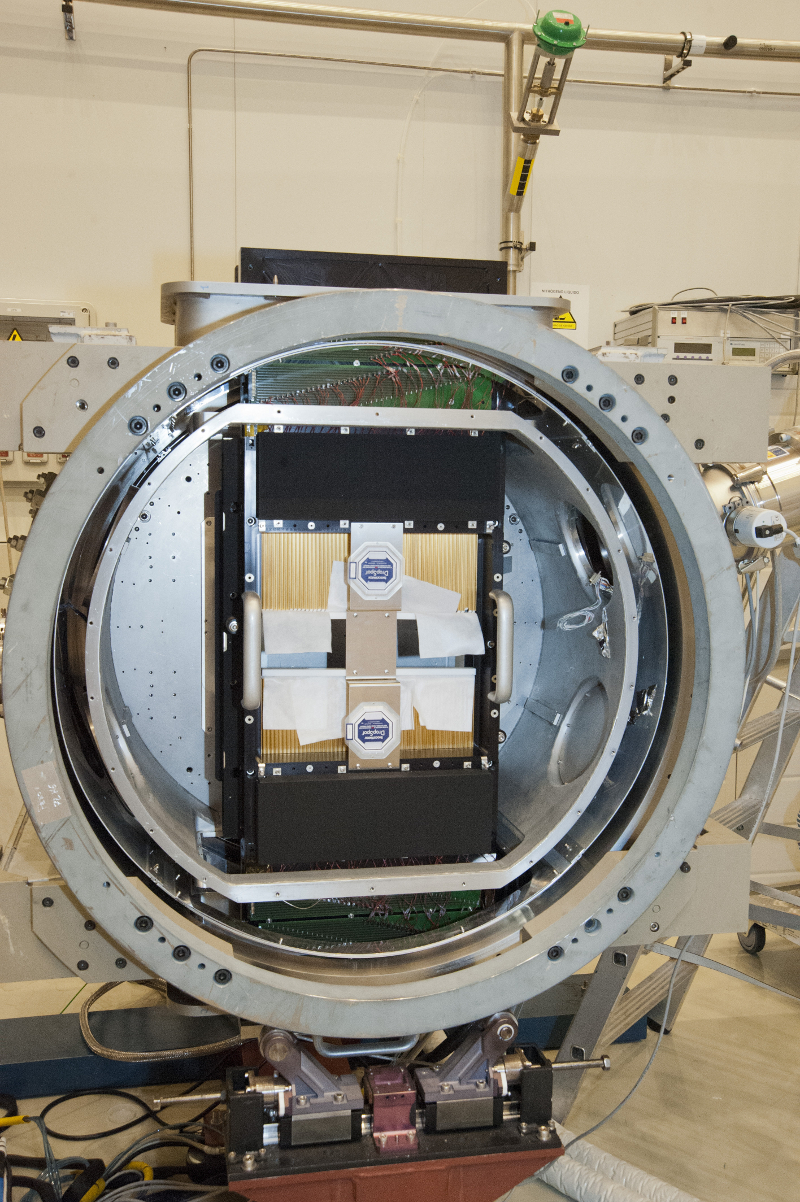
\includegraphics[height=0.5\linewidth]{DSC_9546}}
\subfloat {
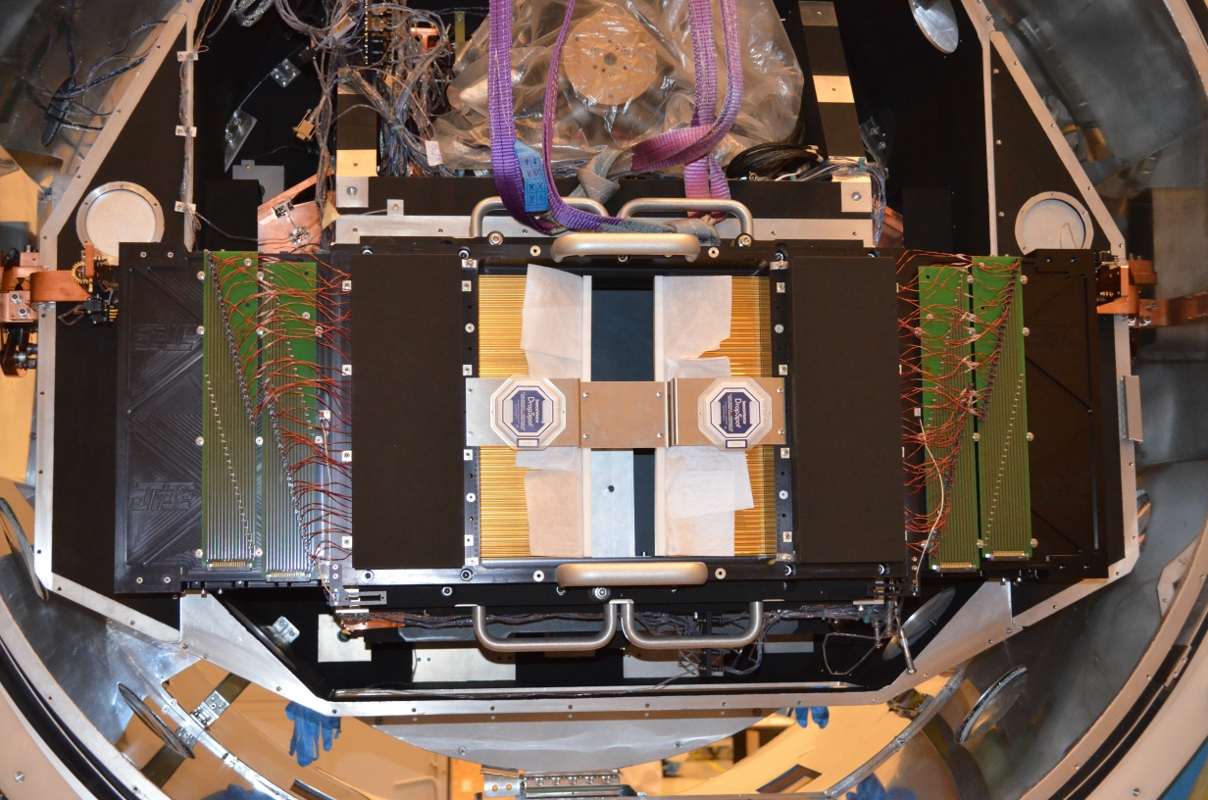
\includegraphics[width=0.7\linewidth]{DSC_0750}}
\caption{Unidad de rendijas configurables de EMIR}
\label{fig:CSUreal}
\end{figure}

EMIR rotará alrededor de su eje óptico durante el apuntado y operación, llevando
consigo a la CSU.  A efectos prácticos, esto significa que la CSU puede
configurarse en cada posición de apuntado del telescopio con ángulo de posición
en el rango [0,180] según las necesidades del usuario, como se muestra en la Figura
\ref{fig:CSU1}. Al ser simétrica, abarca todo el rango de giro posible, y puede 
estar colocada en cualquier punto del espacio visible (área de cielo observable
de dimensiones mucho mayores que las del subsistema). Llamamos ``apuntado'' a
una posición concreta de la CSU, especificada por un centro $(x,y)$ y un ángulo
de rotación, junto con la configuración de cada una de las 55 barras.

\begin{figure}[!htb]
\centering
\subfloat[CSU] {

\includegraphics[height=0.5\linewidth]{CSU}
\label{fig:CSU0}}
\subfloat[Rotación de la CSU] {
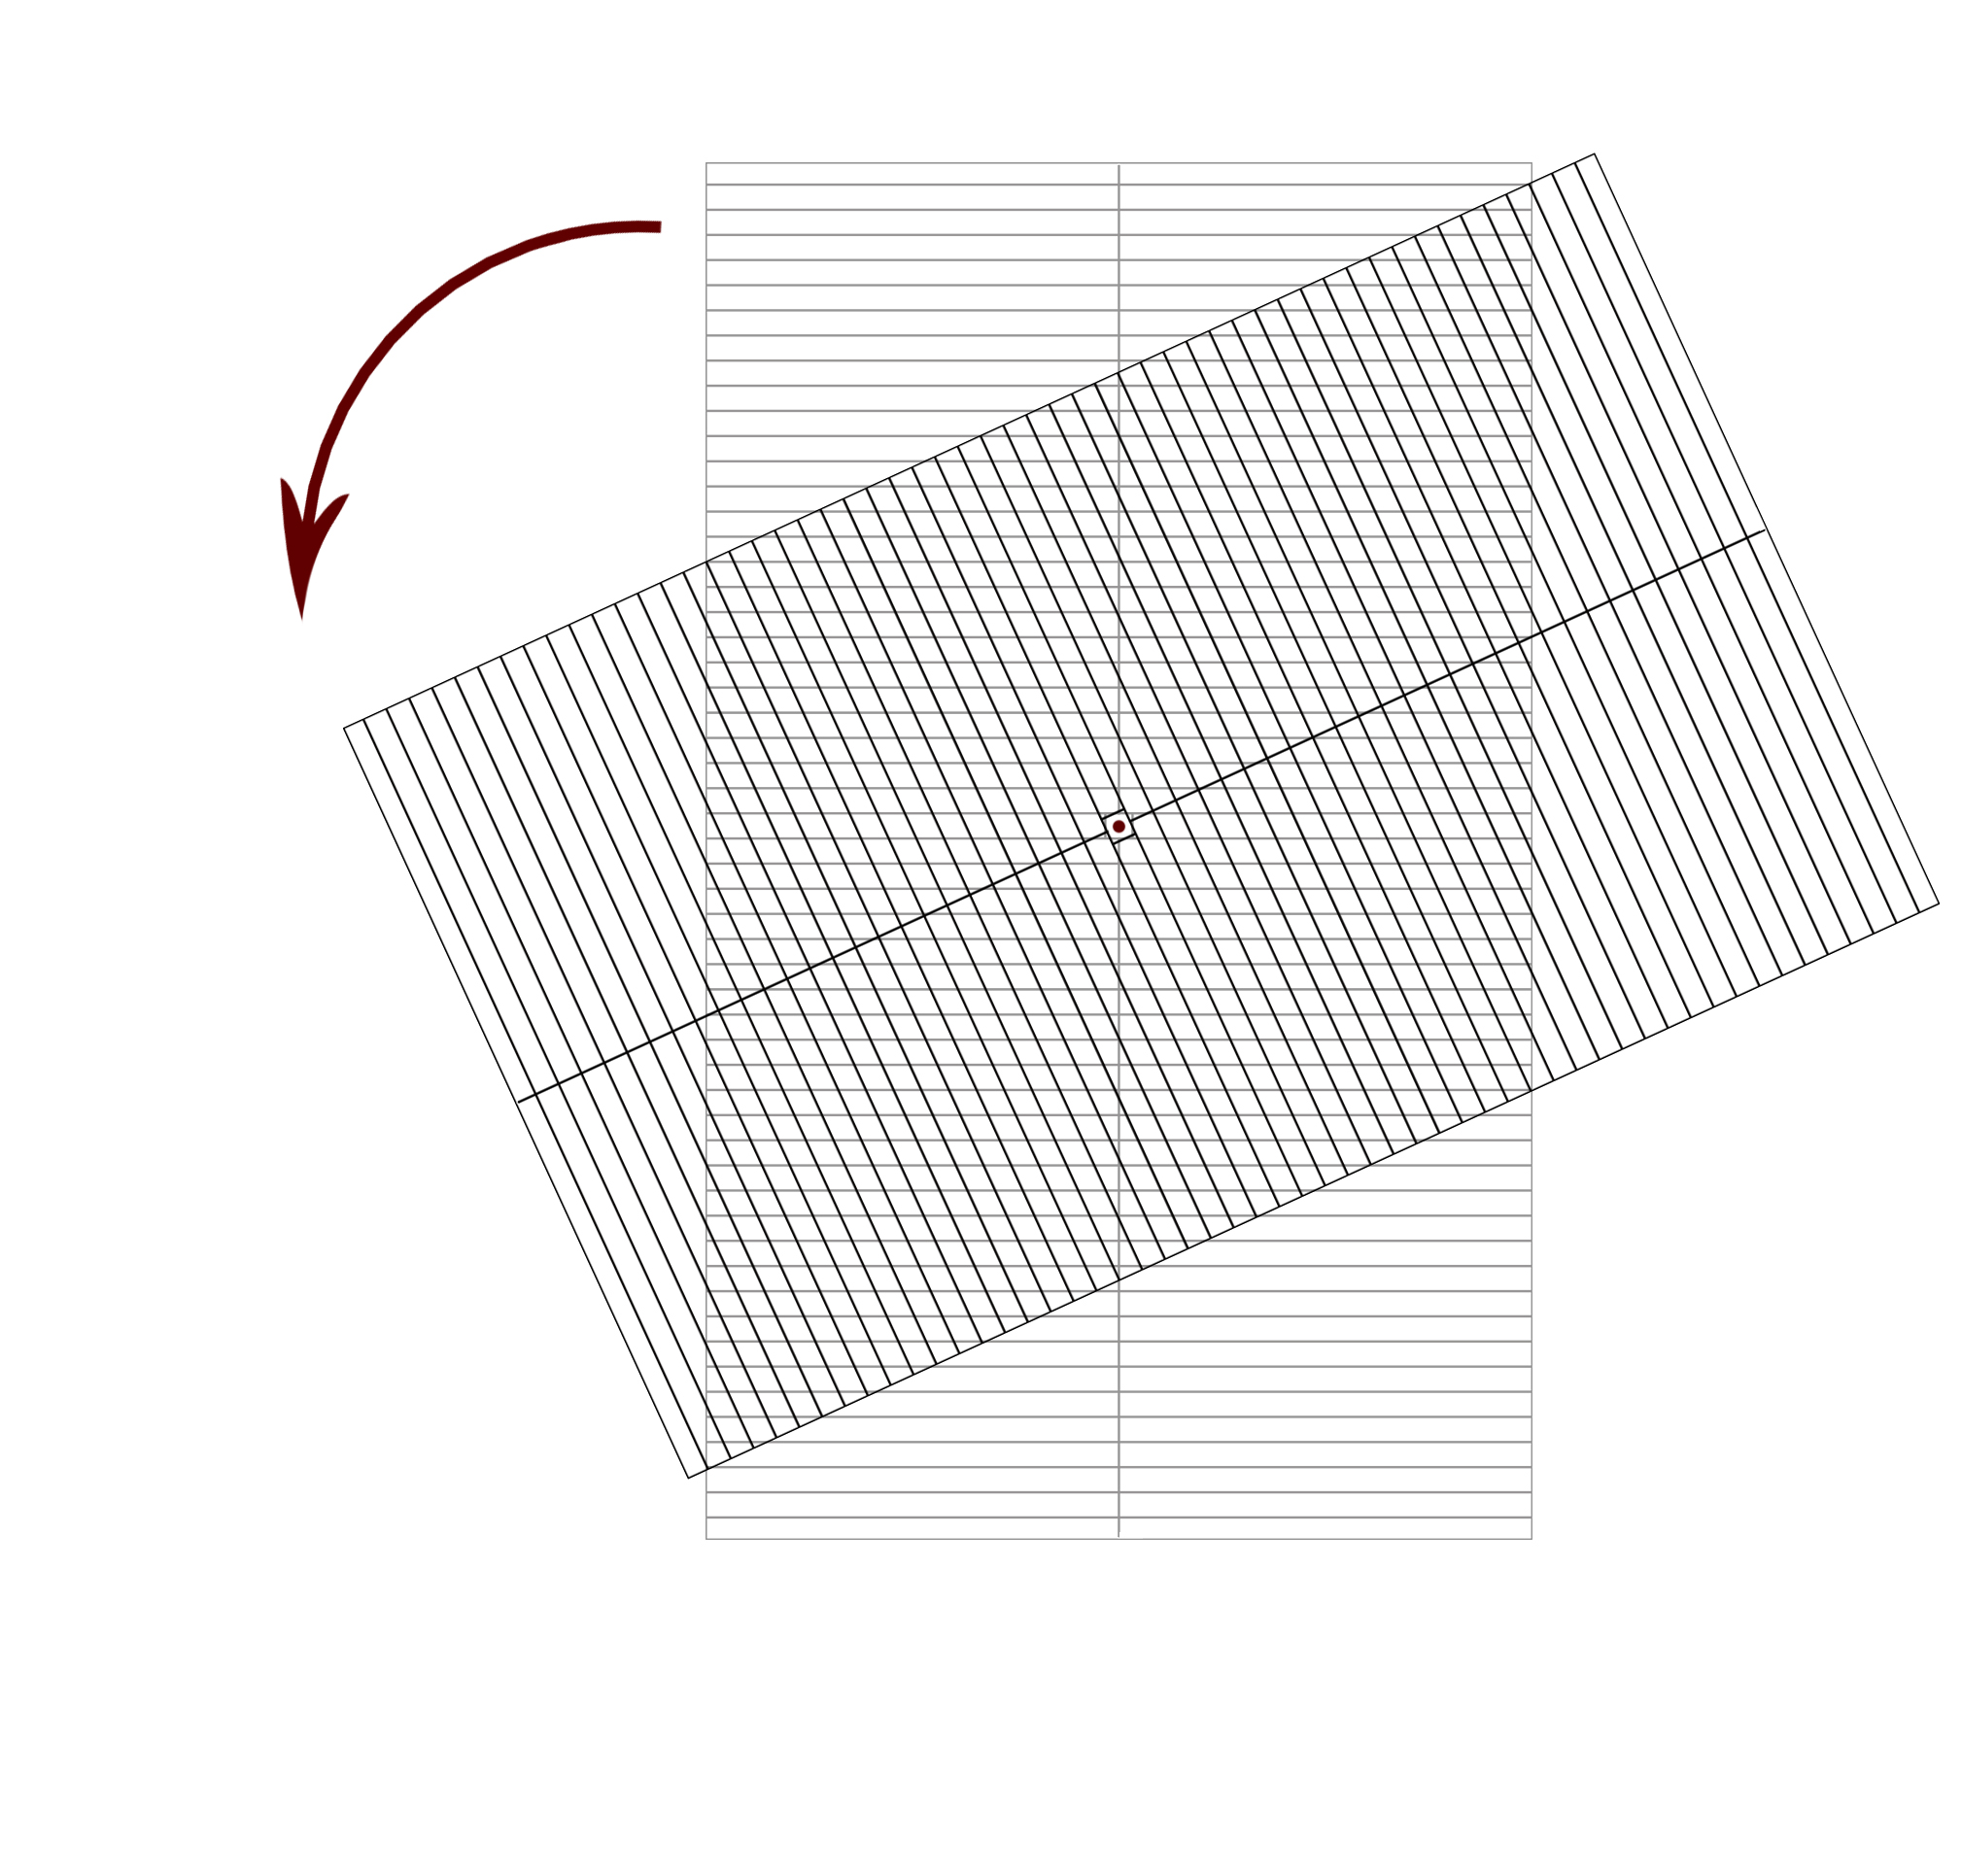
\includegraphics[width=0.5\linewidth]{CSU-giro}
\label{fig:CSU1}}
\caption{Representación gráfica de una CSU}
\end{figure}

Generalmente, para observar todos los objetos de interés astronómico de un
determinado campo es necesario utilizar más de un apuntado. Debido a que el
proceso de observación (medida) en cada apuntado de la CSU es muy lento, se hace
necesario minimizar el número de apuntados para cubrir todos, o al menos la
mayoría de  objetos de alta prioridad.  Para solucionar este problema se ha
desarrollado en el marco de este PFC una aplicación escrita en C++ que, dada una
entrada de puntos a medir, devuelve una lista de apuntados que resuelven el
problema. La Figura \ref{fig:CSU2} muestra un ejemplo de apuntado para cuatro
objetos.

\begin{figure}[!htb]
\centering
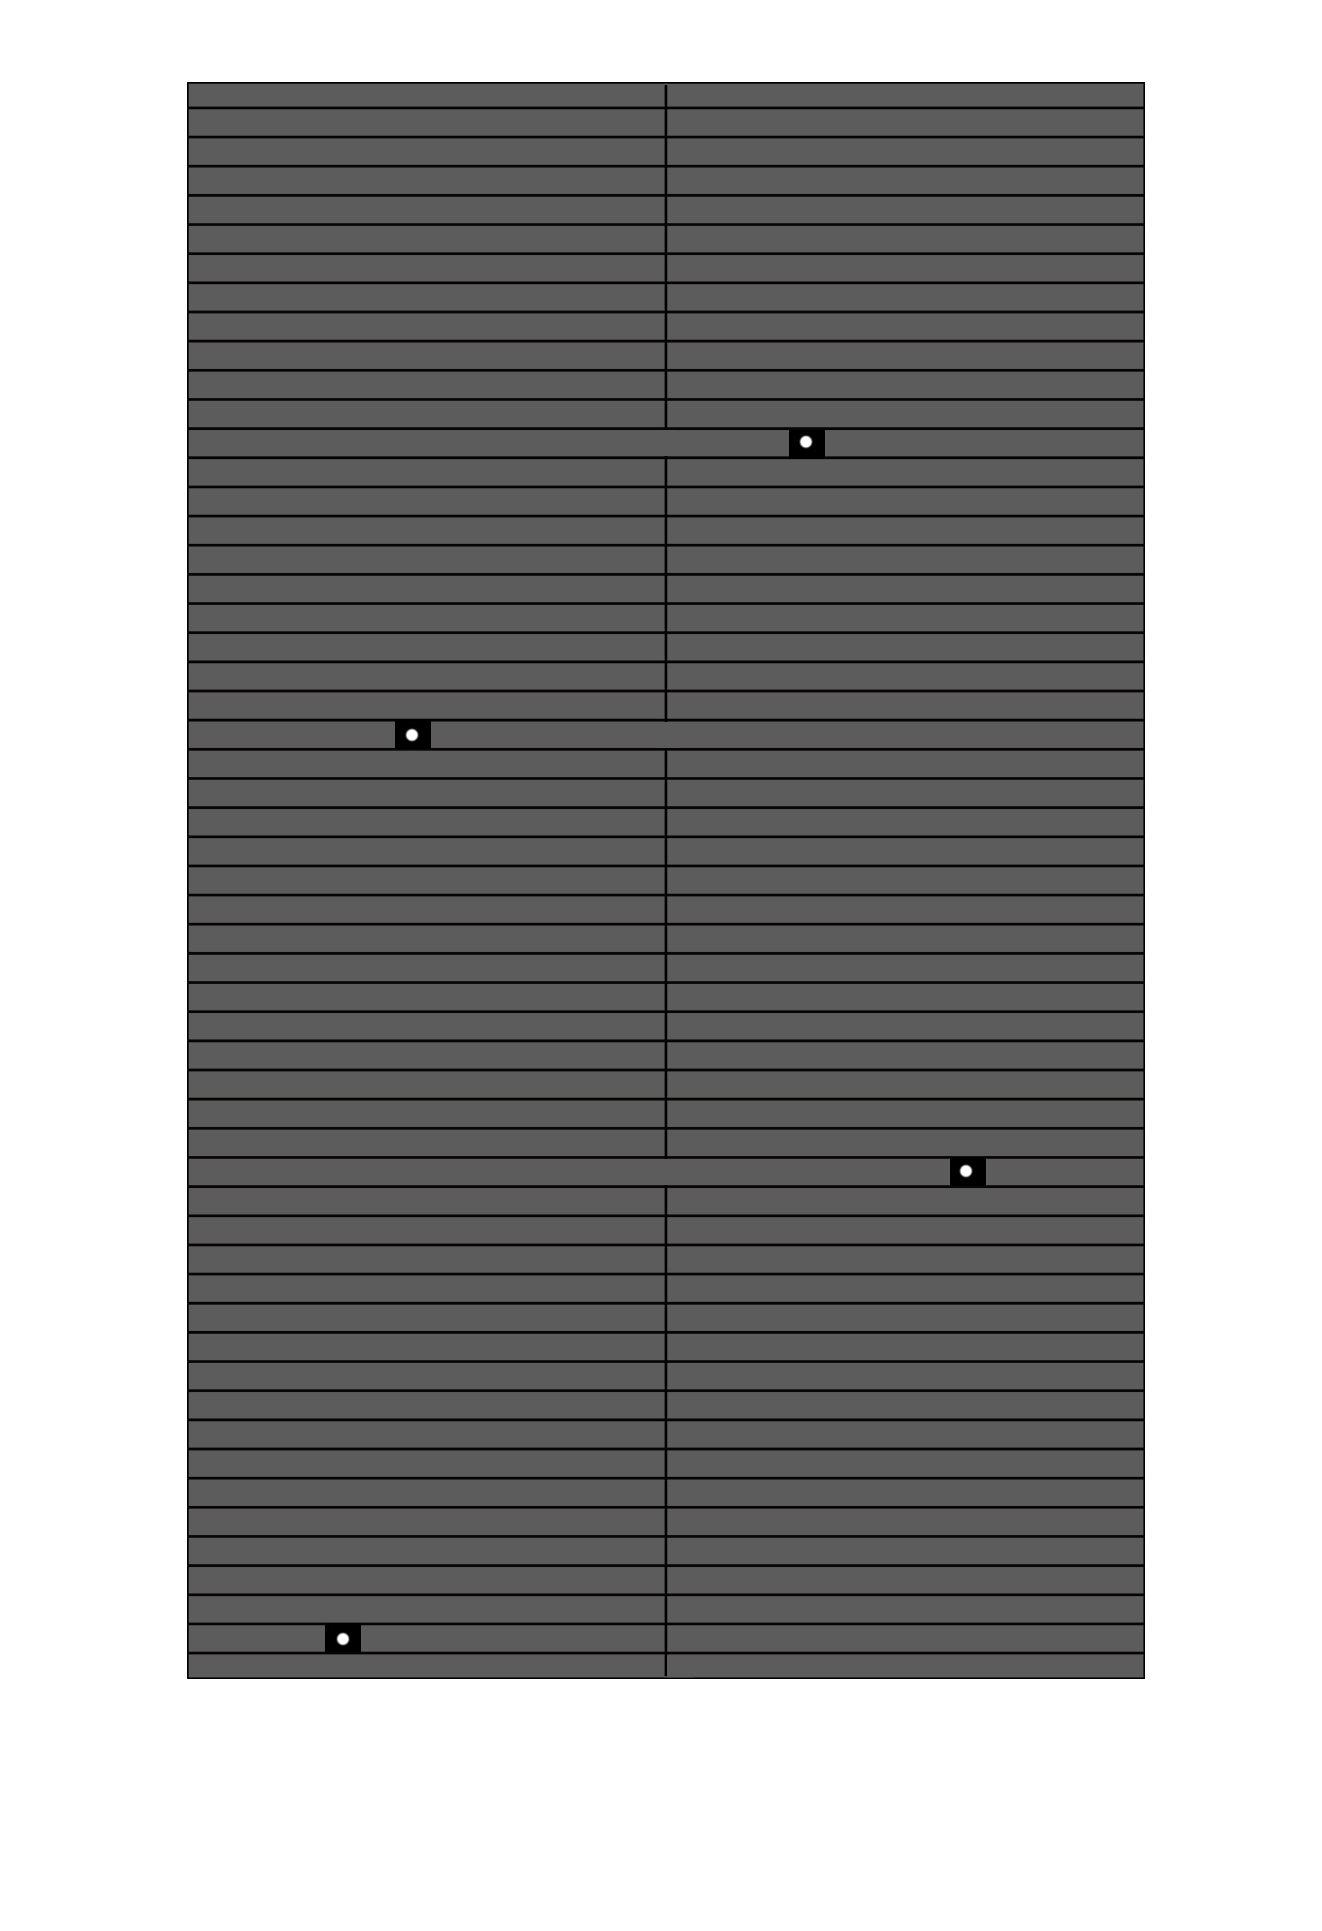
\includegraphics[height=0.5\linewidth]{CSU-puntos}
\caption{Apuntado con 4 barras ocupadas}
\label{fig:CSU2}
\end{figure}

\subsection{Beam Switching}

El \textit{beam switching} es un método para obtener mediciones de un objeto de
una forma más precisa. El método consiste (aplicado a nuestro problema) en medir
tanto la luz perteneciente al objeto celeste como la de la propia bóveda
celeste, mover a continuación ligeramente la posición del medidor (dejando los
objetos donde antes no había nada) y volver a realizar las mediciones oportunas.
La Figura \ref{fig:beams} muestra un ejemplo explicativo. De esta forma se
obtienen una serie de valores que pueden ser procesados posteriormente por el
investigador.

\begin{figure}[!htb]
\centering
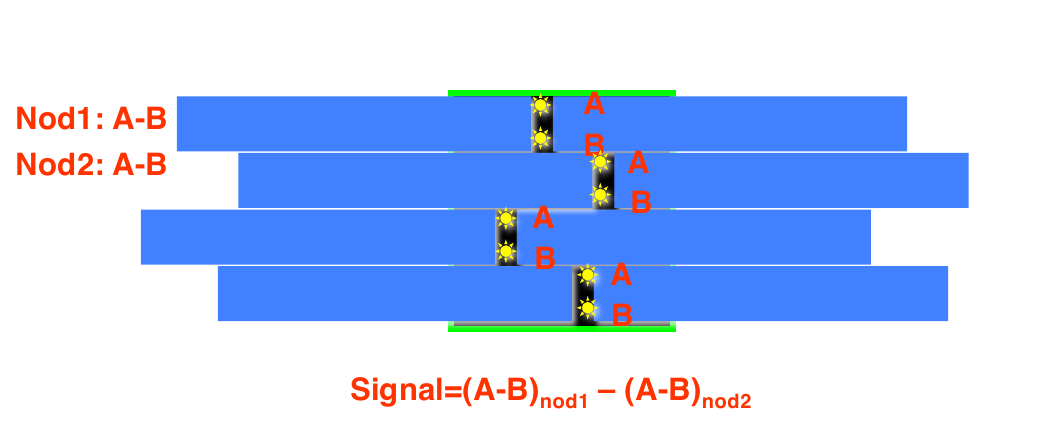
\includegraphics[width=0.7\linewidth]{beamexplication}
\caption{Muestra de funcionamiento de \texttt{beam switching}}
\label{fig:beams}
\end{figure}

 
%
% ---------------------------------------------------
%
% Proyecto Final de Carrera: EMIR
% Autor: Pedro Hernández Martín <alu3679@etsii.ull.es>
% Capítulo: Estado del arte
% Fichero: Cap2_estado_del_arte.tex
%
% ----------------------------------------------------
%

\chapter{Objetivos} \label{chap:objetivos}

A continuación se listan los objetivos propuestos para este PFC,
de los cuales se han completado totalmente la mayoría mientras que
la dedicación a algunos de ellos se ha tenido que minimizar u obviar por falta de tiempo.

\begin{itemize}
\item Desarrollar una aplicación plenamente funcional que resuelva de modo
óptimo el problema de optimización de apuntados de la CSU del proyecto EMIR.
\item Realizar la resolución del problema en el menor tiempo posible.
\item Tratar las prioridades entre elementos observables.
\item Contemplar el uso por parte de los investigadores del método conocido como \textit{beam switching}.
\item Estudiar diferentes alternativas para la resolución del problema
computacional planteado, así como realizar una revisión bibliográfica de métodos
y técnicas de optimización relacionados con dicho problema.
\item Involucrarse en el conocimiento de un proyecto real de investigación
aplicada, el proyecto EMIR, siendo capaz de aportar al mismo un elemento
importante para su desarrollo.
\item Conocer con cierto grado de detalle la tecnología involucrada en el
desarrollo del proyecto EMIR así como el contexto en el que esta información se
utiliza.
\item Participación en un proceso de ``release'' de software (empaquetado,
testing, validación, etc).
\item Poner en práctica de modo efectivo en una aplicación real los
conocimientos adquiridos en la titulación en materia de Programación e
Ingeniería del Software.
\item Diseño e implementación de una interfaz gráfica amigable al usuario. Éste
punto ha sido eliminado por falta de tiempo, dejando como parte gráfica la
visualización de los resultados.
\end{itemize}
 
%
% ---------------------------------------------------
%
% Proyecto Final de Carrera: EMIR
% Autor: Pedro Hernández Martín <alu3679@etsii.ull.es>
% Capítulo: Estado del arte
% Fichero: Cap2_estado_del_arte.tex
%
% ----------------------------------------------------
%

\chapter{Tecnologías y herramientas relacionadas} \label{chap:estado}

A continuación se dan a conocer algunas tecnologías o conocimientos que han 
resultado necesarios para el proyecto, o se han planteado como tal.

\section{Parsers XML}

Un analizador sintáctico \cite{Wiki:2013:ANA} (en inglés parser) es una de las 
partes de un compilador que transforma su entrada en un árbol de derivación.
El análisis sintáctico convierte el texto de entrada en otras estructuras 
(comúnmente árboles), que son más útiles para el posterior análisis y capturan 
la jerarquía implícita de la entrada. Un analizador léxico crea tokens de una 
secuencia de caracteres de entrada y son estos tokens los que son procesados 
por el analizador sintáctico para construir la estructura de datos, por ejemplo 
un árbol de análisis o árboles de sintaxis abstracta.

El uso más común de los analizadores sintácticos es como parte de la fase de 
análisis de los compiladores, de modo que tienen que analizar el código fuente 
del lenguaje. Los lenguajes de programación tienden a basarse en gramáticas 
libres de contexto, debido a que se pueden escribir analizadores rápidos y 
eficientes para éstas.

Las gramáticas libres de contexto tienen una expresividad limitada y sólo pueden 
expresar un conjunto limitado de lenguajes. Informalmente la razón de esto es
que la memoria de un lenguaje de este tipo es limitada, la gramática no puede 
recordar la presencia de una construcción en una entrada arbitrariamente larga y
esto es necesario en un lenguaje en el que, por ejemplo, una variable debe ser
declarada antes de que pueda ser referenciada. Las gramáticas más complejas no 
pueden ser analizadas de forma eficiente. Por estas razones es común crear un 
analizador permisivo para una gramática libre de contexto que acepta un
superconjunto del lenguaje (acepta algunas construcciones inválidas); después
del análisis inicial las construcciones incorrectas pueden ser filtradas.

Puesto que la entrada y salida de la aplicación \CSUO{} se encuentran
descritas en XML, se aprovechará unos de los muchos parsers opensource
disponibles en Internet para, por un lado, comprobar que la entrada no tiene
errores, y por otro, transformar estos datos en las estructuras que necesita
nuestra aplicación. Existen muchas librerías que nos facilitan la lectura y
escritura de este tipo de ficheros; como se desea distribuir la aplicación para
que cualquiera la pueda utilizar, es muy recomendable emplear una librería
estándar (o muy popular) que sea eficiente.

\subsection{Xerces-C++}

Xerces-C++ \cite{Web:Xerces} es un analizador de XML válido escrito en un
subconjunto portable de C++. Xerces-C++ hace que sea fácil darle a su aplicación
la capacidad de leer y escribir datos XML. Proporciona una biblioteca compartida
para analizar, generar, manipular y validar documentos XML utilizando DOM, SAX y
APIs de SAX2. Xerces-C++ es fiel a la recomendada XML 1.0 y a muchos estándares
asociados.

El analizador proporciona un alto rendimiento, modularidad y escalabilidad.
Código fuente, muestras y documentación de la API se proporcionan con el
analizador. Para que resulte portable se ha tenido cuidado de hacer un uso
mínimo de las plantillas, no usa RTTI, y un uso mínimo de \texttt{\#ifdefs}. Sin
embargo este analizador se descartó debido a que encontramos otro que se
ajustaba mejor a nuestras necesidades.

\subsection{Mini-XML}

Mini-XML \cite{Web:Mini-XML} es una pequeña librería XML que se utiliza
para leer y escribir XML y archivos de datos estilo XML en nuestra aplicación
sin necesidad de usar grandes librerías no estandarizadas. Mini-XML sólo
requiere de un compilador de C compatible con ANSI (GCC funciona, al igual que 
la mayoría de compiladores ANSI C).

Mini-XML permite la lectura de UTF-8 y UTF-16 y la escritura de UTF-8 en
ficheros XML codificados y cadenas. Los datos se almacenan en una lista enlazada
con estructura de árbol, conservando la jerarquía de datos XML, y los nombres de 
elementos arbitrarios, atributos y valores de atributos son soportados sin
límites preestablecidos, pero sólo disponibles en memoria.

Este parser no estaba disponible para su descarga por problemas de servidores en
el momento que se buscó, por lo que fue descartado.

\subsection{TinyXML}

TinyXML \cite{Web:TinyXML} es un analizador de XML para C++ simple, pequeño,
mínimo, que se puede integrar fácilmente en otros programas. Lee XML y crea
objetos de C++ que representan el documento XML. Los objetos se pueden
manipular, modificar y guardar de nuevo como XML.

TinyXML es de tipo DOM, cuya una curva de aprendizaje es muy elevada y, además,
suele ser lento en comparación con los SAX, por lo que también se ha descartado.

\subsection{PugiXML}

Pugixml \cite{Web:pugixml} es una librería ligera de procesamiento de XML para
C++. Consiste en una interfaz tipo DOM con ricas capacidades de
recorrido/modificación, un analizador XML extremadamente rápido que construye el
árbol DOM desde un archivo/buffer XML, y una implementación XPath 1.0 para las
consultas de los árboles por datos complejos. También está disponible el soporte
completo para Unicode, con variantes de interfaz Unicode y conversiones entre
diferentes codificaciones Unicode. La biblioteca es muy fácil de transportar y
fácil de integrar y utilizar. Pugixml es desarrollado y mantenido desde 2006 y
tiene muchos usuarios. Todo el código se distribuye bajo la licencia MIT, por lo
que es totalmente gratuito para su uso en las aplicaciones de código abierto y
propietario.

Pugixml permite un procesamiento muy rápido, práctico y eficiente de documentos
XML. Sin embargo, desde que pugixml tiene un analizador DOM, no puede procesar
documentos XML que no caben en la memoria; y el analizador no valida, así que se
descarta porque no cumple con los propósitos de este PFC.

\subsection{RapidXML}

RapidXml \cite{Web:rapidxml} es un intento de crear el analizador XML más rápido
posible, sin perder capacidad de uso, portabilidad y compatibilidad razonable
W3C. Es un analizador in situ escrito en C++ moderno, con velocidad de análisis
próxima a la de la función strlen, ejecutada en los mismos datos.

RapidXml ha estado presente desde 2006, y está siendo utilizado por muchas
personas. HTC lo utiliza en algunos de sus teléfonos móviles. No se ha elegido
este analizador por los mismos motivos que se descartó el TiniXML.

\subsection{Libxml++} \label{sec:LIBXML}

libxml++ \cite{Cumming:2012:LIB} es un wrapper de C++ para la librería libxml
XML parser.

Libxml2 es el analizador XML de C y es un kit de herramientas desarrolladas para
el proyecto Gnome (pero utilizable fuera de la plataforma Gnome), que es
software libre disponible bajo la licencia MIT. XML es un metalenguaje para
diseñar lenguajes de etiquetas. HTML es el lenguaje de etiquetas más conocido. 
Aunque la librería está escrita en C, es posible encontrar adaptaciones en muchos
lenguajes en otros entornos. 

Libxml2 es conocido por ser muy portable, la librería debe generarse y trabajar
sin graves problemas en una variedad de sistemas (Linux, Unix, Windows, CygWin,
MacOS, MacOS X, RISC Os, OS/2, VMS, QNX, MVS, VxWorks, ...).

Libxml2 implementa varios estándares existentes relacionadas con lenguajes de
etiquetas:
the XML standard, Namespaces in XML, XML Base, RFC 2396: Uniform Resource 
Identifiers, XML Path Language (XPath) 1.0, HTML4 parser, XML Pointer Language 
(XPointer) Version 1.0, XML Inclusions (XInclude) Version 1.0, ISO-8859-x 
encodings, así como rfc2044 [UTF-8] y rfc2781 [UTF-16] Unicode encodings (y más
si se utiliza de apoyo iconv), XML Catalogs Working Draft 06 August 2001, 
Canonical XML Version 1.0, Relax NG, ISO/IEC 19757-2:2003, W3C XML Schemas Part
2: Datatypes REC 02 May 2001, W3C xml:id Working Draft 7 April 2004.

Debido a su portabilidad, número de estándares acogidos y gran contenido y
soporte disponible en la red, sobre todo por el hecho de estar presente en Gnome
(y ser éste uno de los entornos de escritorio más extendidos en distribuciones
de Linux), ha sido el candidato elegido para apoyar nuestra aplicación.
Se explica de qué manera se integra en \CSUO{} en el capítulo referente a
la aplicación \ref{chap:aplication}.

\section{Allegro} \label{sec:Allegro}

Para visualizar gráficamente los resultados de nuestra aplicación, se emplea
Allegro \cite{Hargreaves:2010:ALL}. Allegro es una librería libre y de código
abierto para la programación de videojuegos desarrollada en lenguaje C. Allegro
es un acrónimo recursivo de «Allegro Low Level Game Routines» (rutinas de bajo
nivel para videojuegos). Fue originalmente creado por Shawn Hargreaves para el
Atari ST a principios de 1990, pero la idea fue abandonada más adelante.
Alrededor de 1998, Allegro se ramificó en varias versiones. Se creó una
distribución para Microsoft Windows (WinAllegro) y también una para Unix
(XwinAllegro). Allegro 4.0 sería la primera versión estable de Allegro para
múltiples plataformas.

La librería cuenta con funciones para gráficos, manipulación de imágenes, texto,
sonidos, dispositivos de entrada (teclado, ratón y mandos de juego) y
temporizadores, así como rutinas para aritmética de punto fijo y acceso al
sistema de archivos. Hay 2 versiones de Allegro que cuentan con soporte oficial
por parte de los desarrolladores, la versión clásica (Allegro 4) y la nueva
versión (Allegro 5). La versión más reciente de Allegro 4 incluye soporte para
el manejo de archivos de datos y una implementación por software de funciones
para gráficos en 3D. La versión 5 de Allegro cuenta con una nueva API y cambia
la implementación por software de las rutinas gráficas por una implementación
basada en OpenGL o Direct3D.

Aunque Allegro ofrece una API en lenguaje C, actualmente existen envolventes y 
librerías adicionales que permiten utilizarlo en otros lenguajes como Python, D, 
Lua y Pascal.

La versión 4 de Allegro, versión utilizada en nuestra aplicación,
cuenta con varias librerías adicionales creadas por la comunidad de usuarios;
entre ellas se encuentran las que agregan soporte para varios formatos de
archivo multimedia (por ejemplo PNG, GIF, JPEG, MPEG, Ogg, MP3 y más).

Librerías adicionales como AllegroGL y OpenLayer utilizan OpenGL para añadir 
aceleración por hardware a los programas de Allegro. Tenga en cuenta que, en 
combinación con Glide y MesaFX (utilizando el hardware 3dfx), AllegroGL es una
de las pocas soluciones de código abierto disponibles para hardware de 
aceleración 3D bajo DOS.

%%%%%%%%%%%%%%%%%%% Fig. %%%%%%%%%%%%%%%%%%%%%%%%%%%%%%%%%%%
\begin{figure}[!htb]
\centering
\subfloat[Ejemplo 3D]{
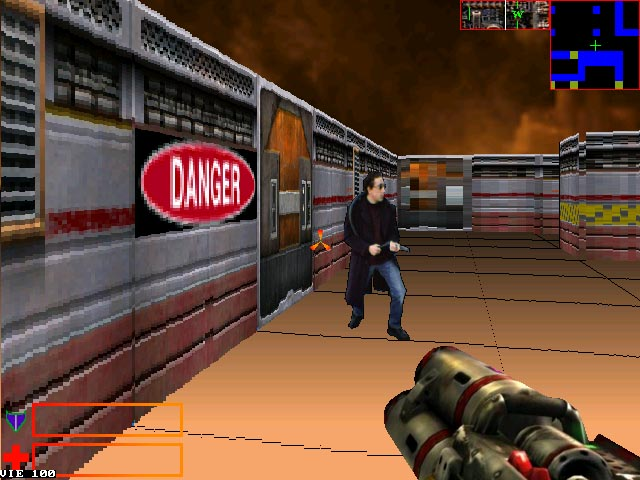
\includegraphics[height=5cm]{Allegroexample1}
\label{fig:allegro3d}}
\subfloat[Ejemplo 2D]{
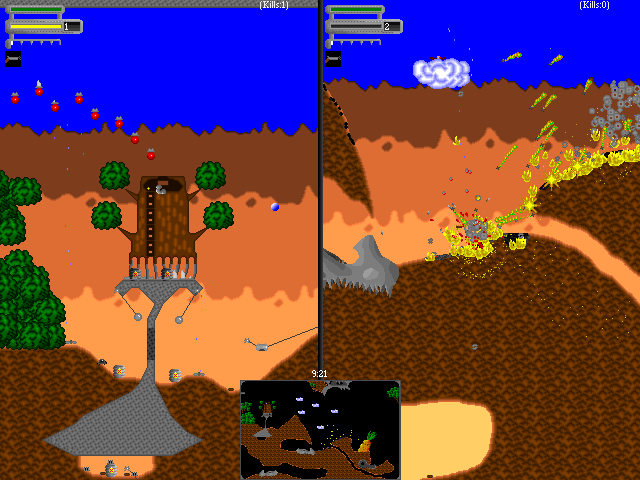
\includegraphics[height=5cm]{Allegroexample2}
\label{fig:allegro2d}}
\caption{Ejemplos de la potencia gráfica de la librería Allegro}
\end{figure}
%%%%%%%%%%%%%%%%%%%%%%%%%%%%%%%%%%%%%%%%%%%%%%%%%%%%%%%%%%%%%%

\section{Algoritmos de clustering}
El primer enfoque de nuestra aplicación fue basarnos en la densidad de objetos
en el espacio, con el objetivo de centrarnos en áreas con mayor densidad (y por 
tanto, mayor número de objetos a introducir en la CSU). Dado que nos interesa 
agrupar elementos en un espacio reducido, delimitado por el tamaño de la CSU,
prestaremos atención a los algoritmos de clustering.

Un algoritmo de agrupamiento (en inglés, clustering) es un procedimiento de 
agrupación de una serie de vectores de acuerdo con un criterio. Esos criterios
son por lo general distancia o similitud. La cercanía se define en términos de
una determinada función de distancia, como la euclídea, aunque existen otras más
robustas o que permiten extenderla a variables discretas. La medida más
utilizada para medir la similitud entre los casos es las matriz de correlación 
entre los n$\times$n casos. Sin embargo, también existen muchos algoritmos que
se basan en la maximización de una propiedad estadística llamada verosimilitud.

Generalmente, los vectores de un mismo grupo (o clústers) comparten propiedades
comunes. El conocimiento de los grupos puede permitir una descripción sintética
de un conjunto de datos multidimensional complejo. De ahí su uso en minería de 
datos. Esta descripción sintética se consigue sustituyendo la descripción de 
todos los elementos de un grupo por la de un representante característico del 
mismo.

Ninguno de los algoritmos clásicos de clustering cumple con las características
exactas de nuestro problema, por lo que se tuvo que investigar un poco como
funciona cada uno de ellos. Hay una gran diversidad de algoritmos, algunos muy
antiguos y otros bastante recientes, pero casi todos tienen en común la
dependencia de cierto tipo de parámetros condicionantes. Este tipo de
dependencia varía bastante el resultado, y no siempre resulta fácil saber qué se
está cambiando o cómo adecuarlo a nuestro problema. A continuación se muestran
algunos de los que se han analizado y estudiado con el fin de utilizarlos.

\subsection{K-means}

K-means \cite{Hartigan:1979:KMC} es un método de agrupamiento, que tiene como
objetivo la partición de un conjunto n en k grupos en el que cada observación
pertenece al grupo más cercano a la media. Esto da lugar a una 
compartimentación del espacio de datos en celdas de Voronoi.

El problema es computacionalmente difícil (NP-duro). Sin embargo, hay
heurísticas eficientes que se emplean comúnmente y convergen rápidamente a un
óptimo local. Estos suelen ser similares a los algoritmos de
esperanza-maximización de mezclas de distribuciones gausianas por medio de un
enfoque de refinamiento iterativo empleado por ambos algoritmos. Además, los dos
algoritmos usan los centros que los grupos utilizan para modelar los datos, sin
embargo k-means tiende a encontrar grupos de extensión espacial comparable,
mientras que el mecanismo esperanza-maximización permite que los grupos tengan
formas diferentes.

%%%%%%%%%%%%%%%%%%% Fig. %%%%%%%%%%%%%%%%%%%%%%%%%%%%%%%%%%%
\begin{figure}[!htb]
\centering
\subfloat[Entrada]{
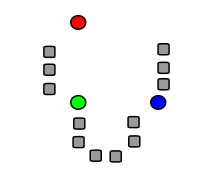
\includegraphics[height=2.5cm]{K_Means_Example_Step_1}
\label{fig:k_means1}}
\subfloat[Paso 1]{
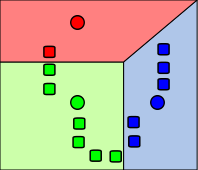
\includegraphics[height=2.5cm]{K_Means_Example_Step_2}
\label{fig:k_means2}}
\subfloat[Paso 2]{
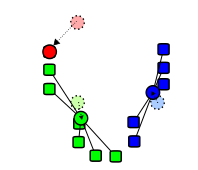
\includegraphics[height=2.5cm]{K_Means_Example_Step_3}
\label{fig:k_means3}}
\subfloat[Salida]{
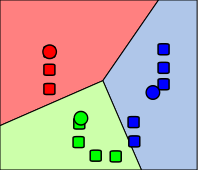
\includegraphics[height=2.5cm]{K_Means_Example_Step_4}
\label{fig:k_means4}}
\caption{Ejemplo de cómo funciona el K-means}
\end{figure}
%%%%%%%%%%%%%%%%%%%%%%%%%%%%%%%%%%%%%%%%%%%%%%%%%%%%%%%%%%%%%%

Como se trata de un algoritmo heurístico, no hay ninguna garantía de que
converja al óptimo global, y el resultado puede depender de los grupos
iniciales. Como el algoritmo suele ser muy rápido, es común para ejecutar
varias veces con diferentes condiciones de partida. Sin embargo, en el peor de
los casos, k-means puede ser muy lento para converger: en particular, se ha 
demostrado que existen conjuntos de determinados puntos, incluso en 2
dimensiones, en la que k-means toma tiempo exponencial.

\subsection{DBSCAN}

DBSCAN: Density-based spatial clustering of applications with noise (Agrupación
espacial basada en la densidad de aplicaciones con ruido) \cite{Ester:1996:SIC}, 
\cite{Wiki:2013:DBS} es un algoritmo de clustering de datos propuesto por Martin
Ester, Hans-Peter Kriegel, Jörg Sander y Xiaowei Xu en 1996. Se trata de un
algoritmo de clustering basado en la densidad, ya que encuentra un número de
clusters a partir de la distribución de la densidad estimada de nodos
correspondientes. DBSCAN es uno de los algoritmos de agrupamiento más común y
también el más citado en la literatura científica.

La definición de un conjunto en DBSCAN se basa en la noción de
accesibilidad-densidad. Básicamente, un punto $q$ es directamente accesible
desde un punto $p$ si no está más lejos que una distancia dada $\varepsilon$ (es 
decir, es parte de su $\varepsilon$-vecindad) y si $p$ está rodeado por
suficientes puntos de tal manera que uno pueda considerar $p$ y $q$ para ser
parte de un clúster. $q$ se denomina densidad alcanzable a partir de $p$ si hay
una secuencia de $p_1,\ldots,p_n$ de puntos con $p_1$ = p y $p_n$ = q donde cada 
$p_{i+1}$ es directamente accesible desde $p_i$.

Tenga en cuenta que la relación de la densidad alcanzable no es simétrica. $q$
podría estar al borde de un clúster, que tiene insuficiente cantidad de vecinos
a contar tan denso en sí. Esto detendría el proceso de encontrar una ruta que se 
detiene con el primer punto no denso. Por el contrario, empezar la ruta desde
$q$ podría encontrar un camino hasta $p$. Debido a esta asimetría, se introduce
la noción de densidad-conectada: dos puntos $p$ y $q$ están
densamente-conectados si hay un punto $o$ de tal manera que tanto $p$ como $q$
son la densidad alcanzable a partir de $o$. La densidad-conectada es simétrica.

Un clúster, que es un subconjunto de los puntos de la base de datos, satisface
dos propiedades:
\begin{itemize}
\item Todos los puntos dentro de la agrupación son mutuamente denso-conectados.
\item Si un punto está denso-conectado con cualquier punto de la agrupación, 
forma parte del grupo también.
\end{itemize}

DBSCAN requiere dos parámetros: $\varepsilon$ (EPS) y el número mínimo de puntos 
requeridos para formar un clúster (MinPts). Se inicia con un punto de partida 
arbitrario que no ha sido visitado. La $\varepsilon$-vecindad de este punto se 
recupera, y si contiene suficientes puntos, se inicia un clúster. De lo
contrario, el punto es considerado como ruido. Tenga en cuenta que este punto más 
adelante se podría encontrar en una $\varepsilon$-ambiente suficientemente
grande de un punto diferente y por lo tanto, formar parte de un clúster.

Si se encuentra un punto para ser una parte densa de un clúster, su 
$\varepsilon$-vecindad es también parte de ese grupo. Por lo tanto, se añaden
todos los puntos que se encuentran dentro de la $\varepsilon$-vecindad, así como
su propia $\varepsilon$-vecindad cuando también son densos. Este proceso
continúa hasta que el clúster  de densidad-conectada se halla por completo.
Entonces, un nuevo punto no visitado es recuperado y procesado, llevando al
descubrimiento de un clúster adicional o ruido.

%%%%%%%%%%%%%%%%%%%%% Fig. %%%%%%%%%%%%%%%%%%%%%%%%%%%%%%%%%%%
\begin{figure}[ht]
\centering
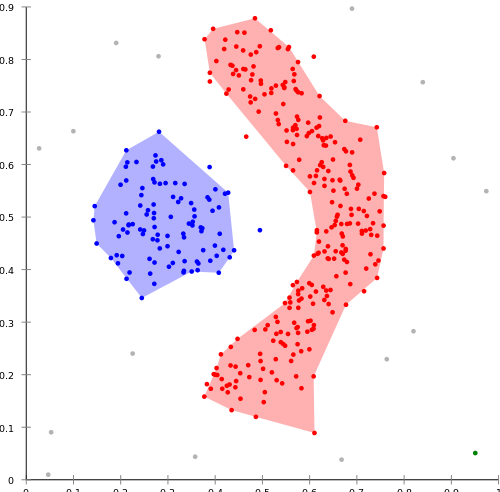
\includegraphics[height=10cm]{DBSCAN-density-data}
\label{fig:dbscan0}
\caption{Ejemplo del resultado del DBSCAN. Los puntos en gris son ruido}
\end{figure}
%%%%%%%%%%%%%%%%%%%%%%%%%%%%%%%%%%%%%%%%%%%%%%%%%%%%%%%%%%%%%

Ventajas
\begin{itemize}
\item DBSCAN no requiere especificar el número de grupos en los datos a priori,
como hace el k-means.
\item DBSCAN puede encontrar grupos de forma arbitraria. Se puede incluso
encontrar un clúster completamente rodeado por (pero no conectado a) un clúster
diferente. Debido al parámetro MinPts, el llamado efecto de enlace único
(diferentes grupos que se conectan por una delgada línea de puntos) se reduce.
\item DBSCAN tiene una noción de ruido.
\item DBSCAN requiere sólo dos parámetros y es insensible a la ordenación de los 
puntos en la base de datos. (Sin embargo, los puntos que se encuentren en el
borde de dos grupos diferentes pueden intercambiar pertenencia al clúster si se
cambia el orden de los puntos, y la asignación de clúster es único sólo hasta el
isomorfismo.)
\item DBSCAN está diseñado para su uso con bases de datos que pueden acelerar
las consultas de región, por ejemplo, mediante un árbol R*.
\end{itemize}

Desventajas
\begin{itemize}
\item La calidad de DBSCAN depende de la medida de distancia utilizado en la
función regionQuery(P,$\varepsilon$). La distancia métrica más común es la
distancia euclídea. Especialmente para los datos de grandes dimensiones, este 
indicador puede resultar casi inútil debido a la llamada ``maldición de la
dimensionalidad'', por lo que es difícil encontrar un valor adecuado para 
$\varepsilon$. Este efecto, sin embargo, también está presente en cualquier otro
algoritmo basado en la distancia euclídea. 
\item DBSCAN no puede agrupar conjuntos de datos correctamente si estos tienen
una gran diferencia en la densidad, ya que la combinación MinPts-$\varepsilon$
no puede entonces ser elegida adecuadamente para todos los grupos.
\end{itemize}

Todos estos algoritmos trabajan bastante bien cuando existen áreas más o menos 
diferenciadas unas de otras, sin embargo la mayoría de las ocasiones se trata
con datos dispersos de manera uniforme, con lo que el uso de estos algoritmos
puede ser más un inconveniente que una ventaja. Por otro lado, todos nuestros
objetos son relevantes, por lo que no podemos arriesgarnos a que se les tome por
ruido y, por lo tanto, se pierdan.

\section{Heurísticas}

En computación, dos objetivos fundamentales son encontrar algoritmos con buenos
tiempos de ejecución y buenas soluciones, usualmente las óptimas. Una heurística
es un algoritmo que abandona uno o ambos objetivos; por ejemplo, normalmente
encuentran buenas soluciones, aunque no hay pruebas de que la solución no pueda
ser arbitrariamente errónea en algunos casos; o se ejecuta razonablemente
rápido, aunque no existe tampoco prueba de que siempre será así. Las heurísticas
generalmente son usadas cuando no existe una solución óptima bajo las
restricciones dadas (tiempo, espacio, etc.), o cuando no existe del todo.

A menudo, pueden encontrarse instancias concretas del problema donde la
heurística producirá resultados muy malos o se ejecutará muy lentamente. Aun
así, estas instancias concretas pueden ser ignoradas porque no deberían ocurrir
nunca en la práctica por ser de origen teórico. Por tanto, el uso de heurísticas
es muy común en el mundo real.

A continuación se presenta la heurística que se ha evaluado, el método GRASP,
recomendada por el Doctor Marcos Moreno Vega.

\subsection{GRASP} \label{sec:grasp}

%http://catarina.udlap.mx/u_dl_a/tales/documentos/lii/hernandez_r_cm/capitulo3.pdf

La palabra GRASP proviene de las siglas de Greedy Randomized Adaptive Search
Procedures que se puede traducir como: Procedimientos de Búsqueda Voraces 
Aleatorizados y Adaptativos.

El método GRASP se introduce inicialmente por Feo y Resende en
\cite{Mladenovic:1997:VNS}. Es un procedimiento iterativo que consiste en: una
fase de construcción y una fase de búsqueda local. Se obtiene una solución
factible durante la fase de construcción aplicando un procedimiento voraz. 
En cada iteración del procedimiento voraz se agrega un nuevo elemento a la 
solución de acuerdo al valor de una función voraz. En lugar de escoger siempre
el mejor elemento candidato, se construye una lista con los mejores candidatos,
de donde se selecciona uno aleatoriamente. El término adaptativo se refiere al
hecho de que los beneficios asociados con cada elemento son actualizados en cada
iteración de la fase de construcción para reflejar los cambios producidos por 
selecciones previas. Una vez que se construye una solución utilizando un 
procedimiento voraz, se realiza un procedimiento de búsqueda local. 

En el Algoritmo \ref{algo:grasp1} se muestra el pseudocódigo de esta heurística
y en las Secciones \ref{subs:grasp1}, \ref{subs:grasp2} y \ref{subs:grasp3} se
explican los procedimientos que intervienen en el algoritmo.

\subsubsection{Algoritmo GRASP}
\begin{algorithm}[H]
\While {(criterio no satisfecho)} {

Construye una solución inicial usando el procedimiento voraz

Realiza una búsqueda local para mejorar la solución construida.

}
\caption{Pasos del \texttt{GRASP}}
\label{algo:grasp1}
\end{algorithm}

\subsubsection{Algoritmo de fase de construcción del GRASP.} \label{subs:grasp1}

Sea $f$ una función voraz, $\alpha$ es valor del parámetro para controlar la
aleatoriedad del procedimiento, $x$ una solución parcial, $C$ el conjunto de 
elementos candidato y $RCL$ la lista restringida de candidatos.

\begin{algorithm}[H]
$x \leftarrow {\O}$

Inicializa el conjunto de candidatos $C$

\While{$x$ infactible} {

  $a = min\{f(t), t \in C\}$

  $b = max\{f(t), t \in C\}$

  $RCL = \{c \in C, f(c)\le a + \alpha(b - a)\}$

  Seleccionar aleatoriamente un elemento $c \in RCL$

  $x \leftarrow x \cup\{c\}$

  Actualizar $C$
}

\caption{Pseudo-código constructivo para \texttt{GRASP}}
\label{algo:grasp2}
\end{algorithm}

\subsubsection{Algoritmo de búsqueda local.} \label{subs:grasp2}

Sea $f(x)$ la función a minimizar, $x$ una solución factible y $N(x)$ una
estructura de vecindad.

\begin{algorithm}[H]
$CriterioParada \leftarrow$ falso

\While{no se satisfaga $CriterioParada$} {

$x' = arg min\{f(y): y \in N(x)\}$

\eIf{$(f(x') < f(x))$} {$x \leftarrow x'$} {$CriterioParada \leftarrow$ cierto}
}
\caption{Pseudo-código de la búsqueda local}
\label{algo:grasp3}
\end{algorithm}
\subsubsection{Algoritmo voraz.} \label{subs:grasp3}

Sean $S$ una solución parcial, $E$ el conjunto factible de elementos que pueden 
ser añadidos a la solución parcial, $e_i·$ los elementos del conjunto $E$ y $g$
una función voraz. 

\begin{algorithm}[H]
$S \leftarrow \O$

  \While{$S$ no factible} {
  Evaluar la función voraz $g$ para cada elemento de E
  
	Seleccionar el mejor elemento $e \in E$ de acuerdo con el valor de la función voraz $g$
  
	$S \leftarrow S\cup\{e\}$
  
	Actualizar $E$
}
\caption{Método voraz para seleccionar los mejores elementos de la búsqueda}
\label{algo:grasp4}
\end{algorithm}

El objetivo de utilizar este método es mejorar la solución inicial obtenida con
nuestro algoritmo constructivo. Se explicará este proceso y hasta qué punto se ha
utilizado dentro de \CSUO{} en el Capítulo \ref{chap:aplication}.

%
% ---------------------------------------------------
%
% Proyecto Final de Carrera: EMIR
% Autor: Pedro Hernández Martín <alu3679@etsii.ull.es>
% Capítulo: Estado del arte
% Fichero: Cap2_estado_del_arte.tex
%
% ----------------------------------------------------
%

\chapter{Algoritmos} \label{chap:algorithm}

El objetivo del \CSUO{} es cubrir (abarcar) todos los objetos 
presentes en el campo observado, con el menor
número de apuntados posible. Para resolver este problema se plantearon varios
posibles frentes de actuación, explicados brevemente a continuación, y
exhaustivamente al final del Capítulo, donde se detalla el algoritmo
utilizado.

\section{Clustering} \label{sec:clustering}

El primer enfoque que se exploró fue el de utilizar la densidad que presentan los
objetos en su distribución espacial, de forma que se actúe primero sobre zonas donde existe un
mayor número de puntos. Para diferenciar las zonas en la que se agrupan los
objetos se ha utilizado el algorimo DBScan.
Para ello se partió del código \cite{Web:GITDBS} adaptándolo y traduciéndolo a C++.

El Algoritmo \ref{alg:pseudo-dbscan} muestra un pseudo-código para el DBScan.

\begin{algorithm}[H]
DBSCAN($D$, $eps$, $MinPts$) \{

   $C = 0$

   \For{(cada punto $P$ no visitado en el cjto de datos $D$)} {

      marcar $P$ como visitado

      $NeighborPts =$ regionQuery($P$, $eps$)

      \eIf{(sizeof($NeighborPts$) $< MinPts$)} { marcar $P$ como $RUIDO$ } {

         $C =$ siguiente cluster

         expandCluster($P$, $NeighborPts$, $C$, $eps$, $MinPts$)
      }
    }
\}

expandCluster($P$, $NeighborPts$, $C$, $eps$, $MinPts$) \{

  añadir $P$ al cluster $C$

  \For{(cada punto $P'$ en $NeighborPts$)} {% 

     \If{($P'$ no visited)} {%

       marcar $P'$ como visitado

       $NeighborPts' = $regionQuery($P'$, $eps$)

       \If{(sizeof($NeighborPts'$) $>= MinPts$)} {%

         $NeighborPts = NeighborPts$ unido a $NeighborPts'$
       }
     }

     \If{($P'$ todavía no es miembro de algún cluster)} {%

       añadir $P'$ al cluster $C$
     }
   }
\}

regionQuery($P$, $eps$) \{

   return todos los puntos vecinos de $P'$ (incluyendo $P$)
   %return all points within $P'$s eps-neighborhood (including $P$)
\}

\caption{Pseudo-código del algoritmo DBSCAN}
\label{alg:pseudo-dbscan}
\end{algorithm}

Los clusters obtenidos dependen de dos parámetros, \textit{eps} y \textit{Min\_Pts} que indican respectivamente la
distancia que se permite entre puntos y el número mínimo de objetos requeridos
para formar un cluster. 
Para obtener buenos resultados es necesario un
conocimiento profundo del problema de entrada, puesto que se deben variar los
parámetros según la distribución de los objetos del mismo. Este procesado
resulta costoso y poco rentable, puesto que por lo general este tipo de
algoritmos presenta pobres resultados en problemas con distribuciones espaciales
homogéneas.

%%%%%%%%%%%%%%%%%%% Fig. %%%%%%%%%%%%%%%%%%%%%%%%%%%%%%%%%%%
\begin{figure}[!htb]
\centering
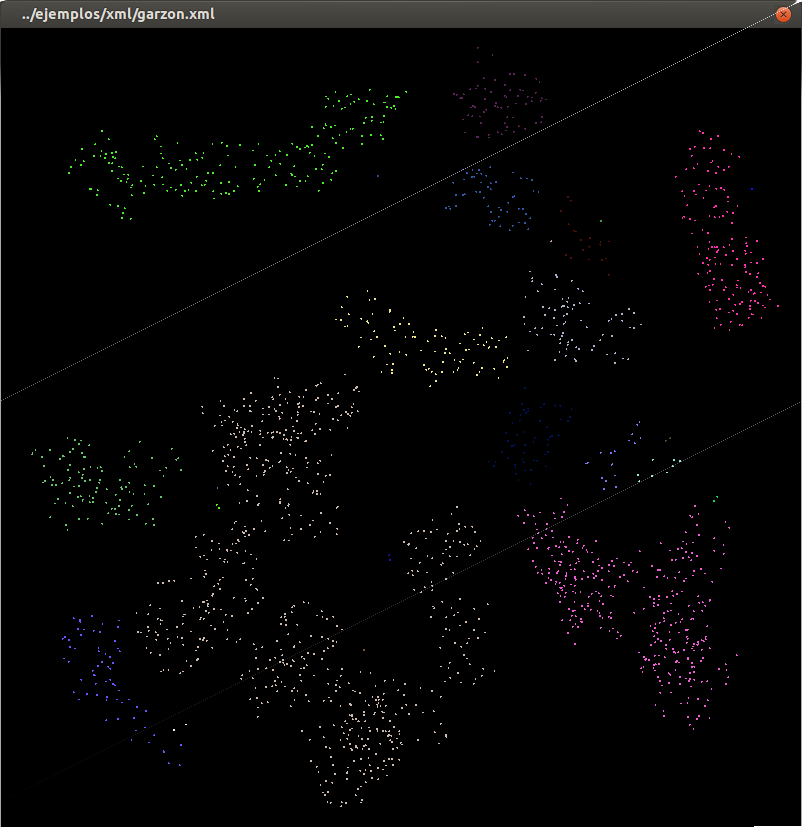
\includegraphics[width=0.7\linewidth]{dbscan-e86-m4}
\caption{Resultado de aplicar DBSCAN al \texttt{real1.xml}}
\label{fig:dbscan-e86-m4}
\end{figure}
%%%%%%%%%%%%%%%%%%%%%%%%%%%%%%%%%%%%%%%%%%%%%%%%%%%%%%%%%%%%%%

En la Figura \ref{fig:dbscan-e86-m4} se puede observar el resultado del
algoritmo aplicado al ejemplo \texttt{real1.xml} (cuya representación se puede
ver en la Figura \ref{fig:real1-in}). Los parámetros utilizados han sido 
\texttt{eps} = 86 y \texttt{MinPts} = 4.

Aunque se ha mantenido el uso del algoritmo DBScan como algo opcional
(utilizando la opción \texttt{--dbscan}) en el \CSUO{}, en virtud de los resultados obtenidos,
no se aconseja su uso por defecto.
Para algunas distribuciones de los objetos a observar, el uso previo del DBScan puede reducir algo
el tiempo de cómputo total, aunque esta reducción no es extensible a todas las instancias de entrada.
Si el usuario desea utilizar el DBScan, los parámetros a
modificar se encuentran en \texttt{bin/dbscan.C}, explicados en la Sección
\ref{sec:dbscan}.

\section{Grasp} \label{sec:grasp}

El algoritmo GRASP (\textit{Greedy Randomized Adaptive Search Procedure})
implementado no es exactamente el que se ha explicado en la Sección \ref{sec:grasp}, puesto que
empezó siendo una base para dicha heurística, pero no se llegó a desarrollar del
todo debido a los buenos resultados obtenidos por el algoritmo constructivo que
se explicará en la Sección \ref{sec:algconst}.  
Un posible pseudo-código del
algoritmo implementado es el que se muestra en el Algoritmo \ref{alg:grasp} y
consiste en generar varias soluciones aleatorias de las que se escoge la mejor
(aquella con menor número de apuntados). De esta mejor solución se separan
aquellos apuntados independientes (no colisionan con ningún otro, véase Sección
\ref{subsec:fase2}) de los que presentan algún solape con otra CSU. Los
independientes pasan a formar parte de la solución, pues han de estar
necesariamente para cubrir todos los objetos, mientras que los restantes se
introducen en un conjunto de CSUs candidatas (RCL), junto con el resto de
apuntados del resto de soluciones generadas. La RCL es ordenada de mejor a peor
resultado, y se va eligiendo una de las mejores candidatas aleatoriamente hasta
cubrir todos los puntos. 

\begin{algorithm}[H]
grasp($resultado$, $puntos$) \{

	Generar N posibles soluciones aleatorias
  
  $S_{ini} \leftarrow$ mejor solución generada

  $S_{fin} \leftarrow \O$

  \For{($\forall$ apuntado $C \in S_{ini}$)} {

    \If{($C$ no colisiona con $S_{ini}-\{C\}$)} {$S_{fin} += C$}
  }

  $RCL = S_{ini}\bigcup$ resto de soluciones generadas

	Ordenar $RCL$ por mejores apuntados

  \While{(puntos cubiertos en $S_{fin} < puntos$)} { %

  	$C = $ apuntado aleatorio $\in RCL$ elegido entre los mejores

    $C_{fin} += C$
  }

  \If {$C_{fin}$ mejor que $resultado$} {$resultado = C_{fin}$}

  return resultado

\}

\caption{Pseudo-código de un algoritmo GRASP}
\label{alg:grasp}
\end{algorithm}

\section{Algoritmo constructivo} \label{sec:algconst}

El algoritmo que construye la solución del problema se estructura en dos fases. 
En primer lugar se crea una solución inicial basada en la posición
cartesiana de los objetos en el espacio. Luego se hace un procesado de los
apuntados obtenidos, procurando eliminar aquellos que se puedan unificar para
dar lugar a un número menor de apuntados.

\subsection{Fase 1}
Los pasos que realiza este primer método que crea la solución inicial se
muestran en el Algoritmo \ref{alg:const1}.

\begin{algorithm}[H]
$Solucion$[tipo orden] $\leftarrow \O$

\For{(Cada tipo de ordenación)} {

  ordenar los objetos

  \While {(queden objetos por cubrir)} {

    	$p \leftarrow$ siguiente punto de la lista no eliminado

			$C =$ mejor CSU $\in$ crearApuntados($p$, $puntos$)

			$puntos -= \forall$ puntos $\in C$

			$Solucion$[tipo orden] $ = Solucion$[tipo orden] $ \bigcup\{C\}$
			
	}

}

$Sol =$ min($Solucion$[tipo orden])
\caption{Pseudo-código del algoritmo que crea la solución inicial}
\label{alg:const1}
\end{algorithm}

La función \texttt{crearApuntados()} se encarga de generar todas las posibles
CSUs válidas, y se entiende por válida cualquier CSU que tenga al menos un
objeto en alguna de sus barras, cuyo centro está situado sobre el objeto
especificado por parámetro. Una vez generado dicho apuntado, se realizan una
serie de movimientos de mejora sobre el mismo, con el fin de ``capturar'' todos
los objetos posibles. 
Los pasos se muestran en el Algoritmo \ref{alg:const2}. 

\begin{algorithm}[H]
$posibles \leftarrow \O$

\For{(Todas las rotaciones posibles)} {

    Crear $CSU$ con centro en $p$ 

    rellenar\_con\_puntos($CSU$, $puntos$)

    \While{(número de puntos en $CSU$ cambie)} {

        movimiento de mejora arriba

        rellenar\_con\_puntos($CSU$, $puntos$)

        movimiento de mejora abajo

        rellenar\_con\_puntos($CSU$, $puntos$)

        movimiento de mejora izquierda

        rellenar\_con\_puntos($CSU$, $puntos$)

        movimiento de mejora derecha

        rellenar\_con\_puntos($CSU$, $puntos$)

    }

    $posibles = posibles \bigcup\{CSU\}$

}
\caption{Pseudo-código del método de creación de apuntados}
\label{alg:const2}
\end{algorithm}

Los movimientos de mejora consisten en cambiar el centro del apuntado sin
modificar su ángulo de posición, con la restricción de que todos los objetos
que se encuentran en ese instante en sus barras, deben permanecer dentro de ese
apuntado. 
Cuando se dice que un punto está dentro de una CSU quiere decir que
dicha CSU tiene una barra en la que el objeto encaja perfectamente. 
Se permite que estos objetos ``inamovibles'' cambien de una barra a otra, se desplacen en una
misma barra, o se acerquen/alejen en menor o mayor medida del borde de la barra,
siempre y cuando sigan perteneciendo al apuntado. 
Este tipo de movimientos están explicados con mayor detalle en la Sección \ref{subsec:CSUmet}.

La Figura \ref{fig:mejora} muestra de forma gráfica estos pasos. En el primer
caso existe un apuntado con un objeto $A$ en su barra número 26. A continuación
se muestra el resultado del movimiento de mejora arriba, tras el que se ha
introducido el objeto $B$ en la barra 36, mientras que el objeto $A$ ha pasado a la barra 0. 
En el tercer paso se ha producido el movimiento de mejora abajo, que sitúa a $B$ en
la barra 54 y, por tanto, a $A$ en la barra número 18. 
El siguiente paso es realizar el movimiento de mejora izquierda. 
Dado que la coordenada X de $B$ es
menor que la de $A$, es $B$ el objeto que se sitúa más a la izquierda, permitiendo la
incorporación del objeto $C$ en la barra número 31. 
Por último se realiza el movimiento opuesto al anterior, el cual sitúa a $C$ en el borde derecho de la CSU.
El resultado global de estos movimientos ha sido pasar de un único objeto $A$ \textit{cubierto} por la
CSU considerada a \textit{cubrir} tres objetos.

%%%%%%%%%%%%%%%%%%%%% Fig. %%%%%%%%%%%%%%%%%%%%%%%%%%%%%%%%%%%
\begin{figure}[!htb]
\centering
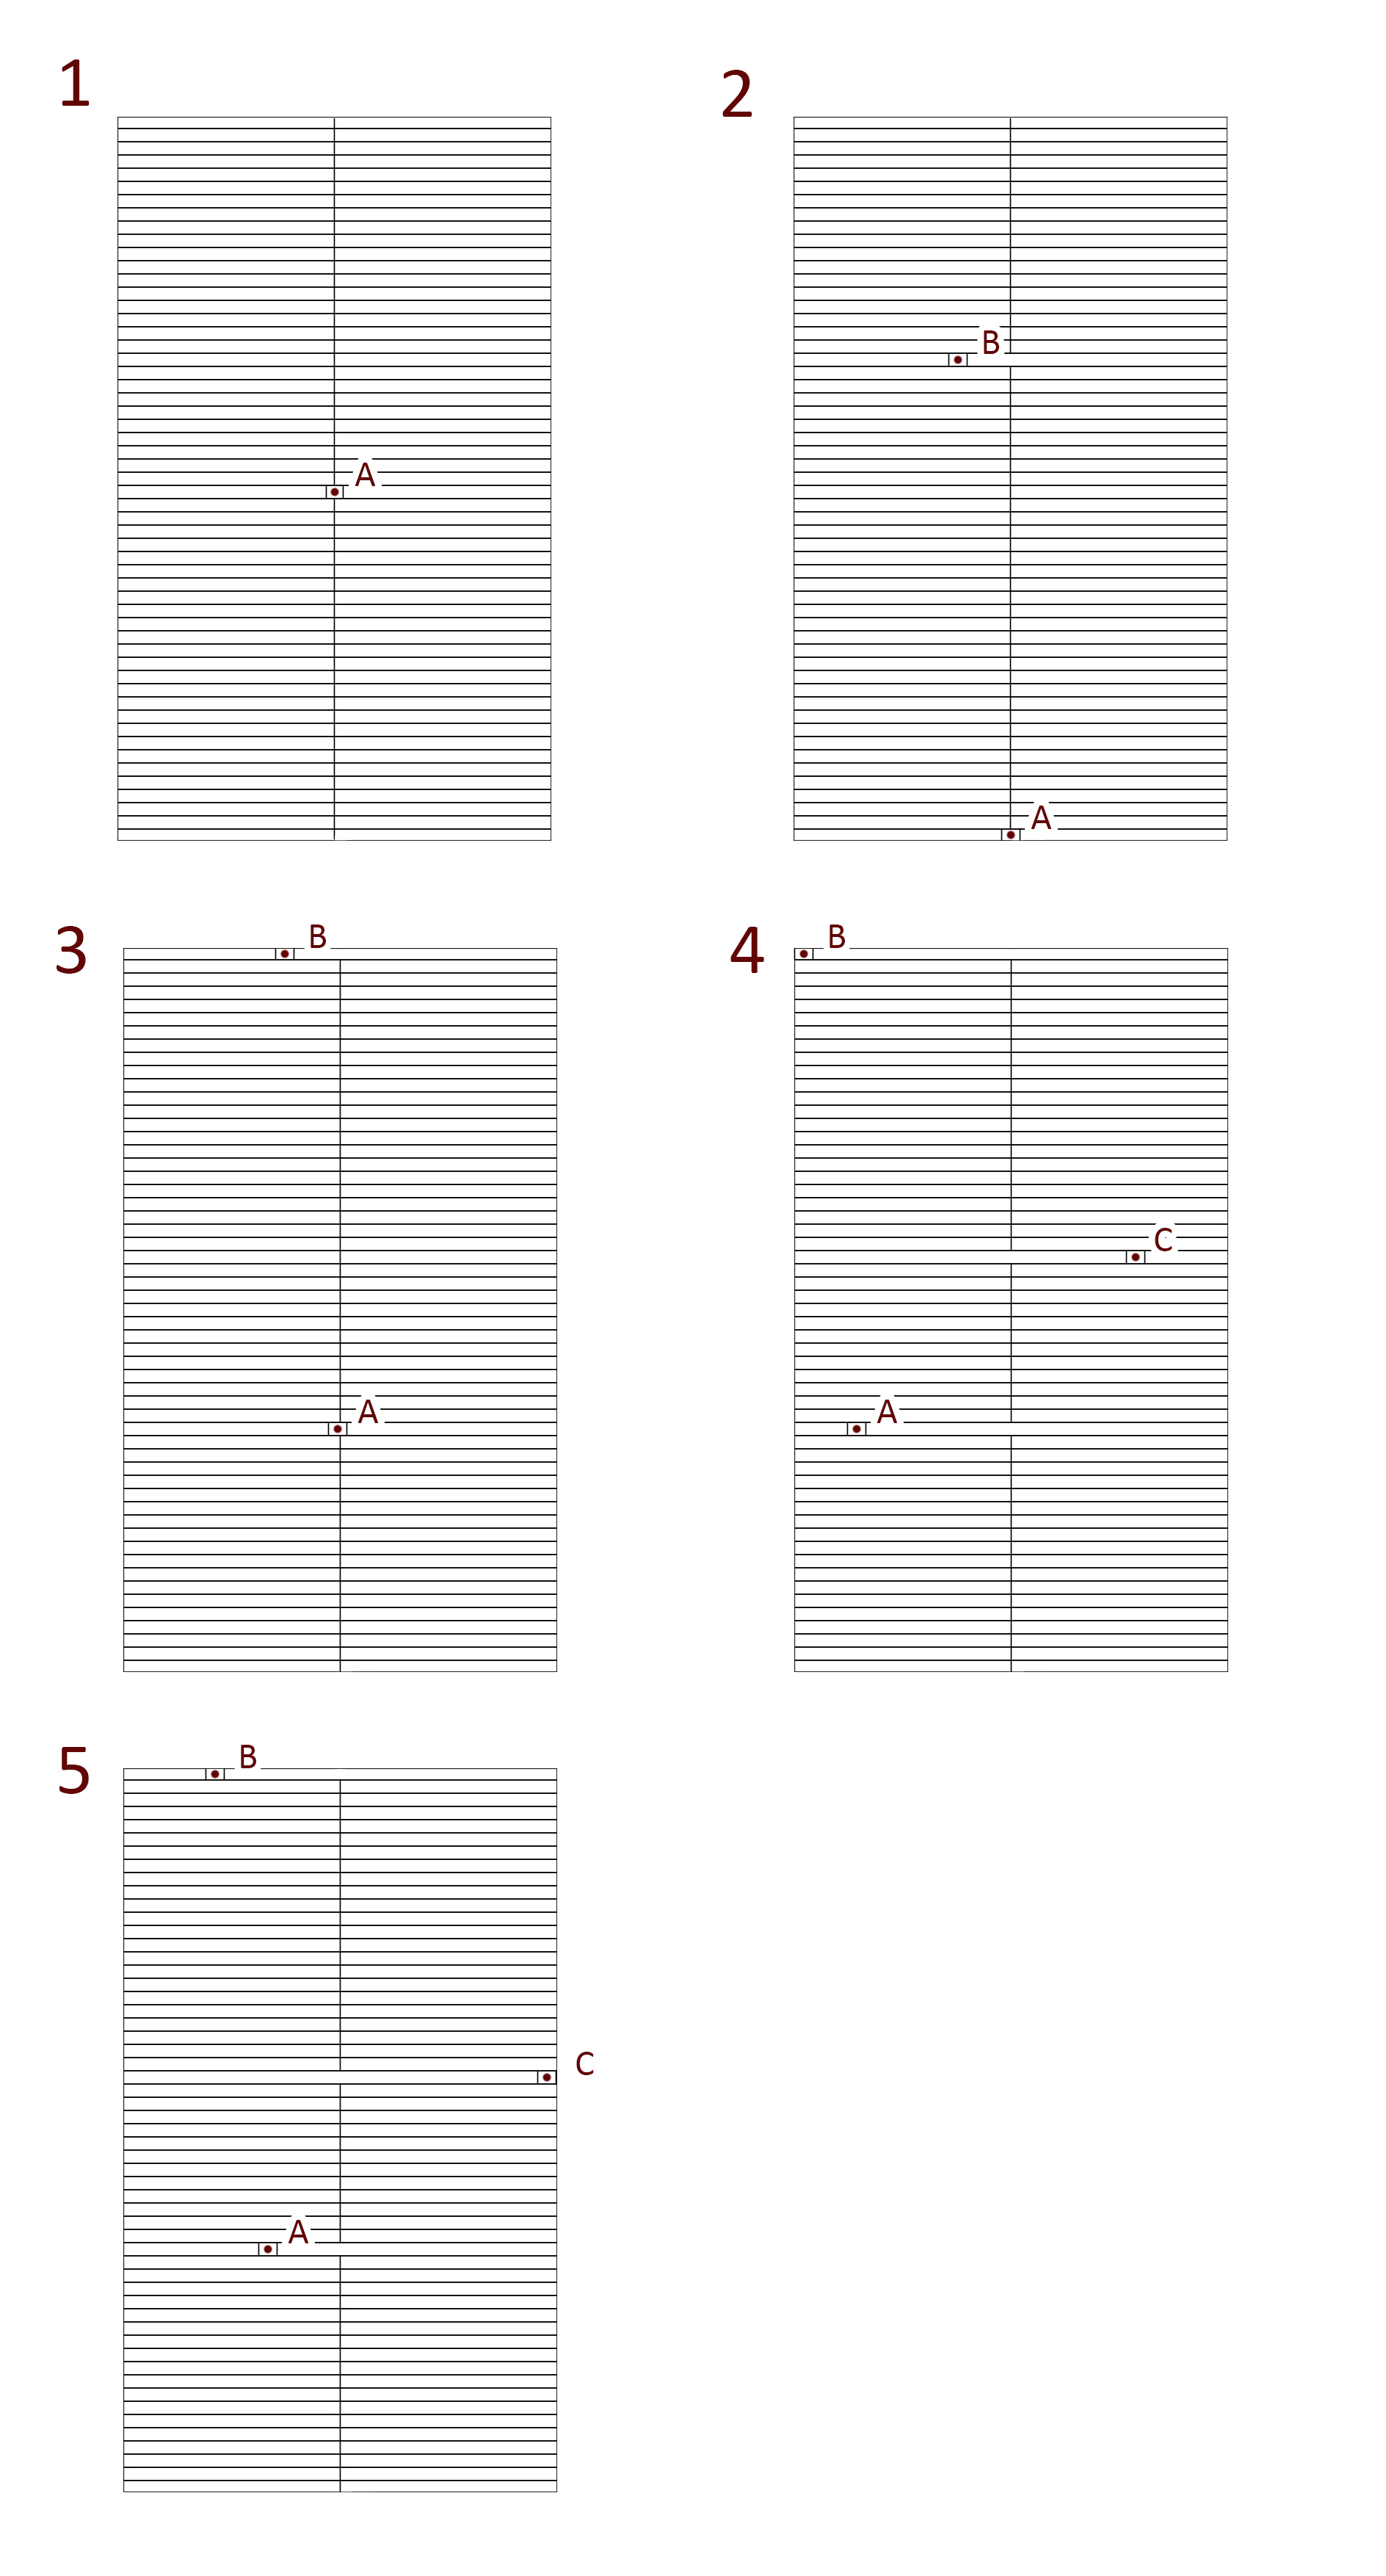
\includegraphics[width=0.7\linewidth]{CSU-algoritmo}
\caption{Movimientos de una CSU en el proceso de mejora}
\label{fig:mejora}
\end{figure}
%%%%%%%%%%%%%%%%%%%%%%%%%%%%%%%%%%%%%%%%%%%%%%%%%%%%%%%%%%%%%

La función \texttt{rellenar\_con\_puntos} del Algoritmo \ref{alg:const2} es la
que se encarga de analizar objeto por objeto si éste está dentro o no de un
apuntado, y en caso afirmativo, lo añade al mismo. 
Se considera que un punto está dentro de una CSU si:
\begin{itemize}
\item Se encuentra en el área abarcada por la CSU
\item Se sitúa sobre una barra que no tiene ningún objeto asociado a ella y 
\item El objeto cumple las restricciones físicas elegidas por el usuario, como puede ser que no
sobrepase el límite de distancia respecto al borde de la barra o que se
encuentre en la parte superior de la misma. 
\end{itemize}
Existen ocasiones en las que un
objeto no ajusta en una barra por un margen muy pequeño, bien porque la barra esté
ocupada ya por otro punto o porque esté en un rango no válido de la misma. 
En estas ocasiones, en lugar de descartar el objeto y buscar otro que sí ajuste, se ha hallado que
es preferible adaptar la CSU (siempre que ello sea posible, cumpliendo siempre con las
restricciones previamente definidas) para que éste entre en el apuntado.

\subsection{Fase 2} \label{subsec:fase2}
Una vez se tiene una solución al problema, es decir, un conjunto de apuntados
que ``cubren'' todos los objetos del problema, se intenta mejorar la solución eliminando o
reduciendo las colisiones entre apuntados. 
Diremos que un apuntado \textit{colisiona} con
otro cuando la intersección de las áreas cubiertas es no vacía.
Ello puede ocasionar que un objeto sea asociado a más de un apuntado.
Supongamos que se asocia con dos apuntados $A$ y $B$.
En este caso lo que
se intenta es crear un nuevo apuntado (CSU) $C$ con posición diferente a las
anteriores, que o bien las sustituya o bien consiga una mejora respecto a
alguna, es decir, $C$ mejor que $A$, $C$ mejor que $B$ o $C \equiv A \bigcup B$.
Esto se consigue iterando sobre el subconjunto de objetos son abarcados por $A$ y $B$
con un número mucho mayor de rotaciones de CSU. 
El Algoritmo \ref{alg:const3} presenta el esquema del algoritmo.

\begin{algorithm}[H]
$lista_{fin} \leftarrow \O$

$lista_{ini} =$ resultado

\While{(Mientras se mejore el resultado)} {

    $lista_{fin} =$ los que no colisionan con ninguno.

    \While{(queden objetos por cubrir)} {

        CSU $C \leftarrow$ primer apuntado $\in lista_{ini}$

        $subcto\_puntos = $ puntos de $C$

        Quitar $C$ de $lista_{ini}$

        \While{(queden CSUs $Q$ por mirar en $lista_{ini}$)} {

            \If{($Q$ colisiona con $C$)} {

                $subcto\_puntos += $ puntos de $Q$

                Quitar $Q$ de $lista_{ini}$

            }

        }

        \If{(colisión innecesaria)} {

            Obtener\_nuevos\_apuntados($subcto\_puntos$)

            \eIf{(consigue mejorar)} {$lista_{ini} +=$ nuevos apuntado } 
             {

                Introducir en $lista_{ini}$ los que se quitaron

                Poner en $lista_{fin}$ el apuntado $C$

             }

        }

    }

    $lista_{ini} = lista_{fin}$
}
\caption{Pseudo-código del algoritmo para reducir colisiones}
\label{alg:const3}
\end{algorithm}

Puesto que cada objeto puede tener una prioridad superior a la del resto (siendo
el 1 la mayor prioridad), se ha añadido también prioridad a los apuntados, de
modo que la prioridad del mismo la decide el objeto con mayor prioridad
contenido en dicha CSU. Una vez obtenidos los resultados, los apuntados son
ordenados por prioridades, situando primero los de mayor prioridad. 
En caso de que varios apuntados presenten la misma prioridad, se ordenarán según el número
de objetos que abarquen los mismos, colocando en primer lugar aquellos
apuntados cuyas barras estén completas.

En el Capítulo \ref{chap:aplication} se expone en detalle la implementación de todos
estos algoritmos y en qué punto del código de la aplicación se encuentran.


%
% ---------------------------------------------------
%
% Proyecto Final de Carrera: EMIR
% Autor: Pedro Hernández Martín <alu3679@etsii.ull.es>
% Capítulo: Estado del arte
% Fichero: Cap_aplicacion.tex
%
% ----------------------------------------------------
%

\chapter{La Aplicación \CSUO{}} \label{chap:aplication}
En este capítulo se explica en detalle la aplicación \CSUO{}, cómo
instalarla, cómo funciona, qué opciones tiene disponibles, etc. 
\CSUO{} ha sido desarrollada en C++ sobre una plataforma Linux, más
concretamente una distribución Ubuntu. 
En este Capítulo asumiremos que el usuario final dispone de un PC con esta distribución instalada y operativa.

La aplicación se entrega con la siguiente estructura de directorios:

\begin{itemize}
\item \texttt{bin}: Aplicación \CSUO{}.
\item \texttt{documentacion}: Documentación de código generada con Doxygen.
\item \texttt{ejemplos}: Algunos ejemplos de entrada.
  \begin{itemize}
  \item \texttt{conversor}: Aplicación para convertir archivos.
  \item \texttt{xml}: Ficheros XML correspondientes a los ejemplos.
  \end{itemize}
\item \texttt{map\_editor}: Aplicación para generar ejemplos sintéticos.
\item \texttt{memoriaEmir}: Código LaTEX de este documento.
\item \texttt{Resultados}: Ficheros de resultados de la aplicación.
\end{itemize}

Para la implementación de la aplicación se barajaron dos lenguajes de
programación, JAVA y C++, siendo elegido el segundo debido a la importancia
de una respuesta rápida a la hora de obtener soluciones por parte de la aplicación.
Se ha preferido utilizar un lenguaje compilado frente a uno interpretado en un intento
de satisfacer este requisito.
%%%%%%%%%%%%%%%%%%%%%%%%%%%%%%%
\section{Repositorio de código}
El código de la aplicación, así como el manual de la misma, se encuentra disponible en un
repositorio remoto alojado en Bitbucket \cite{Web:BIT} del que es posible descargarla.
Bitbucket es un servicio
de alojamiento basado en web, para proyectos que utilizan el sistema de
control de versiones Mercurial y/o Git. 
En el caso de este PFC hemos optado por utilizar Mercurial \cite{Web:MERCURIAL}.

%%%%%%%%%%%%%%%%%%%%%%%%%%%%%%%
\section{Instalación}
\subsection{Dependencias}
Antes de instalar la aplicación ha de asegurarse que se satisfacen todas las dependencias
de la misma, que se enumeran a continuación:
%%%%%%%%%%%%%%%%%%%%%%%%%%%%%%%
\subsubsection{make}
La herramienta make es necesaria para la automatización del compilado. Puede
instalarse desde la consola mediante:
\begin{lstlisting}[numbers=none]
sudo apt-get install make
\end{lstlisting}

%%%%%%%%%%%%%%%%%%%%%%%%%%%%%%%
\subsubsection{Compilador de C++}
El compilador \texttt{g++} es imprescindible para poder compilar el código.
Normalmente viene instalado por defecto en cualquier distribución Linux, pero si no fuera el caso, se puede
instalar usando:
\begin{lstlisting}[numbers=none]
sudo apt-get install g++
\end{lstlisting}
%%%%%%%%%%%%%%%%%%%%%%%%%%%%%%%
\subsubsection{libxml++}
Ésta librería es el parser XML que se ha usado con aplicación, tal y como se ha descrito en 
la Sección \ref{sec:LIBXML}. 
Para instalar \texttt{libxml++} se precisan los siguientes comandos:
\begin{lstlisting}[numbers=none]
sudo apt-get install libxml++2.6-dev libxml++2.6-doc
sudo apt-get install libgtkmm-2.4-dev
\end{lstlisting}
%%%%%%%%%%%%%%%%%%%%%%%%%%%%%%%
\subsubsection{Doxygen}
Doxygen \cite{Web:DOX} es un acrónimo de dox(document) gen(generator), generador de
documentación para código fuente.
Se trata de un generador de documentación para diversos lenguajes, entre ellos C++, C, o Java.
Dado que es fácilmente adaptable, funciona en la mayoría de
sistemas Unix así como en Windows y Mac OS X. 
La mayor parte del código de Doxygen ha sido escrito por Dimitri van Heesch.
Varios proyectos como KDE usan Doxygen para generar la documentación de su API.
KDevelop incluye soporte para Doxygen.

Para descargar Doxygen e intalarlo han de seguirse estos pasos:
\begin{itemize}
  \item Descargar y descomprimir el código fuente:
\end{itemize}
\begin{lstlisting}[numbers=none]
wget http://ftp.stack.nl/pub/users/dimitri/doxygen-1.8.4.src.tar.gz
tar -xzvf doxygen-1.8.4.src.tar.gz
\end{lstlisting}
\begin{itemize}
  \item Situarse en el directorio generado e intentar pre-instalar
    \begin{lstlisting}[numbers=none]
cd doxygen-1.8.4/
./configure
    \end{lstlisting}
  \item Si falla alguna de las comprobaciones, instalar dependencias.
    \begin{itemize}
      \item para graphviz:
        \begin{lstlisting}[numbers=none]
sudo apt-get install graphviz
        \end{lstlisting}
      \item para flex:
        \begin{lstlisting}[numbers=none]
sudo apt-get install flex
        \end{lstlisting}
      \item para bison:
        \begin{lstlisting}[numbers=none]
sudo apt-get install bison
        \end{lstlisting}
    \end{itemize}
  \item Una vez ejecutado el \texttt{./configure}
    \begin{lstlisting}[numbers=none]
make
sudo make install
    \end{lstlisting}
\end{itemize}

%%%%%%%%%%%%%%%%%%%%%%%%%%%%%%%
\subsubsection{LaTeX}
LaTeX \cite{Web:LATEX} es un sistema de composición de textos orientado
especialmente a la creación de libros, documentos científicos y técnicos.
LaTeX está formado por un gran conjunto de macros de TeX, escrito por Leslie
Lamport en 1984, con la intención de facilitar el uso del lenguaje de
composición tipográfica, TEX, creado por Donald Knuth. 
Es bien conocido en entornos académicos y científicos en los que 
la calidad tipográfica de los documentos generados es muy apreciada.
LaTeX es software libre bajo licencia LPPL.

Esta herramienta únicamente es necesaria si se necesita generar este documento, y
es posible instalarla con:
\begin{lstlisting}[numbers=none]
sudo apt-get install texlive-extra-utils
sudo apt-get install texlive-latex-extra
sudo apt-get install texlive-latex-recommended
sudo apt-get install texlive-full
sudo apt-get install texlive-science
\end{lstlisting}

%%%%%%%%%%%%%%%%%%%%%%%%%%%%%%%
\subsubsection{Allegro}
La librería Allegro, descrita en la Sección \ref{sec:Allegro}, se utiliza en el
\CSUO{} para la representación gráfica de los apuntados.

Para instalar Allegro se debe utilizar el siguiente paquete:
\begin{lstlisting}[numbers=none]
sudo apt-get install liballegro4.2-dev
\end{lstlisting}

Para utilizar Allegro en el código, basta con incluir el fichero de cabecera
\texttt{allegro.h} en el código tal como se muestra en la línea 1 del Listado \ref{codigo:allegro0}.
Este listado muestra cómo utilizar \texttt{Allegro} para inicializar y crear
una ventana.
\begin{lstlisting}[language=C++,basicstyle=\ttfamily\footnotesize,
                   caption={Ejemplo básico de uso de la librería Allegro},
                   label={codigo:allegro0}]
#include <allegro.h>
// Para poder cerrar la ventana pulsando el boton de cerrar
volatile int close_button_pressed = FALSE;
void close_button_handler(void) {
  close_button_pressed = TRUE;
}

int main (int argc, char **argv) {
  allegro_init(); // Inicializamos allegro
  install_keyboard();
  set_color_depth(16);
  set_window_title("Nombre de la ventana");
  // Definimos los tamanios de la ventana (800x800) pixeles de resolucion
  int w = 800, h = 800;
  //Generamos la ventana
  if(set_gfx_mode(GFX_AUTODETECT_WINDOWED,w,h,0,0) != 0) { //modo grafico
    set_gfx_mode(GFX_TEXT,0,0,0,0);
    allegro_message("imposible iniciar el modo video\\n\%s\\n",allegro_error);
    return 1;
  }
  clear_bitmap(screen);  // Limpiamos la pantalla
  while (!key[KEY_ESC]&&!close_button_pressed) {}
}
\end{lstlisting}

Si lo que se desea es dibujar puntos o líneas, se debe crear un nuevo BITMAP
sobre el que dibujar, modificarlo, y luego enviarlo a la pantalla. 
El Listado \ref{codigo:allegro1} muestra un ejemplo de cómo hacerlo.

\begin{lstlisting}[language=C++, basicstyle=\ttfamily\footnotesize,
                   caption={Ejemplo de dibujo con Allegro},
                   label={codigo:allegro1}]
BITMAP* bmp = create_bitmap(ancho, alto);
// Creamos una linea roja de (x1,y1) a (x2,y2)
line(bmp, x1, y1, x2,y2,makecol(255,0,0));
// Creamos un punto azul de 4 pixeles de radio en (x,y)
circlefill(bmp, x, y, 4, makecol(0,0,255));
// Enviamos lo pintado en bmp a la pantalla
stretch_blit(bmp, screen, 0,0,bmp->w, bmp->h, 0,0, SCREEN_W, SCREEN_H);
\end{lstlisting}

Estas dos combinaciones son capaces de dibujar tanto los elementos que forman el
problema como los apuntados que lo solucionan.
%%%%%%%%%%%%%%%%%%%%%%%%%%%%%%%
\subsection{Instalación}
Una vez comprobadas las dependencias, no hay más que descargar (bien descargando
el fichero \texttt{.tar.gz}, o bien clonando el repositorio) y descomprimir el fichero del
proyecto. 
Para compilar la aplicación y utilizarla basta con ejecutar:

\begin{lstlisting}[numbers=none]
cd bin/
make
\end{lstlisting} 

Esto creará el archivo ejecutable \texttt{csuoptimizer}. 
Para comprobar que funciona correctamente se puede probar con alguno de los ejemplos incluidos en
el directorio \texttt{ejemplos/xml/}.

\begin{lstlisting}[numbers=none]
./csuoptimizer ../ejemplos/xml/exacto.xml
\end{lstlisting} 

La salida debería ser igual a la mostrada en la Figura \ref{fig:exacto-out}.

%%%%%%%%%%%%%%%%%%%%%%%%%%%%%%%
\section{\CSUO{}}
\CSUO{} utiliza cinco clases, una de configuración y cuatro de estructuras. 
La clase de configuración tiene como finalidad establecer opciones
entre todas las instancias del resto de las clases, según las necesidades del
usuario. En esta sección se explicará cada una de estas estructuras, detallando
el significado de los atributos de cada clase y el funcionamiento de los métodos más
relevantes de cada una de ellas. 
%%%%%%%%%%%%%%%%%%%%%%%%%%%%%%%
\subsection{La clase \texttt{Config}}
La clase \texttt{Config} se encarga de encapsular todas las opciones
establecidas por el usuario mediante parámetros introducidos en línea de comandos. 
Las opciones que puede utilizar la aplicación se detallan en la Sección
\ref{sec:uso_app}. Estas opciones se establecen al comienzo de la ejecución y
permanecen invariables hasta la finalización de la misma. Por ello se crea una
única instancia de esta clase y se asocia estáticamente con todas las instancias
de las clases \texttt{Element} y \texttt{CSU}.
%%%%%%%%%%%%%%%%%%%%%%%%%%%%%%%
\subsection{La clase \texttt{Element}}
Esta clase representa al elemento principal del problema abordado: 
los objetos de interés astronómico a observar con el instrumento. Dado
que estos objetos observables tienen unas coordenadas $(X, Y)$ que los
definen, los trataremos como si fueran puntos en un plano, por lo que las
referencias de ``objeto'', ``punto'' y ``elemento'' se refieren en este
documento al mismo concepto. La definición de la clase se encuentra en el fichero
\texttt{bin/element.h} y la implementación de sus métodos está recogida en el
archivo \texttt{bin/element.C}.

%%%%%%%%%%%%%%%%%%%%%%%%%%%%%%%
\subsubsection{Atributos de \texttt{Element}}
Los objetos \texttt{Element} tienen información invariable desde el momento de su creación, como son
el valor de sus coordenadas, recogidas en los atributos \texttt{x}, \texttt{y},
y su prioridad, almacenada en \texttt{prioridad}. 

Se definen además los siguientes atributos:
\begin{itemize}
\item \texttt{identificador}: común para todas las instancias; sirve para
asignarle un valor único autoincremental al identificador (\texttt{id}) del objeto.
\item \texttt{id}: identificador del objeto, usado para diferenciar instancias de esta clase.
\item \texttt{barra}: barra del apuntado en la que se encuentra el objeto. Se
especifica al asociar el objeto con una CSU.
\item \texttt{dist}: distancia euclídea que separa el punto del borde lateral
izquierdo del apuntado.
\item \texttt{zona}: área específica de la barra donde se sitúa el objeto,
comprendida por valores entre $0.1$ y $7.26$, puesto que la altura de la barra
tiene un borde mínimo de seguridad de $0.1$ de alto por cada lado.
\item \texttt{orden}: establece la manera de ordenar los objetos. Puede tomar
los valores \texttt{MENORX}, \texttt{MAYORX}, \texttt{MENORY}, \texttt{MAYORY} y
\texttt{PRIORI}. 
\end{itemize}
%%%%%%%%%%%%%%%%%%%%%%%%%%%%%%%
\subsubsection{Métodos relevantes de \texttt{Element}}
Esta clase no tiene métodos complejos que necesiten una mención especial. Cada
atributo tiene un par de métodos getters y setters.

También dispone de operadores de comparación sobrecargados para que se puedan
ordenar correctamente los objetos al insertarlos en un conjunto de la librería
\texttt{set} del estándar de C++. El operador ``menor que'', junto con el atributo
de ordenación de la clase, permite que los puntos estén organizados según el
valor de \texttt{x}, el valor de \texttt{y} o el de su \texttt{prioridad}.

%%%%%%%%%%%%%%%%%%%%%%%%%%%%%%%
\subsection{La clase \texttt{CSU}}
La clase \texttt{CSU} representa cada apuntado de CSU posible. La cabecera de
esta clase se encuentra en el archivo \texttt{element.h} y la implementación de
sus métodos en el fichero \texttt{csu.C}. 

En \texttt{element.h} se encuentran definidas las constantes que se utilizan
en el código, incluidas aquellas que definen el tamaño de una CSU y de sus
barras. Como se ha comentado en capítulos anteriores, una CSU presenta un tamaño
de 400 arcosegundos de alto y 240 de ancho. Sin embargo, puesto que a la hora de
rotar el apuntado era necesario realizar operaciones trigonométricas que
requerían de la mitad de esos valores, se ha declarado como ancho de una CSU el
valor de 120 y su alto como 200.

\begin{lstlisting}[language=C++,
                   caption={Constantes de tamaño de la CSU},label={codigo:ctes0}]
const int ANCHO = 120;   /**< Mitad del ancho de la CSU*/
const int ALTO = 200;   /**< Mitad del alto de la CSU*/
\end{lstlisting}

%%%%%%%%%%%%%%%%%%%%%%%%%%%%%%%
\subsubsection{Atributos de \texttt{CSU}}
Al igual que ocurría en la clase \texttt{Element}, una instancia de \texttt{CSU}
está definida por un par de coordenadas $(X, Y)$, al que se le añade un ángulo de
rotación cuyos valores se encuentran en el rango $[0, 180]$, por los motivos
mencionados en el Capítulo \ref{chap:motivacion}. A continuación se definen los
atributos de \texttt{CSU}:
\begin{itemize}
\item \texttt{identificador}: común para todas las instancias; sirve para
asignarle un valor único autoincremental al \texttt{id} del apuntado.
\item \texttt{orden}: establece la manera de ordenar los apuntados. Puede tomar
los valores \texttt{MENORX}, \texttt{MAYORX}, \texttt{MENORY}, \texttt{MAYORY},
\texttt{PRIORI} y \texttt{TAMPUN}.
\item \texttt{id}: identificador del apuntado, usado para diferenciar instancias
de esta clase.
\item \texttt{x} e \texttt{y}: son las coordenadas, en el eje X y en el eje Y
respectivamente, del centro del apuntado. 
\item \texttt{alfa}: define el ángulo de rotación del apuntado, el cual gira en
sentido anti horario. El valor se establece en radianes, en el rango $[0, \pi]$.
Cuando la CSU tiene $\alpha=0$ se encuentra en posición vertical, y cuando tiene
valor de $\frac{\pi}{2}$ se encuentra en posición horizontal.
\item \texttt{prior}: prioridad del apuntado, definida por la mayor prioridad de
los puntos que pertenecen a la instancia.
\item \texttt{orientacion}: indica qué lado de la barra se está tomando como
válido durante la técnica de beam switching. Toma los valores de \texttt{ARRIBA}
y \texttt{ABAJO} para indicar el tercio correcto de la barra.
\item \texttt{puntos}: conjunto de puntos que se encuentran en el interior del
apuntado y para los cuales hay una barra asociada. Por ésto último el número
máximo de puntos permitido es el del número de barras de la CSU, 55.
\item \texttt{Ax, Ay, Bx, By, Cx, Cy, Dx, Dy}: estos atributos corresponden a
las coordenadas de cada uno de los vértices que delimitan la CSU (ver Figura
\ref{fig:vertices}.  
\item \texttt{ma, mb}: son las pendientes de la recta formada por los vértices
$A$-$D$ y su perpendicular, respectivamente.
\item \texttt{barras\_ocupadas}: recoge el estado de las barras, marcando
aquellas que se ocupan con un objeto.
\item \texttt{distancia\_punto}: guarda la distancia de cada objeto con el borde
izquierdo del apuntado para poder situar correctamente el borde que separa cada
par de barras.
\item \texttt{dist\_min, dist\_max}: hacen referencia a los valores mínimos y
máximos almacenados en el atributo \texttt{distancia\_punto}, indicando la separación lateral
existente entre los puntos y los bordes. El segundo atributo es en realidad la
distancia mínima respecto al borde derecho, pero se ha optado por denominarlo de
esa forma al coincidir con la máxima del borde izquierdo.
\item \texttt{margenUp, margenDown}: indican cuál es la distancia mínima entre
un objeto y los límites superiores e inferiores.
\item \texttt{limiteS, limiteI}: estos límites indican dónde acaba la zona útil
de una barra.
\end{itemize}

\begin{figure}
\centering
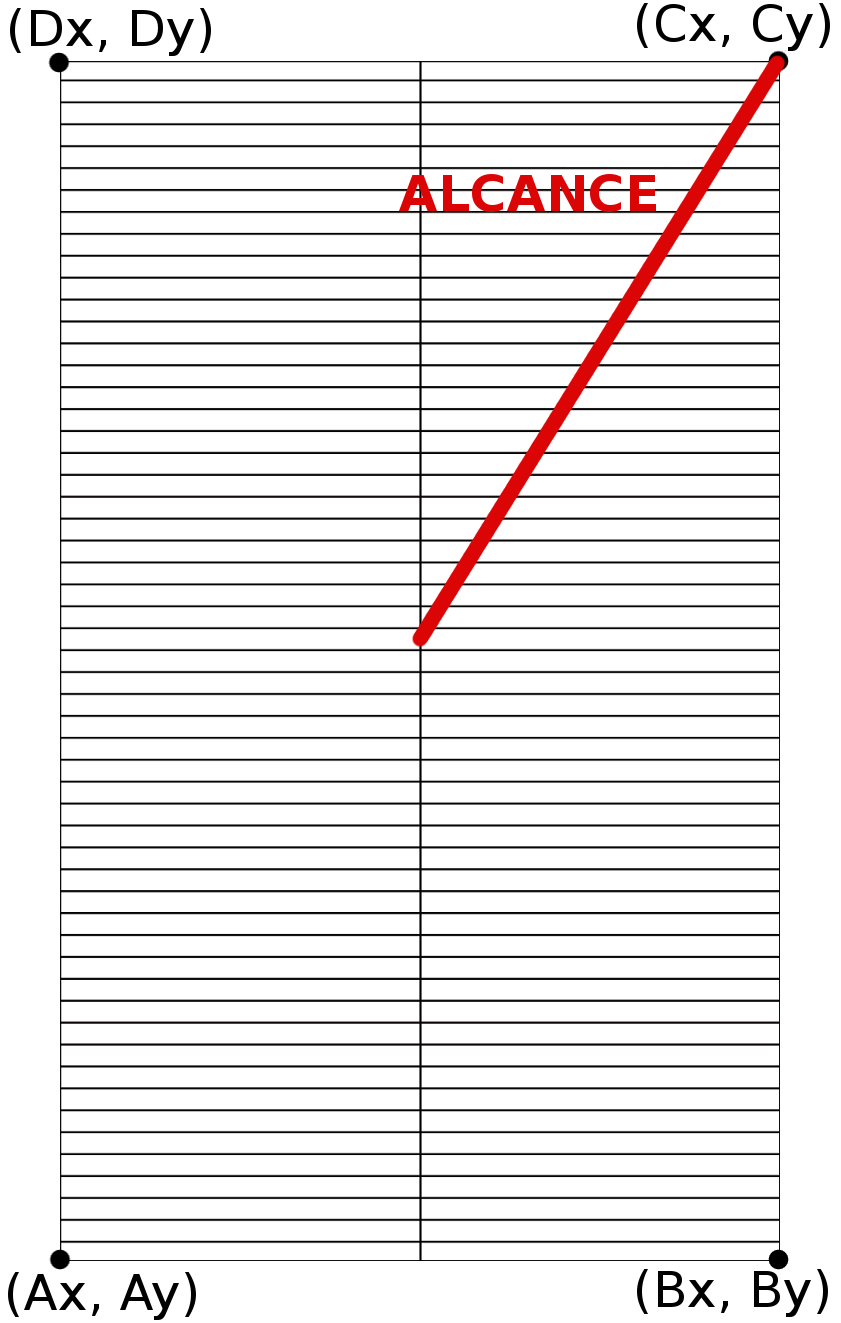
\includegraphics[width=0.5\linewidth]{CSU-vertices}
\caption{Vértices de la CSU}
\label{fig:vertices}
\end{figure}

%%%%%%%%%%%%%%%%%%%%%%%%%%%%%%%
\subsubsection{Métodos relevantes de \texttt{CSU}} \label{subsec:CSUmet}
Uno de los métodos más importantes de esta clase es aquél en el que se decide si
un objeto está dentro o no del apuntado. El método utiliza una simplificación 
del método conocido como ``ray casting'', utilizado en el desarrollo de
videojuegos para determinar colisiones entre polígonos. Este método verifica si
un punto se encuentra situado a la izquierda o a la derecha de uno de los
vértices del polígono. 
En nuestro caso, si un objeto se encuentra a la izquierda
de todas las aristas que forman el rectángulo del apuntado, significa que está
dentro del mismo. 
El código que comprueba esto es la función auxiliar
\texttt{estaDentro2}, que se muestra en el Listado \ref{codigo:csu0}.

\begin{lstlisting}[float=tp,language=C++, basicstyle=\ttfamily\footnotesize,caption={Código del ray casting simplificado},label={codigo:csu0}]                  
#define edge(x1, y1, x2, y2) (-(y2-y1) * p.getx() + (x2 - x1) * p.gety() - (-(y2-y1)*x1 + (x2-x1)*y1))
bool CSU::estaDentro2(const Element &p) const {
  set<Element>::iterator it = puntos.find(p);
  if (it != puntos.end())
    return false;
  register double distancia = (double)sqrt((p.getx() - x) * (p.getx() - x) + (p.gety() -y) * (p.gety() -y));
  if (distancia <= ALCANCE) {
    static int D1, D2, D3, D4;
    D1 = edge(Ax, Ay, Dx, Dy);
    D2 = edge(Dx, Dy, Cx, Cy);
    D3 = edge(Cx, Cy, Bx, By);
    D4 = edge(Bx, By, Ax, Ay);
    return (D1 <= 0 && D2 <= 0 && D3 <= 0 && D4 <= 0);
  }
  return false;
}

\end{lstlisting}

$ALCANCE$ es una constante cuyo valor corresponde a la distancia entre
el centro del apuntado y cualquiera de sus vértices (ver Figura
\ref{fig:vertices}. Si un punto está a una
distancia superior a esa, está fuera del radio de acción de la CSU, por lo que
no podrá estar dentro sea cual sea el ángulo $\alpha$ del apuntado. Si un objeto
se encuentra entre los vértices, se comprueba de que su posición sea válida
respecto a las barras. 
Esto se hace en la función pública \texttt{estaDentro},
cuyo código se muestra en el Listado \ref{codigo:csu1}.

\begin{lstlisting}[float=tp,language=C++,basicstyle=\ttfamily\footnotesize,
                   caption={Función que comprueba si un objeto está en la CSU},
                   label={codigo:csu1}]                  
int CSU::estaDentro(const Element &p, int &barra, double &distancia, double &rango) const {
  static double new_x, new_y, zone;
  if (estaDentro2(p)) {
    testeo(p, new_x, new_y);
    zone = sqrt((Ax - new_x) * (Ax - new_x) + (Ay - new_y) * (Ay - new_y));
	  barra = (int)(zone / DIST_BARRAS);
    if (barra == NUM_BARRAS)
      return 0;
    rango = zone - (barra * DIST_BARRAS);
    distancia = (double)sqrt((p.getx() - new_x) * (p.getx() - new_x) 
                           + (p.gety() - new_y) * (p.gety() - new_y));
    if (distancia > 2*ANCHO)
      return 0;
    if (barras_ocupadas[barra]) 
      return p_potencial(rango, barra);
    //Evitamos que esten justo donde van las barras
    static double redondeo; //demasiada precision en doubles
    redondeo = ceil(rango * PRECISION) / PRECISION;
    if (redondeo < BORDE_INF_DEF || redondeo > BORDE_SUP_DEF){
      return p_potencial(rango, barra);
    }
    //Miramos los bordes (1 arcseg por cada lado)
    if (conf.noborder) 
      if (redondeo <= BORDE_INF || redondeo >= BORDE_SUP)
        return p_potencial(rango, barra);
    if (conf.beamswitching) {
      if (orientacion == ARRIBA) 
        if (redondeo < BARRA2_3)
          return p_potencial(rango, barra);
      if (orientacion == ABAJO)
        if (redondeo > BARRA1_3)
          return p_potencial(rango, barra);
    }
    return !barras_ocupadas[barra];
  }
  return 0;
}
\end{lstlisting}

La función \texttt{testeo} calcula el punto de intersección entre la recta
formada por los vértices A y D de la CSU (lado izquierdo) y un objeto dado.
Cuando el método \texttt{estaDentro} comprueba que el punto coincide
perfectamente con una barra libre, devuelve el valor 1, en caso contrario hace
una llamada al método \texttt{p\_potencial}, que comprueba si el objeto podría
pertenecer al apuntado si se le realizara un mínimo movimiento de ajuste al
mismo. Dicho método devuelve los valores que aparecen en la Tabla
\ref{table:val_posibles}.

\begin{table*}[!ht]
\centering
\begin{tabular}{||l||c|c||}
\hline
\hline
 & Objeto en parte superior & Objeto en parte inferior \\
\hline
\hline
Barra actual libre &  2 & 5 \\
\hline
Barra superior libre & 3 & 0 \\
\hline
Barra inferior libre & 0 & 4 \\
\hline
\hline
\end{tabular}
\caption{Posibles valores del método \texttt{p\_potencial}}
\label{table:val_posibles}
\end{table*}

Los resultados pares indican que se ha de subir el centro del apuntado, de
manera que los objetos ``bajen'', los resultados impares implican lo contrario,
y el valor 0 indica que ese punto no puede pertenecer a la CSU puesto que no ha
superado las condiciones necesarias. Las restricciones que se usan se pueden observar
en el Listado \ref{codigo:csu2}.

\begin{lstlisting}[float=tpb,
                   language=C++,basicstyle=\ttfamily\footnotesize, 
                   caption={Función que comprueba si un objeto podría estár en la CSU},
                   label={codigo:csu2}]
int CSU::p_potencial(const double &rango, int &barra) const {
  if (rango > limiteS) { //Parte superior de la barra
    if (!barras_ocupadas[barra] && rango - limiteS + 0.01 <= margenDown)
      return 2;
    if (barra < NUM_BARRAS-1 && !barras_ocupadas[barra+1])
      if (DIST_BARRAS - rango + limiteI + 0.01 <= margenUp) {
        barra++;
        return 3;
      }
  }
  if (rango < limiteI) { //Parte inferior de la barra
    if (limiteI - rango + 0.01 <= margenUp) {
      if (barras_ocupadas[barra])
        return 0;
      else
        return 5;
    }
    if (barra > 0 && !barras_ocupadas[barra-1])
      if (rango + (DIST_BARRAS-limiteS) + 0.01 <= margenDown) {
        barra--;
        return 4;
      }
  }
  return 0;
}
\end{lstlisting}

Cuando un punto se ajusta perfectamente con una barra y no hay que mover el apuntado,
se utiliza el método \texttt{pointAdd}, que comprueba los límites y márgenes
del apuntado respecto al nuevo punto, lo introduce en el conjunto de puntos que
componen el apuntado y marca la barra en la que se encuentra como ocupada. Sin
embargo, cuando hay que hacer ajustes mínimos para que el objeto pueda ser
introducido, se utiliza la función \texttt{pointAddMove}, cuya implementación se
muestra en el Listado \ref{codigo:csu3}.

\begin{lstlisting}[float=tpb,
                   language=C++,basicstyle=\ttfamily\footnotesize,
                   caption={Método que añade un punto que requiere de ciertos ajustes},
                   label={codigo:csu3}]
void CSU::pointAddMove(Element &p, const int &move) {
  static double dist;
  if (move == 2 || move == 4) { //Hay que subir la CSU
    if (move == 2) //esta muy arriba
      dist = p.getzona() - limiteS + 0.01;
    if (move == 4)  //pasar a barra inferior
      dist = p.getzona() + (DIST_BARRAS - limiteS) + 0.01;
    if (alfa == CERO) { //es vertical, subimos la Y
      y += dist;
    }
    else if (alfa == PIMEDIO) { //es horizontal, movemos la X
      x -= dist;
    }
    else {
      static double raiz;
      raiz = sqrt((dist*dist)/(1 + ma * ma));
      y -= ma * raiz;
      x -= raiz;
    }
    margenDown -= dist;
    margenUp += dist;
  }
  else { //Hay que bajar la CSU
    if (move == 3)  //Pasar a barra superior 
      dist = DIST_BARRAS - p.getzona() + limiteI + 0.01;
    if (move == 5) { //Esta demasiado abajo
      dist = limiteI - p.getzona() + 0.01;
    }
    if (alfa == CERO) { //es vertical, bajamos la Y
      y -= dist;
    }
    else if (alfa == PIMEDIO) { //es horizontal, movemos la X
      x += dist;
    }
    else {
      static double raiz;
      raiz = sqrt((dist*dist)/(1 + ma * ma));
      y += ma * raiz;
      x += raiz;
    }
    margenDown += dist;
    margenUp -= dist;
  }
  extremos();
  puntos.insert(p);
  barras_ocupadas[p.getbarra()] = true;
  if (p.getprior() < prior)
    prior = p.getprior();
  actualizar2();
}
\end{lstlisting}

En la función \texttt{pointAddMove} se calcula cuál es la distancia mínima necesaria para que el
objeto pueda ser introducido, dependiendo de la opción en la que se encuentre el
mismo (véase la Tabla \ref{table:val_posibles}). Una vez movido el centro de la
\texttt{CSU} se invocan dos métodos muy importantes de esta clase. El primero,
\texttt{extremos}, recalcula la posición de los vértices del apuntado, puesto
que se ha movido de sitio; y el segundo, \texttt{actualizar2}, se encarga de
comprobar de nuevo todos aquellos atributos que dependen de la posición de los
objetos, tales como las distancias mínimas recogidas en el atributo
\texttt{distancia\_punto} o los nuevos márgenes de movimiento del apuntado.

En el Capítulo \ref{chap:algorithm} se hacía referencia a una serie de movimientos de mejora
que se podían efectura sobre la \texttt{CSU}, con el objetivo de abarcar un mayor número de objetos.
Estos posibles movimientos son cuatro y se agrupan en dos: movimientos
verticales y movimientos horizontales. En los primeros, se produce un cambio de
barra de los objetos, situando aquél que se encuentre en la barra más cercana al
borde inferior de la \texttt{CSU} en la barra 0 del apuntado (en el caso de la mejora
hacia arriba) o trasladando el objeto que ocupa la barra más cercana al borde
superior en la última barra (en el otro caso). En este tipo de movimiento la
zona de la barra en la que se encuentra un objeto no se ve afectada. Por el
contrario, en el segundo tipo de movimiento, el horizontal, lo que no se ve
afectado es la barra de cada uno. En este caso lo que se persigue es mover los
objetos hasta el borde izquierdo o derecho del apuntado, obteniendo una nueva
área de búsqueda alrededor de la \texttt{CSU}. Nuevamente se ha de llamar al método
\texttt{extremos} para calcular los nuevos vértices del apuntado con cada
movimiento. En el Listado \ref{codigo:csu4} se muestra un ejemplo de cada uno de
los tipos de mejora mencionados.

\begin{lstlisting}[float=tpb,
                   language=C++, basicstyle=\ttfamily\footnotesize, 
                   caption={Código del movimiento de mejora vertical hacia arriba},
                   label={codigo:csu4}]
void CSU::mejoraArriba() {
  static int i, j, z;
  static double dist;
  i = CERO;
  while (!barras_ocupadas[i])
    i++;
  if (i != CERO) {
    for (j = CERO; j+i < NUM_BARRAS; j++){
      barras_ocupadas[j] = barras_ocupadas[j+i];
    }
    for (j = NUM_BARRAS - i; j < NUM_BARRAS; j++){
      barras_ocupadas[j] = false;
    }
    dist = i * DIST_BARRAS;
    if (alfa == CERO) { //es vertical, subimos la Y
      y += dist;
    }
    else if (alfa == PIMEDIO) { //es horizontal, movemos la X
      x -= dist;
    }
    else {
      static double raiz;
      raiz = sqrt((dist*dist)/(1 + ma * ma));
      y -= ma * raiz;
      x -= raiz;
    }
    extremos();
    actualizar(-i);
  }
}
\end{lstlisting}

\begin{lstlisting}[float=tpb,
                   language=C++, basicstyle=\ttfamily\footnotesize,
                   caption={Código del movimiento de mejora horizontal izquierdo},
                   label={codigo:csu5}]
void CSU::mejoraIzquierda() {
  static int j;
  static double dist;
  if (dist_min > 0.2) {
  dist = dist_min - 0.1;
  if (alfa == CERO) { //es vertical, movemos la X
    x += dist;
  }
  else if (alfa == PIMEDIO) { //es horizontal, movemos la Y
    y += dist;
  }
  else {
    static double raiz;
    raiz = sqrt((dist*dist)/(1 + mb * mb));
    if (alfa < PIMEDIO) {
      x += raiz;
      y += mb * raiz;
    } else {
      x -= raiz;
      y -= mb * raiz;
    }
  }
  extremos();
  actualizar(0);
  }
}
\end{lstlisting}

En ambos casos se utiliza la función \texttt{actualizar}, que funciona de modo
análogo a \texttt{actualizar2}, actualizando los objetos y el contenido de los
atributos.

El método \texttt{colision} es otra de las claves de esta clase, pues se encarga
de determinar si entre dos apuntados existe una colisión o solape. La forma de
comprobarlo es mediante proyecciones de planos e intersecciones de rectas: se
proyectan los vértices de una \texttt{CSU} $B$ sobre las rectas definidas por
los vértices AD y AB de la \texttt{CSU} $A$. Si en alguna de estas proyecciones
el rango dado por el par de vértices (mínimo y máximo) proyectados no tiene
puntos en común con el rango formado por el par de vértices AD, o AB según el
caso, podemos afirmar que no hay colisión. En caso de no poder realizar tal
afirmación, comprobamos si existe algún punto de $A$ en $B$, en cuyo caso se
afirmaría que existe un solapamiento entre ambas. Se debe tener en cuenta que
aunque se llegue al final del método y no haya ningún punto de $A$ en $B$, es
posible que sí haya alguno de $B$ en $A$, por lo que se debe hacer doble
comprobación. El código de este método se muestra en el Listado
\ref{codigo:csu6}.

\begin{lstlisting}[float=tpb,
                   language=C++, basicstyle=\ttfamily\footnotesize, numbers=none,
                   caption={Código del método que comprueba las colisiones},
                   label={codigo:csu6}]
bool CSU::colision (const CSU &csu) const {
  csu.getABCD(s2);  //Ax,Ay,Bx,By,Cx,Cy,Dx,Dy
  //RECTA AD
  for (i = 0; i < 8; i+=2) { //cada uno de los puntos de CSU2
    if (alfa != CERO && alfa != PIMEDIO) { // No es ni vertical ni horizontal
      punto.first = (ma * Ax - mb * s2[i] + s2[i+1] - Ay) / (ma - mb);
      punto.second = ma * (punto.first - Ax) + Ay;
    }
    else if (alfa == CERO){   // Es vertical
      punto.first = Ax;
      punto.second = s2[i+1];
    }
    else{  // Es horizontal
      punto.first = s2[i];
      punto.second = Ay;
    }
    minimoX = min(minimoX, punto.first);
    maximoX = max(maximoX, punto.first);
    minimoY = min(minimoY, punto.second);
    maximoY = max(maximoY, punto.second);
  }
  //Comprobamos que no haya solape
  miX = min(Ax,Dx); maX = max(Ax,Dx);
  if (maximoX < miX)
    return false;
  if (minimoX > maX)
    return false;
  miX = min(Ay,Dy); maX = max(Ay,Dy);
  if (maximoY < miX)
    return false;
  if (minimoY > maX)
    return false;
  //Repetimos para el lado DC
  //Comprobamos si los puntos colisionan
  CSU vacia (csu.getx(), csu.gety(), csu.getalfa());
  for (p = puntos.begin(); p != puntos.end(); p++)
    if (vacia.estaDentro(*p,b,d,z))
      return true;
  return false;
}
\end{lstlisting}
%%%%%%%%%%%%%%%%%%%%%%%%%%%%%%%
\subsection{La clase \texttt{Parser}}
\texttt{Parser} hereda de la clase \texttt{SaxParser}, definida en la librería
\texttt{libxml++}, cuya función es actuar como un parser de XML. 
\texttt{Parser} es una adaptación a nuestro problema particular de los métodos que aparecen en la
documentación de la librería. Sus objetivos son los de comprobar que la
estructura del fichero de entrada a \CSUO{} sea el correcto y devolver los
datos contenidos en dicha entrada en las estructuras explicadas anteriormente.
La estructura del fichero de entrada es la que se muestra en el Listado
\ref{codigo:xml-in}.

\begin{lstlisting}[float=tpb,
                   numbers=none,
                   language=XML,
                   caption={Estructura de los ficheros de entrada para \CSUO{}},
                   label={codigo:xml-in}]
<Observables [widht=``Ancho_cielo'' height=``Alto_cielo'']>
    <Element id=``Identificador''>
        <X>PosX</X>
        <Y>PosY</Y>
        <Prioridad>[1..99]</Prioridad>
    </Element>
<!-- ...  -->
</Observables>
\end{lstlisting}

En el Listado \ref{codigo:xml-exacto} se muestra un extracto de un ejemplo de entrada con datos
reales, extraídos del fichero \texttt{exacto.xml}.

\begin{lstlisting}[float=tpb,
                   numbers=none,
                   language=XML,
                   caption={Ejemplo de entrada para \CSUO{},
                   extraído de \texttt{exacto.xml}},
                   label={codigo:xml-exacto}]
<Observables widht="900" height="900">
	<Element id="0">
		<x>573</x>
		<y>402.4242</y>
		<Prioridad>1</Prioridad>
	</Element>
	<Element id="1">
		<x>595</x>
		<y>409.6968</y>
		<Prioridad>1</Prioridad>
	</Element>
	<Element id="2">
		<x>458</x>
		<y>416.9694</y>
		<Prioridad>1</Prioridad>
	</Element>
	<Element id="3">
		<x>409</x>
		<y>424.242</y>
		<Prioridad>1</Prioridad>
	</Element>
<!-- ...  -->
	<Element id="54">
		<x>409</x>
		<y>795.1446</y>
		<Prioridad>1</Prioridad>
	</Element>
</Observables>
\end{lstlisting}

Los datos facilitados a la aplicación han de estar en arcosegundos, y nunca con
valores negativos. 
En caso de tener una instancia de entrada que no cumpla este requisito puede
utilizarse el conversor que se explica en la Sección \ref{sec:conver}.

%%%%%%%%%%%%%%%%%%%%%%%%%%%%%%%
\subsubsection{Atributos de \texttt{Parser}}
\begin{itemize}
\item \texttt{Q}: conjunto de objetos contenidos en el fichero de entrada.
\item \texttt{fich}: fichero XML de entrada.
\item \texttt{punto}: objeto donde se crean las instancias de los elementos
contenidos en el archivo entrante.
\item \texttt{nodo}: identificador del  nodo en el que se encuentra el
analizador durante el procesado.
\item \texttt{nuevo}: indica el nivel de procesado que lleva en la estructura,
en nuestro caso cuando llega a 3 se determina que ha completado un elemento.
\item \texttt{widht, height}: ancho y alto especificados para definir el tamaño
de la pantalla de Allegro.
\end{itemize}
%%%%%%%%%%%%%%%%%%%%%%%%%%%%%%%
\subsubsection{Métodos relevantes de \texttt{Parser}}
Cuando se construye una instancia de esta clase comienza el procesado del
archivo especificado por parámetro. En el constructor se comprueba línea a línea
si el fichero sigue la estructura especificada, mediante llamadas a las funciones
virtuales de la clase. Éstas son métodos que especifican qué se comprueba en
cada nivel y cuando se ha terminado de construir un objeto para añadirlo a
\texttt{Q}. El método que realmente interesa es \texttt{getList}, que
devuelve el conjunto de datos de entrada del problema.

%%%%%%%%%%%%%%%%%%%%%%%%%%%%%%%
\subsection{La clase \texttt{Dbscan}} \label{sec:dbscan}
Esta es la clase que implementa el algoritmo descrito en la Sección
\ref{sec:clustering}. El código de \texttt{Dbscan} es el resultado de una
adaptación y traducción a C++ de un código Java que implementaba este algoritmo de clustering.
Se ha mantenido el tipo de los atributos para evitar alterar el correcto
funcionamiento del código. 

Los objetos (de la clase \texttt{Element}) se agrupan en vectores, definidos en
la clase estándar \texttt{vector} de C++. 
Este contenedor agrupa los objetos por orden de llegada. 

%%%%%%%%%%%%%%%%%%%%%%%%%%%%%%%
\subsubsection{Atributos de \texttt{Dbscan}}
\begin{itemize}
\item \texttt{e}: indica la distancia utilizada en el cálculo de vecindades.
\item \texttt{minpt}: mínimo de puntos que forman un núcleo.
\item \texttt{resultList}: vector de listas de vectores de elementos. Cada lista
representa un clúster de puntos.
\item \texttt{pointList}: es el conjunto de datos de entrada.
\end{itemize}
%%%%%%%%%%%%%%%%%%%%%%%%%%%%%%%
\subsubsection{Métodos relevantes de \texttt{Dbscan}}
Se utiliza \texttt{setList} y \texttt{getList} para establecer u obtener el
conjunto de objetos de entrada, y el método \texttt{start} para comenzar el
proceso de agrupamiento de los objetos. Para obtener el vector de resultados,
contenido en el atributo \texttt{resultList} se usa el método
\texttt{getResult}.
%%%%%%%%%%%%%%%%%%%%%%%%%%%%%%%
\subsection{Algoritmos principales}

El archivo \texttt{main.C} organiza el uso de todas las clases descritas para
implementar el algoritmo constructivo planteado en la Sección
\ref{sec:algconst}. El código para crear la solución inicial de dicho algoritmo
es el que se presenta en el Listado \ref{codigo:main1}.

\begin{lstlisting}[float=tpb,
                   language=C++, numbers=none,
                   caption={Primera fase del algoritmo constructivo: generar la solución inicial},
                   label={codigo:main1}]
set<CSU> diferentes[5];
sort(diferentes[0],TAMPUN);
int mej, min = MAX;
CLOCK_Start(chrono);
for (int i = MENORX; i < 5; i++) {
  diferentes[i] = apuntadosRandom(parser.getList(), i);
  if (diferentes[i].size() < min) {
    min = diferentes[i].size();
    mej = i;
  }
}
set<CSU> centros = diferentes[mej];
\end{lstlisting}

En el Listado \ref{codigo:main2} se detalla la función \texttt{apuntadosRandom},
encargada de generar varias soluciones del problema sobre las que se elige la
mejor.

\begin{lstlisting}[float=tpb,
                   language=C++, numbers=none,basicstyle=\ttfamily\footnotesize,
                   caption={Código de la función que genera soluciones
                   aleatorias},
                   label={codigo:main2}]
set<CSU> apuntadosRandom(set<Element> puntos, const int &opcion) {
  static set<Element>::iterator v;
  static set<CSU> posibles;
  set<CSU> resultado;
  posibles.clear();
  static set<CSU>::iterator i;
  static CSU mejor_opcion;
  static int contador;
  if (opcion <= 4) {
    sort(puntos, opcion);
    set<Element> eliminados;
    set<Element> cluster = puntos;
    static set<Element>::iterator e1;
    while (!puntos.empty()) 
      for (v = cluster.begin(); v != cluster.end(); v++) { 
        progreso();
        e1 = eliminados.find(*v);
        if (e1 == eliminados.end()) {
          posibles = selectAP(*v, puntos);
          i = posibles.begin(); 
          mejor_opcion = *i; 
          resultado.insert(mejor_opcion);
          eliminar_puntos(mejor_opcion.getPoints(), puntos, eliminados); 
        }
      }
  }
	// ... //
  return resultado;
}
\end{lstlisting}

La segunda fase, en la que se realiza el proceso de eliminar solapes entre
apuntados, se realiza dentro de \texttt{colisiones}. Este método se encuentra
detallado en el Apéndice \ref{app:colis} debido a su extensión.

La implementación del algoritmo \texttt{GRASP} definido en la Sección
\ref{sec:grasp} se encuentra en la función \texttt{grasp} del fichero
\texttt{main.C}, mostrada en el Apéndice \ref{app:grasp}.

%%%%%%%%%%%%%%%%%%%%%%%%%%%%%%%
\section{Modo de empleo de \CSUO{}} \label{sec:uso_app}

Para utilizar \CSUO{} una vez compilada (usando \texttt{make}),
hay que especificar una serie de opciones y un archivo \texttt{XML} con los
objetos de entrada.

\begin{lstlisting}[numbers=none]
$ ./csuoptimizer [opciones] entrada.xml
\end{lstlisting}

Las opciones disponibles en \CSUO{} son: 
\begin{itemize}
\item \texttt{--help}: Muestra una ayuda con las opciones disponibles y un
ejemplo de uso.
\item \texttt{--dbscan}: indica a \CSUO{} que se quiere hacer uso
del algotimo DBScan explicado en la Sección \ref{sec:dbscan}. Desactivado por
defecto.
\item \texttt{--grasp}: habilita el uso de la heurística GRASP para intentar
mejorar la solución. Desactivada por defecto.
\item \texttt{--graphic}: muestra en la ventana generada por Allegro los pasos
que está realizando \CSUO{} durante su ejecución. Este paso está
pensado para labores de depuración y desarrollo y ralentiza la ejecución de la
aplicación.
\item \texttt{-NR}: especifica el número de rotaciones que hará una CSU durante
el proceso de búsqueda de objetos inicial. Por defecto este valor es igual a 20,
pues se han obtenido buenos resultados en todos los ejemplos. Un ejemplo de su
uso sería \texttt{./csuoptimizer -NR 15 entrada.xml}.
\item \texttt{--verbose}: genera un archivo \texttt{verbose.txt} con información
de control, útil para depuración y desarrollo.
\item \texttt{--dat}: indica el modo de salida de los resultados. Por defecto se
usa el formato \texttt{XML}, cuyo ejemplo se puede ver en el Anexo
\ref{app:exacto.xml}, sin embargo es posible que el usuario requiera de otro
tipo de salida. Esta estructura adicional se muestra en el Listado
\ref{codigo:exacto.dat}.
\item \texttt{--beams}: habilita el uso del \texttt{beam switching}.
\item \texttt{--noborder}: especifica que no se quieren objetos cercanos a la
barra, por lo que se deshabilita un espacio de 1 arcosegundo en cada uno de los
bordes.
\end{itemize}


\begin{lstlisting}[float=tpb,
                   numbers=none,mathescape,
                   caption={Estructura del modo de resultado \texttt{.dat}},
                   label={codigo:exacto.dat}]
**************************************************************
coordenadaX			coordenadaY			anguloInclinacion
				posicionBarra_1
				posicionBarra_2

				   $\vdots$

				posicionBarra_55
**************************************************************
coordenadaX			coordenadaY			anguloInclinacion

    $\vdots$

\end{lstlisting}

Las opciones \texttt{--beams} y \texttt{--noborder} afectan al área útil de una
barra. En la Figura \ref{fig:barras} se muestran los casos posibles de una
barra. La zona blanca es la zona útil de barra, donde se puede detectar un
objeto, la zona en color gris hace referencia al área eliminada por el usuario
mediante las opciones.

\begin{figure}[!htb]
\centering
\subfloat{

\includegraphics[width=0.2\linewidth]{BarraPunto1}}
\subfloat{

\includegraphics[width=0.2\linewidth]{BarraPunto2}}
\subfloat{

\includegraphics[width=0.2\linewidth]{BarraPunto3}}
\subfloat{

\includegraphics[width=0.2\linewidth]{BarraPunto4}}
\caption{Disponibilidad de las barras según las opciones de entrada. a) Barra
normal. b) Barra con \texttt{--noborder}. c) Barra con \texttt{--beams}. d)
Barra con ambas opciones}
\label{fig:barras}
\end{figure}

%%%%%%%%%%%%%%%%%%%%%%%%%%%%%%%
\section{Herramientas de apoyo}
Con el objetivo de comprobar el buen funcionamiento de \CSUO{} y
de facilitar al usuario herramientas útiles que permitan una mayor
familiarización con la aplicación, se aportan dos herramientas complementarias
explicadas en las siguientes Secciones.
%%%%%%%%%%%%%%%%%%%%%%%%%%%%%%%
\subsection{``Editor de mapas''}
En el directorio \texttt{map\_editor} del proyecto se encuentra un programa \texttt{mapEditor} que
genera entradas para el \CSUO{} con apuntados específicos. 
Los ejemplos sintéticos que se presentan en la Sección \ref{sec:sintetico} de esta
Memoria han sido generados mediante esta aplicación. Se cuenta con un archivo
\texttt{Makefile} para automatizar la compilación.

El \texttt{mapEditor} generado por la compilación muestra un menú por consola
con las siguientes opciones:
\begin{itemize}
\item \texttt{1 Crear CSU}: permite especificar la posición de una CSU así como
su ángulo de inclinación. Automáticamente se añade un objeto en cada barra de
forma aleatoria. La pantalla gráfica de esta aplicación tiene un tamaño de
$900\times900$ arcosegundos, por lo que se deben introducir valores en este
rango para poder visualizarlos.
\item \texttt{2 Visualizar CSUs}: muestra la disposición de las CSUs en el
espacio visible.
\item \texttt{3 Visualizar Puntos}: muestra únicamente la nube de objetos
generada, la cual será la entrada a la aplicación \CSUO{}.
\item \texttt{4 Visualizar Espacio}: muestra de manera conjunta las dos opciones
anteriores, es decir, cada apuntado con sus respectivos objetos.
\item \texttt{5 Guardar puntos}: genera un archivo \texttt{XML} con los objetos
creados, el cual será el fichero de entrada de \CSUO{}.
\item \texttt{6 Salvar datos}: guarda el estado actual de la aplicación en un
fichero \texttt{save.dat} para reutilizarlo cuando convenga.
\item \texttt{7 Cargar datos}: carga en memoria un estado antiguo de la
aplicación desde un fichero especificado por el usuario.
\end{itemize}
%%%%%%%%%%%%%%%%%%%%%%%%%%%%%%%
\subsection{Conversor} \label{sec:conver}
Los ejemplos facilitados por el responsable del proyecto EMIR no se presentan en
el formato de entrada requerido por \CSUO{}, razón por la que se ha
incluido un conversor que:
\begin{itemize}
\item transforma un fichero con datos en texto plano agrupados por columnas (véase
el Listado \ref{codigo:estructdat}) al formato de entrada requerido.
\item realiza un cambio de coordenadas para evitar valores negativos en
\CSUO{}.
\item permite cambiar de grados a arcosegundos con la opción \texttt{-g2a}.
\end{itemize}

Esta herramienta genera dos archivos de salida:
\begin{itemize}
\item Uno con la misma estructura que la entrada, es decir, la que se muestra en
el Listado \ref{codigo:estructdat}, terminado en \texttt{-converted.dat} en
\texttt{ejemplos/} para que se tenga un control de cambios en los objetos debido
al cambio del centro de origen.
\item Un fichero con el mismo nombre que el de origen pero en XML situado en
\texttt{ejemplos/xml/} listo para su uso en \CSUO{}.
\end{itemize}

Ejemplo de uso:
\begin{lstlisting}[float=tpb,
                   numbers=none]
./conversor-dat-xml [-g2a] archivo.dat
\end{lstlisting}

\begin{lstlisting}[caption={Estructura de entrada de los ficheros .dat},
                  label={codigo:estructdat}]
posicionXobjeto1  posicionYobjeto1  prioridadObjeto1
posicionXobjeto2  posicionYobjeto2  prioridadObjeto2

      ...               ...               ....

posicionXobjetoN  posicionYobjetoN  prioridadObjetoN
\end{lstlisting}

%
% ---------------------------------------------------
%
% Proyecto Final de Carrera: EMIR
% Autor: Pedro Hernández Martín <alu3679@etsii.ull.es>
% Capítulo: Estado del arte
% Fichero: Cap2_estado_del_arte.tex
%
% ----------------------------------------------------
%

\chapter{Resultados} \label{chap:resultados}
En este capítulo se presentan los resultados obtenidos con diversas
distribuciones de objetos, tanto generadas de forma sintética y ex-profeso para
comprobar la aplicación, como correspondientes a casos reales. Todos estos
ejemplos se incluyen en el directorio \texttt{ejemplos/} de la aplicación.

Los resultados se muestran en tablas que recogen el número de CSUs que
constituye la solución junto al tiempo (en minutos y segundos) que ha tardado en calcularse la misma,
dependiendo de las opciones que se utilicen en la ejecución. Las opciones se
muestran a la izquierda, por filas, mientras que el tipo de resultado se muestra
en la parte superior, en las columnas.

También se muestran pares de imágenes, correspondientes a la entrada y la salida
(sin especificación de ningún tipo de parámetros adicionales) del programa, para
facilitar la comprensión del ejemplo. La figura de la izquierda representa la
nube de objetos sobre la que el \CSUO{} va a buscar los apuntados, y la
figura de la derecha muestra el resultado obtenido. Se dibuja de un color
diferente cada apuntado para facilitar su diferenciación.

Para los cálculos se ha utilizado una máquina virtual con Ubuntu 12.04 LTS, dos
procesadores y 2 GB de memoria RAM, que corre bajo un Windows 7 nativo, con un
Intel i7 920 (2.67 GHz) y 6 GB de memoria RAM DDR3.

\section{Ejemplos sintéticos} \label{sec:sintetico}
Son ejemplos generados por el ``editor de mapas'' (\texttt{mapEditor}) para depurar la aplicación y
comprobar su comportamiento. Algunas de las distribuciones se generaron de forma
aleatoria, por lo que no hay manera de saber si los resultados son óptimos o
no. Otros ejemplos se han generado siguiendo un patrón concreto, para el que
conocemos de antemano la solución óptima. Para ello situamos en el espacio de
trabajo una CSU ``virtual'' sobre la que colocamos un cierto número de objetos
distribuidos de tal modo que sabemos que ajustan perfectamente con las barra de
esta CSU ``virtual''.
Si el \CSUO{} realiza correctamente su trabajo, colocará una CSU (apuntado) configurado
exactamente igual que la CSU ``virtual'' que ubicamos con el \texttt{mapEditor}.

\subsection {Ejemplo: \texttt{exacto.xml}}
Este ejemplo consiste en 55 objetos a observar distribuidos de forma que cada
uno de ellos ajuste perfectamente dentro de una barra de la CSU, siendo el
resultado óptimo un único apuntado. Al tratarse de un ejemplo creado con el ``editor de
mapas'' la distancia de cada punto es la necesaria para que el resultado no
varíe entre las diversas opciones que se permiten.

%%%%%%%%%%%%%%%%%%%%% Fig. %%%%%%%%%%%%%%%%%%%%%%%%%%%%%%%%%%%
%\begin{figure}[ht]
%\centering
%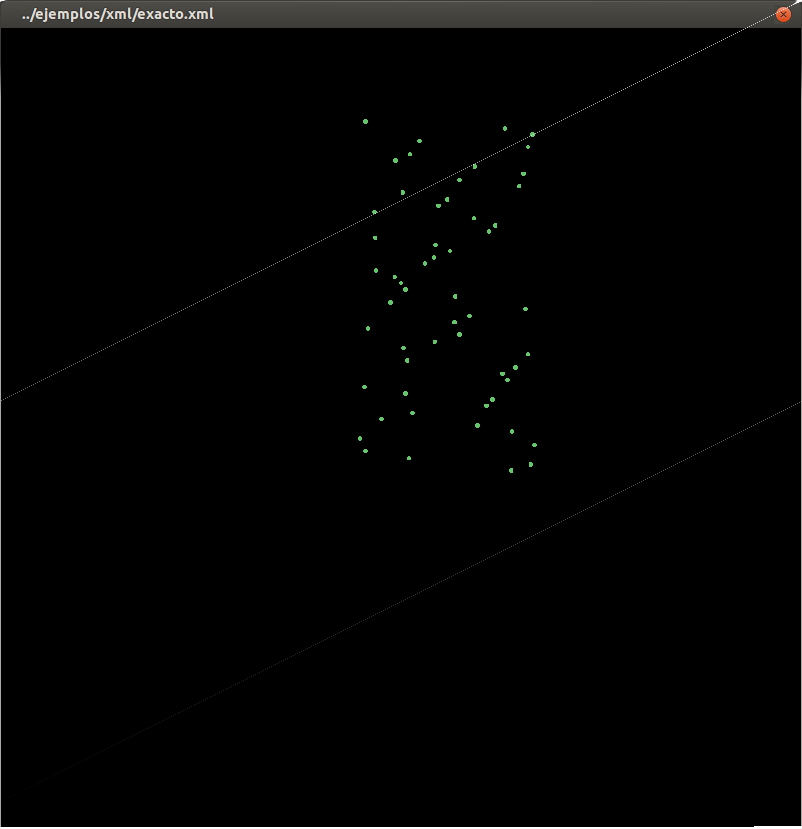
\includegraphics[height=7.5cm]{exacto-in} 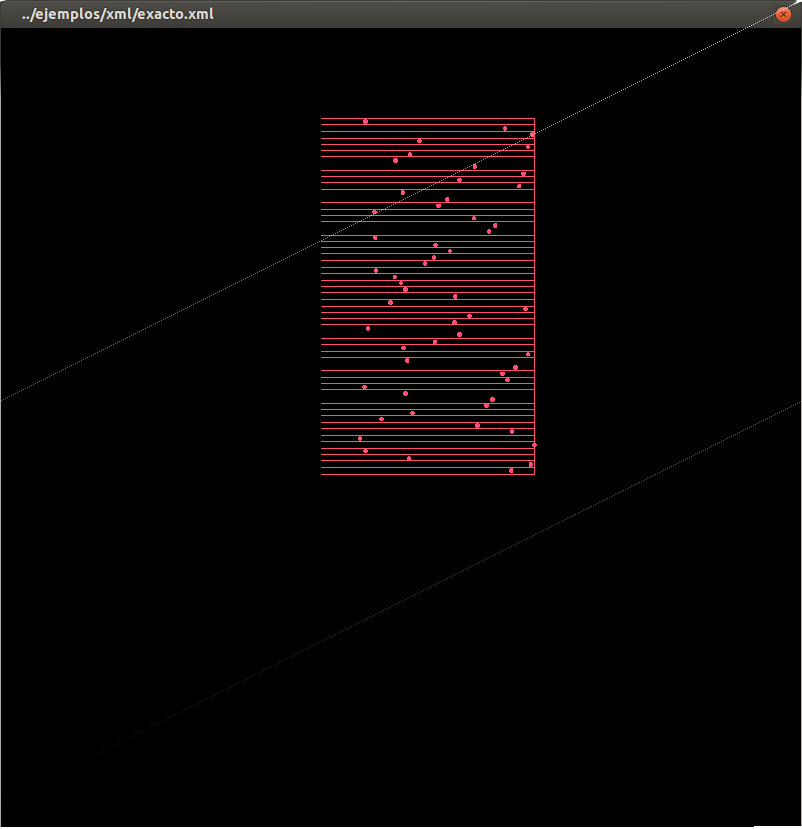
\includegraphics[height=7.5cm]{exacto-out}
%\caption{Ejemplo \texttt{exacto.xml}. 55 objetos que se ajustan perfectamente a una única CSU}
%\label{fig:3rodinia}
%\end{figure}
%%%%%%%%%%%%%%%%%%%%%%%%%%%%%%%%%%%%%%%%%%%%%%%%%%%%%%%%%%%%%

%%%%%%%%%%%%%%%%%%%% Fig. %%%%%%%%%%%%%%%%%%%%%%%%%%%%%%%%%%%
\begin{figure}[!htb]
\centering
\subfloat[Entrada]{
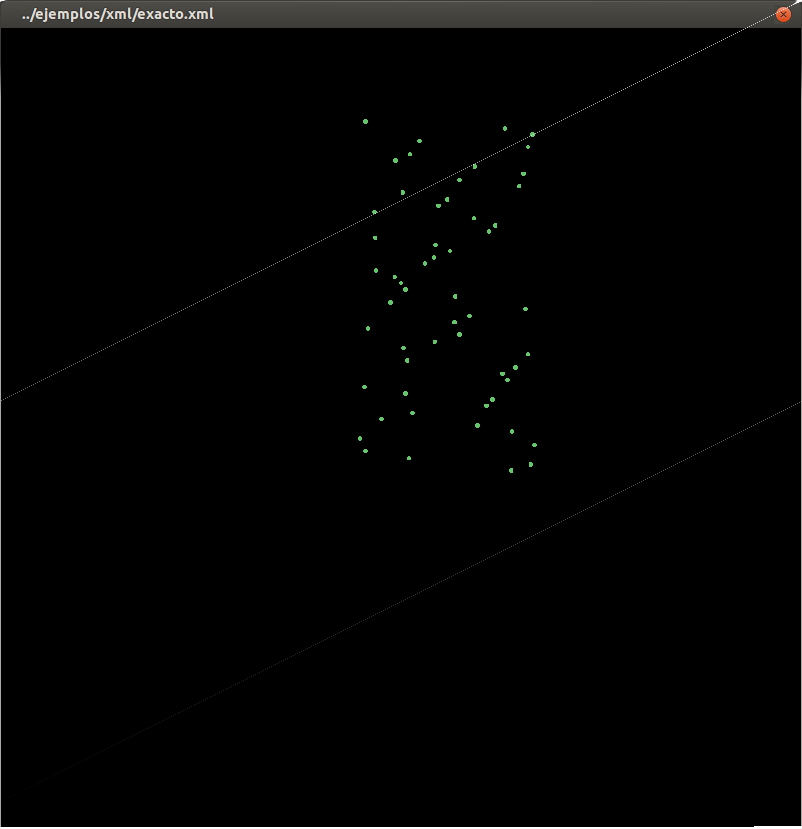
\includegraphics[width=0.5\linewidth]{exacto-in}
\label{fig:exacto-in}}
\subfloat[Salida del \CSUO{}]{ 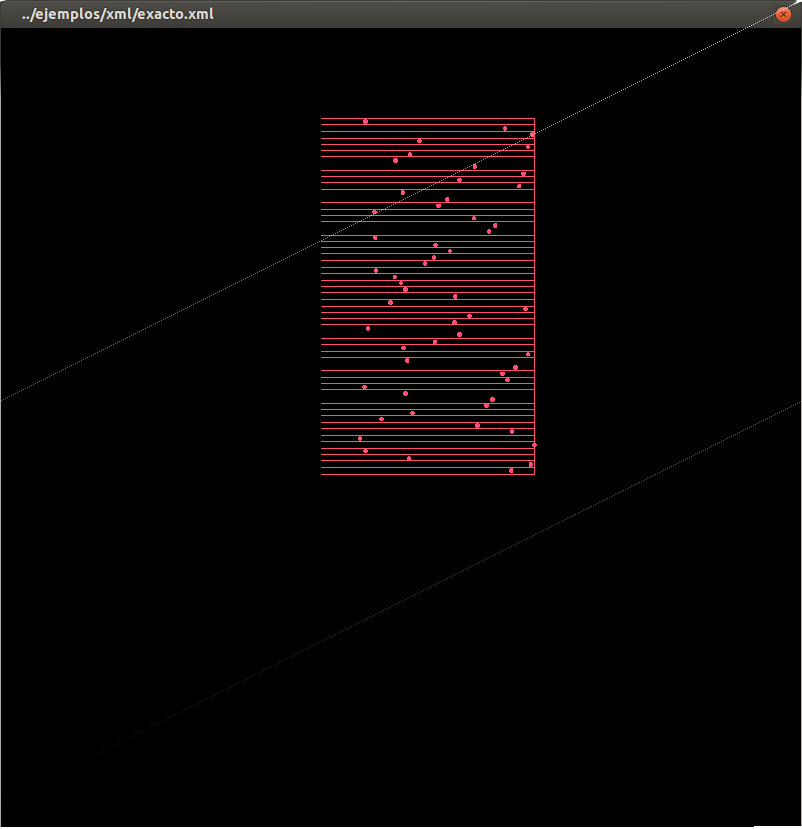
\includegraphics[width=0.5\linewidth]{exacto-out}
\label{fig:exacto-out}}
\caption{Ejemplo \texttt{exacto.xml}. 55 objetos que se ajustan perfectamente a una única CSU}
\end{figure}
%%%%%%%%%%%%%%%%%%%%%%%%%%%%%%%%%%%%%%%%%%%%%%%%%%%%%%%%%%%%%%
\begin{table*}[!ht]
\centering
\begin{tabular}{||l||c|c||}
\hline
\hline
RESULTADOS & Apuntados & Tiempo \\
\hline
\hline
Sin opciones & 1 & 1.02'' \\
\hline
Sin bordes & 1 & 0.76'' \\
\hline
Beam Switching & 1 & 0.72'' \\
\hline
Sin bordes + Beam S. & 1 & 0.89'' \\
\hline
\hline
\end{tabular}
\caption{Resultados del ejemplo \texttt{exacto.xml}}
\end{table*}

El resultado es justamente el esperado, por lo que comprobamos que la aplicación es capaz
de ajustar correctamente un apuntado de manera óptima para este tipo de instancias de entrada.

\subsection {Ejemplo: \texttt{4\_0solapes.xml}}
Este ejemplo consta de 220 objetos, que corresponden a cuatro apuntados
generados de forma que ninguno de ellos se solape con otro, con lo que el
resultado esperado son cuatro apuntados.

%%%%%%%%%%%%%%%%%%%% Fig. %%%%%%%%%%%%%%%%%%%%%%%%%%%%%%%%%%%
\begin{figure}[!htb]
\centering
\subfloat[Entrada]{
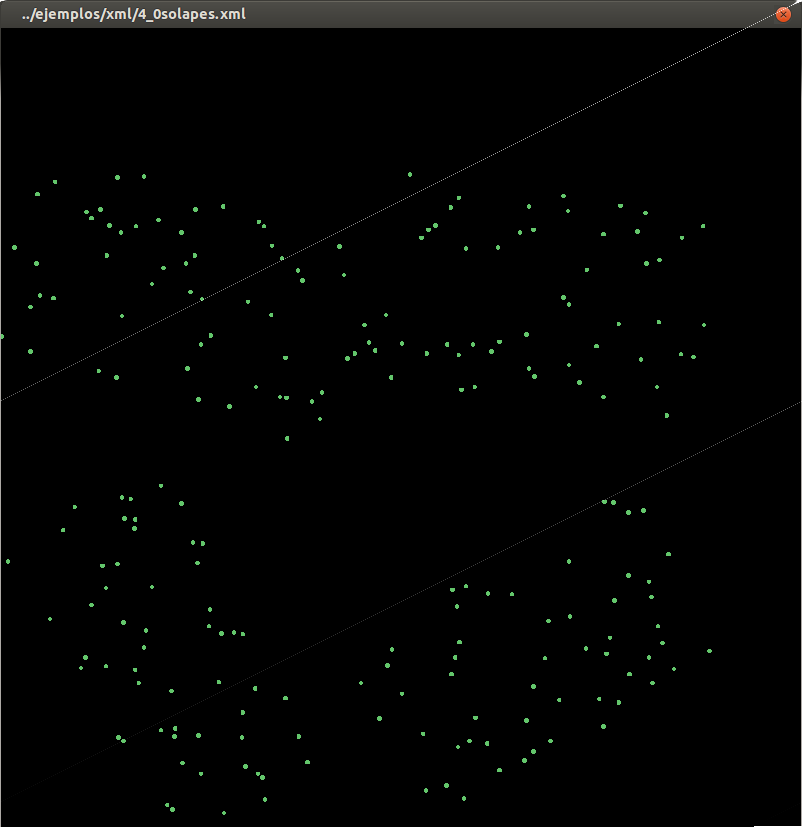
\includegraphics[width=0.5\linewidth]{4_0solapes-in}
\label{fig:4_0solapes-in}}
\subfloat[Salida del \CSUO{}]{
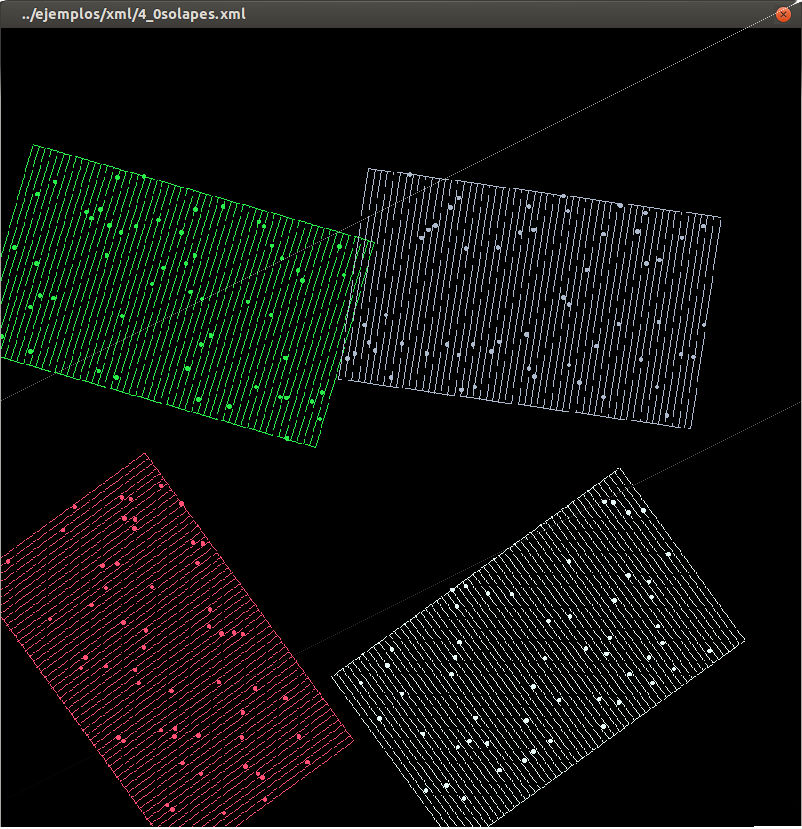
\includegraphics[width=0.5\linewidth]{4_0solapes-out}
\label{fig:4_0solapes-out}}
\caption{Ejemplo \texttt{4\_0solapes.xml}. 4 apuntados distanciados entre si}
\end{figure}
%%%%%%%%%%%%%%%%%%%%%%%%%%%%%%%%%%%%%%%%%%%%%%%%%%%%%%%%%%%%%%

\begin{table*}[!ht]
\centering
\begin{tabular}{||l||c|c||}
\hline
\hline
RESULTADOS & Apuntados & Tiempo \\
\hline
\hline
Sin opciones & 4 & 1.72'' \\
\hline
Sin bordes & 5& 2.97'' \\
\hline
Beam Switching & 4 & 3.09'' \\
\hline
Sin bordes + Beam S. & 4& 3.19'' \\
\hline
\hline
\end{tabular}
\caption{Resultados del ejemplo \texttt{4\_0solapes.xml}}
\label{tab:40solapes}
\end{table*}

Comprobamos en la Tabla \ref{tab:40solapes} que la aplicación se comporta tal y
como se pretende, salvo en uno de los casos. Este fallo de un apuntado de más se
debe a que en la solución inicial se crean 6 apuntados, cuya disposición
ocasiona que existan dos parejas de apuntados que solapan entre sí. Cuando el
método de reducción de colisiones evalúa estos solapes, consigue reducir aquella
pareja que se ha creado indebidamente, sin embargo la otra pareja corresponde
con un apuntado completo (con 55 objetos) y otro con un único objeto, de forma
que ambos apuntados son necesarios. Dada la disposición entre los apuntados
generados no se detectan colisiones a resolver, ocasionando el resultado
obtenido.
\subsection {Ejemplo: \texttt{4\_2solapes.xml}}
Este ejemplo tiene el mismo número de objetos que el anterior, 220, pero en este caso
se ha forzado a que dos apuntados solapen notablemente, para probar la calidad
del algoritmo que reduce las colisiones. Debido al alto grado de solape
existente se espera una solución relativamente mala.

%%%%%%%%%%%%%%%%%%%% Fig. %%%%%%%%%%%%%%%%%%%%%%%%%%%%%%%%%%%
\begin{figure}[!htb]
\centering
\subfloat[Entrada]{
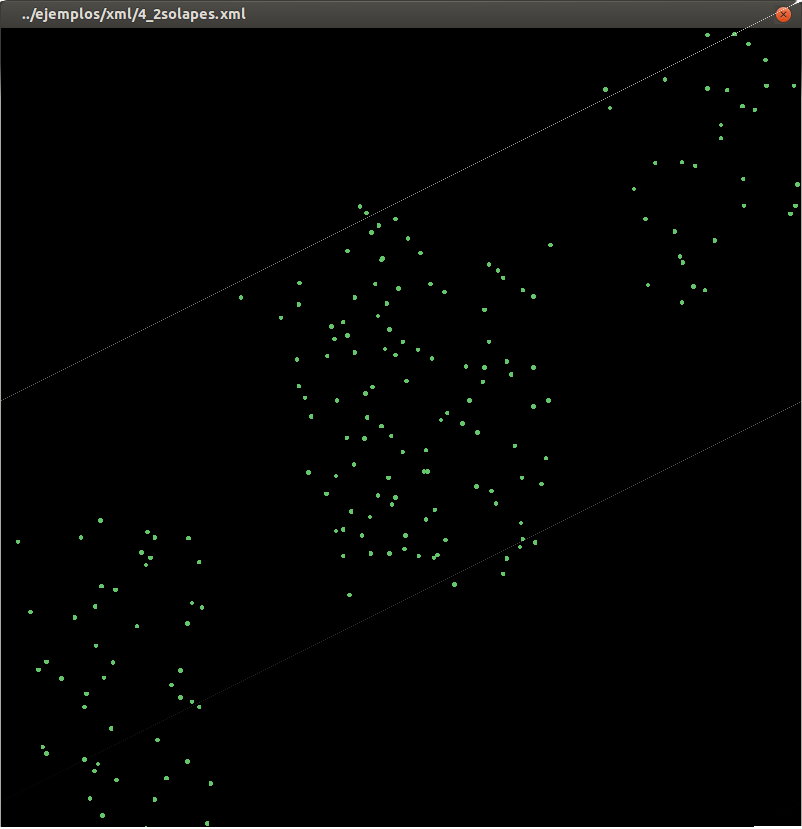
\includegraphics[width=0.5\linewidth]{4_2solapes-in}
\label{fig:4_2solapes-in}}
\subfloat[Salida del \CSUO{}]{
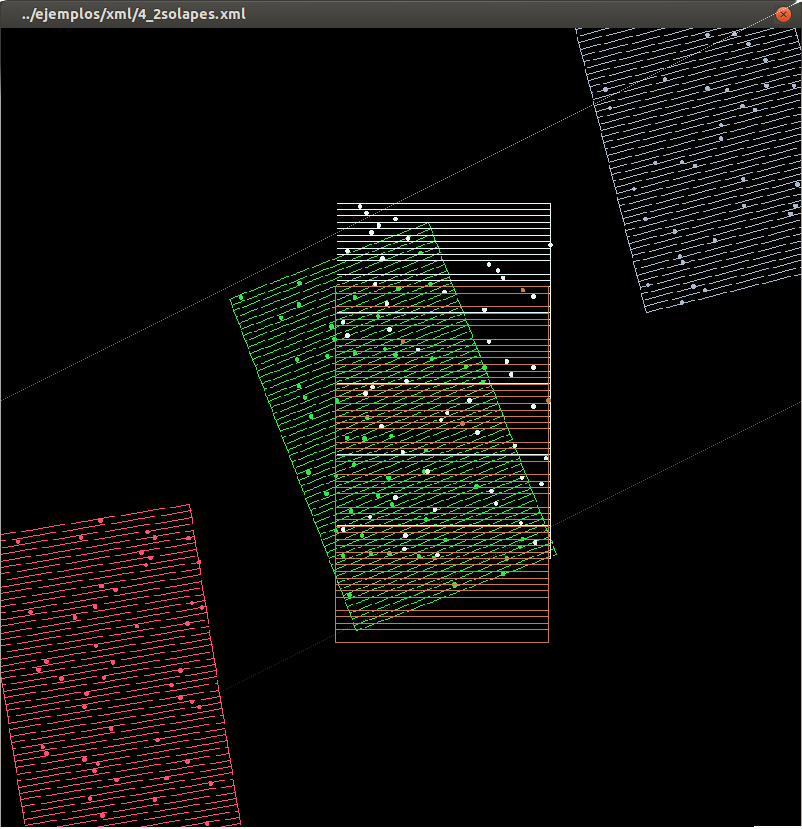
\includegraphics[width=0.5\linewidth]{4_2solapes-out}
\label{fig:4_2solapes-out}}
\caption{Ejemplo \texttt{4\_2solapes.xml}. Ejemplo de ``colisión'' de dos apuntados}
\end{figure}
%%%%%%%%%%%%%%%%%%%%%%%%%%%%%%%%%%%%%%%%%%%%%%%%%%%%%%%%%%%%%%

\begin{table*}[!ht]
\centering
\begin{tabular}{||l||c|c||}
\hline
\hline
RESULTADOS & Apuntados & Tiempo \\
\hline
\hline
Sin opciones & 5 & 4.26'' \\
\hline
Sin bordes & 5 & 3.64'' \\
\hline
Beam Switching & 5 & 4.29'' \\
\hline
Sin bordes + Beam S. & 5 & 3.67'' \\
\hline
\hline
\end{tabular}
\caption{Resultados del ejemplo \texttt{4\_2solapes.xml}}
\end{table*}

Pese al alto grado de solapamiento, la aplicación sólo ha introducido un
apuntado de más, por lo que se considera que el algoritmo ofrece resultados de razonable calidad
teniendo en cuenta el tiempo de ejecución.

\subsection {Ejemplo: \texttt{denso.xml}}
Este ejemplo no ha sido generado con la herramienta \texttt{mapEditor} sino que se
ha creado mediante una distribución aleatoria de los objetos, razón por la cual no podemos conocer a priori el
resultado óptimo. 
El ejemplo nos sirve para estudiar cómo se comporta la aplicación 
ante grandes nubes de objetos con una distribución espacial homogéneas. 
El ejemplo consta de 999 puntos.

%%%%%%%%%%%%%%%%%%%% Fig. %%%%%%%%%%%%%%%%%%%%%%%%%%%%%%%%%%%
\begin{figure}[!htb]
\centering
\subfloat[Entrada]{
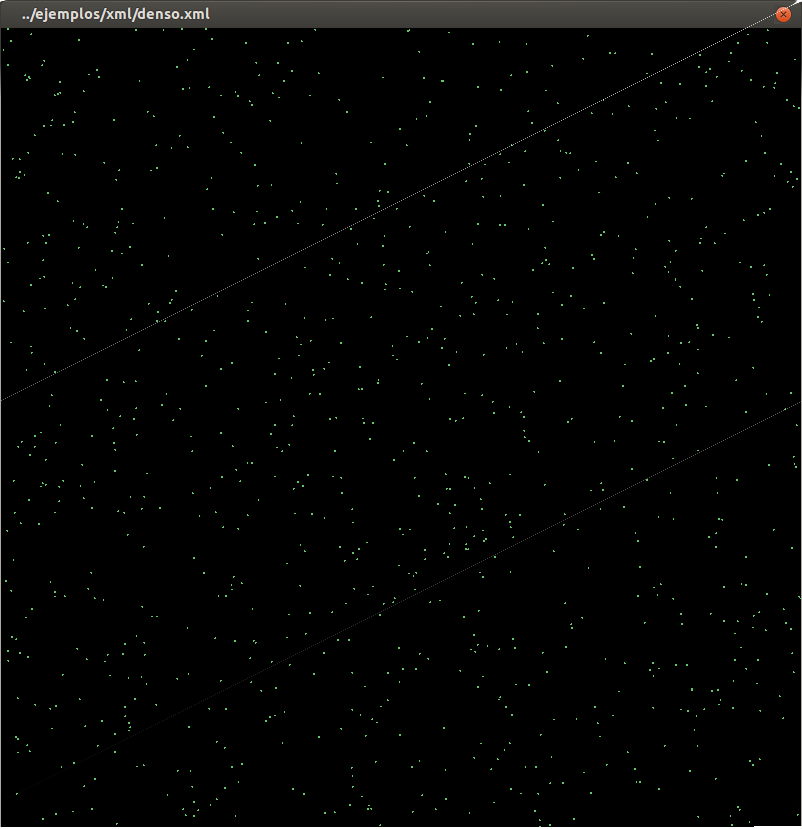
\includegraphics[width=0.5\linewidth]{denso-in}
\label{fig:denso-in}}
\subfloat[Salida del \CSUO{}]{
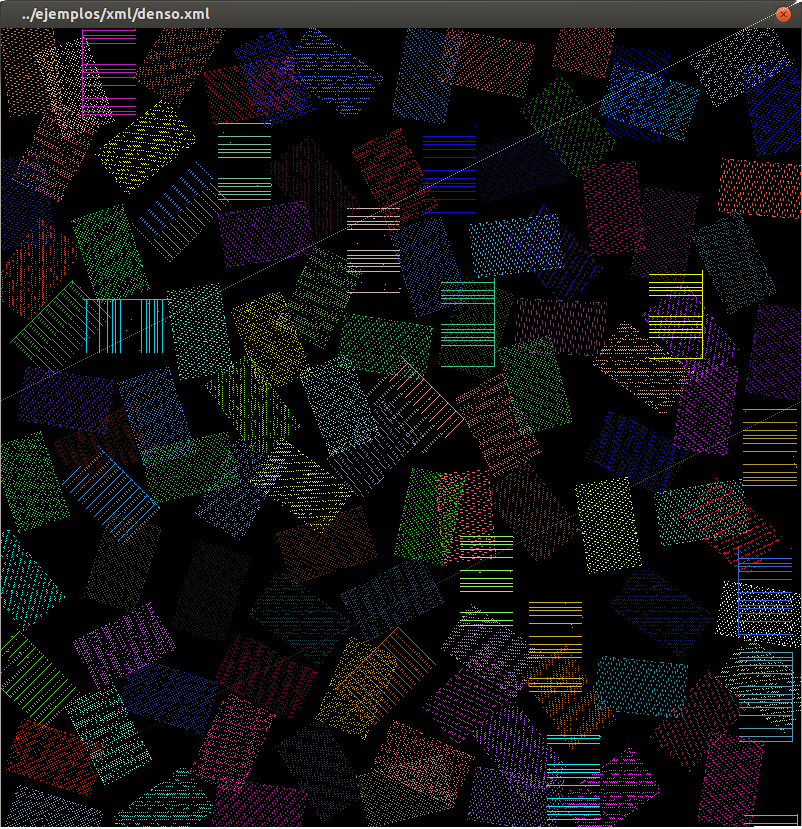
\includegraphics[width=0.5\linewidth]{denso-out}
\label{fig:denso-out}}
\caption{Ejemplo \texttt{denso.xml}. Gran número de objetos distribuidos homogéneamente}
\end{figure}
%%%%%%%%%%%%%%%%%%%%%%%%%%%%%%%%%%%%%%%%%%%%%%%%%%%%%%%%%%%%%%

\begin{table*}[!ht]
\centering
\begin{tabular}{||l||c|c||}
\hline
\hline
RESULTADOS & Apuntados & Tiempo \\
\hline
\hline
Sin opciones & 110 & 26.93'' \\
\hline
Sin bordes & 118 & 20.02'' \\
\hline
Beam Switching & 150 & 42.87'' \\
\hline
Sin bordes + Beam S. & 175 & 1' 1.78'' \\
\hline
\hline
\end{tabular}
\caption{Resultados del ejemplo \texttt{denso.xml}}
\label{tabla:denso}
\end{table*}

\subsection {Ejemplo: \texttt{denso2000.xml}}
Se trata del mismo ejemplo anterior, incrementando el número de objetos hasta 2000. 
Esta entrada se generó con el fin de evaluar el tiempo tarda el \CSUO{} en generar soluciones para ejemplos
relativamente grandes.

%%%%%%%%%%%%%%%%%%%% Fig. %%%%%%%%%%%%%%%%%%%%%%%%%%%%%%%%%%%
\begin{figure}[!htb]
\centering
\subfloat[Entrada]{
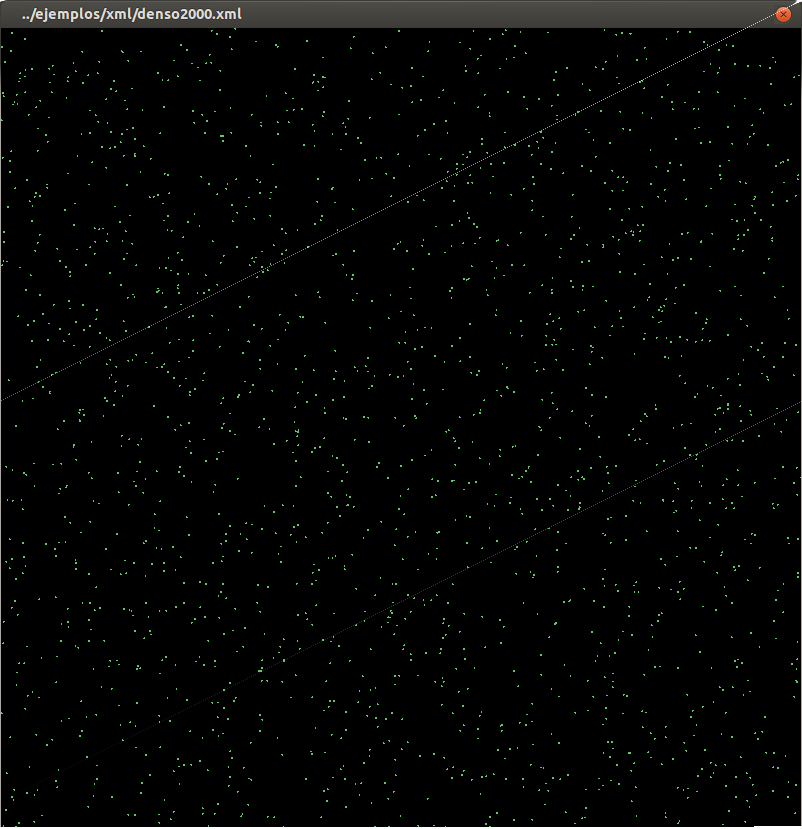
\includegraphics[width=0.5\linewidth]{denso2000-in}
\label{fig:denso2000-in}}
\subfloat[Salida del \CSUO{}]{
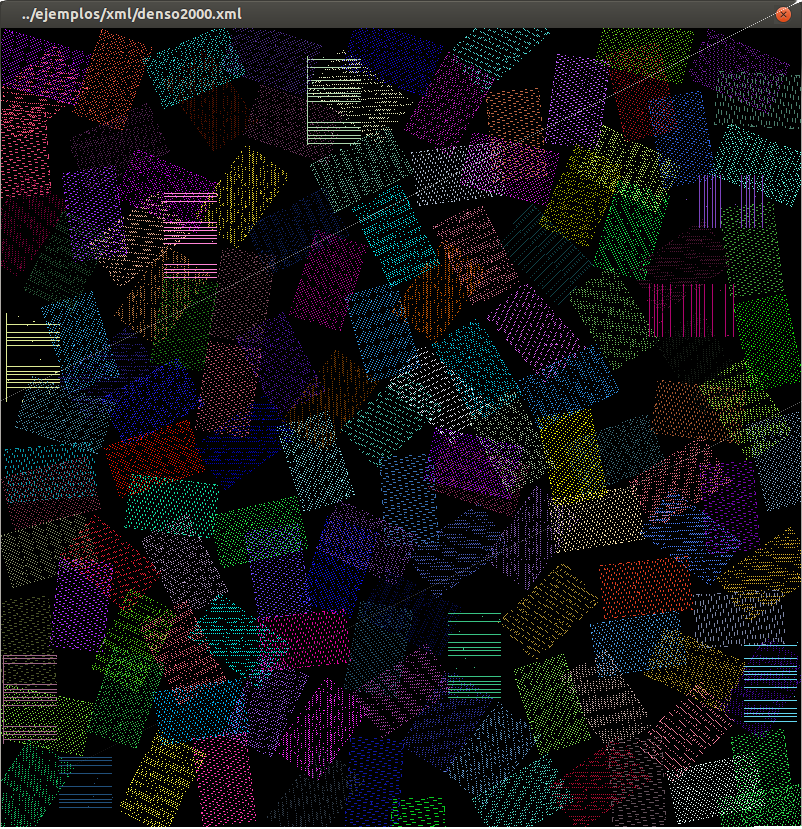
\includegraphics[width=0.5\linewidth]{denso2000-out}
\label{fig:denso2000-out}}
\caption{Ejemplo \texttt{denso2000.xml}. 2000 objetos generados aleatoriamente y distribuidos de forma homogénea}
\end{figure}
%%%%%%%%%%%%%%%%%%%%%%%%%%%%%%%%%%%%%%%%%%%%%%%%%%%%%%%%%%%%%%

\begin{table*}[!ht]
\centering
\begin{tabular}{||l||c|c||}
\hline
\hline
RESULTADOS & Apuntados & Tiempo \\
\hline
\hline
Sin opciones & 135 & 1' 42.69'' \\
\hline
Sin bordes & 152 & 2' 17.52'' \\
\hline
Beam Switching & 217 & 3' 44.53'' \\
\hline
Sin bordes + Beam S. & 296 & 3' 20.97'' \\
\hline
\hline
\end{tabular}
\caption{Resultados del ejemplo \texttt{denso2000.xml}}
\end{table*}

Si se comparan los resultados del ejemplo anterior (Tabla \ref{tabla:denso}) con
los de este caso, se comprueba que los tiempos no aumentan linealmente conforme
aumenta el tamaño del problema: se han duplicado los objetos pero los tiempos no
presentan esta proporcionalidad. 
% XXX <-- Ojo a esa afirmación: los tiempos a lo mejor no se doblan de forma exacta, pero no estoy seguro de lo que dices.
% Comentame algo al respecto.
Este efecto se debe a que el tiempo final no depende tanto del número de
puntos sino de cómo estos están distribuidos espacialmente. 
A mayor número de colisiones, mayor número de comprobaciones tendrá que hacer la aplicación.

\subsection {Ejemplo: \texttt{disperso.xml}}
Este ejemplo consta de 200 objetos repartidos aleatoriamente, de forma que no se
formen nubes de gran densidad, obteniendo así un caso en el que los objetos 
tienen una cierta distancia entre ellos. Es este caso el número de apuntados
debería ser cercano al número de objetos, puesto que con esta disposición es
poco probable encontrar grupos cercanos agrupables en una única CSU.

%%%%%%%%%%%%%%%%%%%% Fig. %%%%%%%%%%%%%%%%%%%%%%%%%%%%%%%%%%%
\begin{figure}[!htb]
\centering
\subfloat[Entrada]{
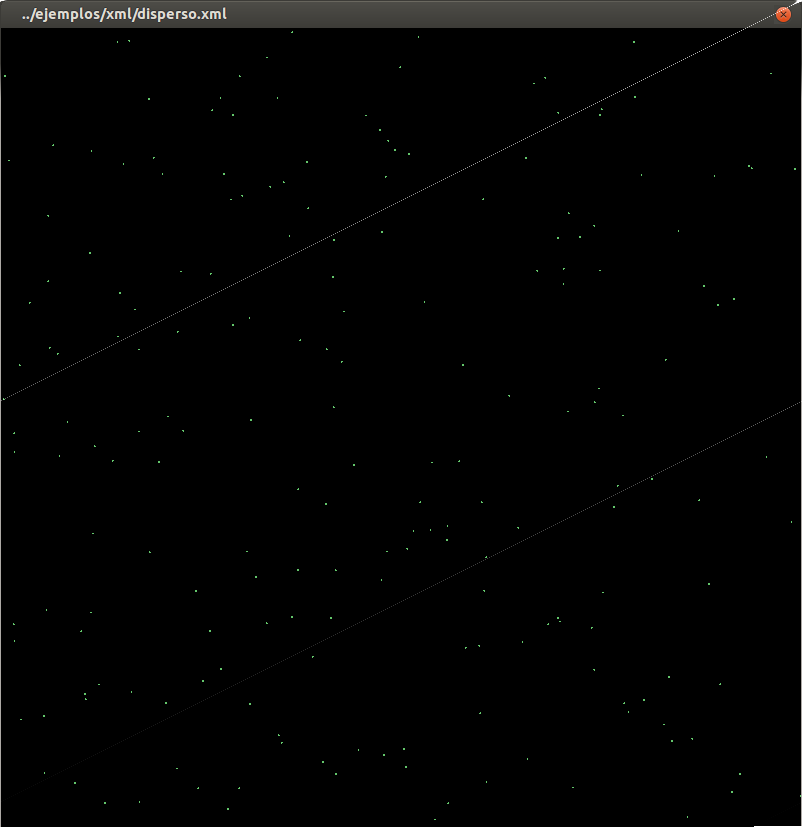
\includegraphics[width=0.5\linewidth]{disperso-in}
\label{fig:disperso-in}}
\subfloat[Salida del \CSUO{}]{
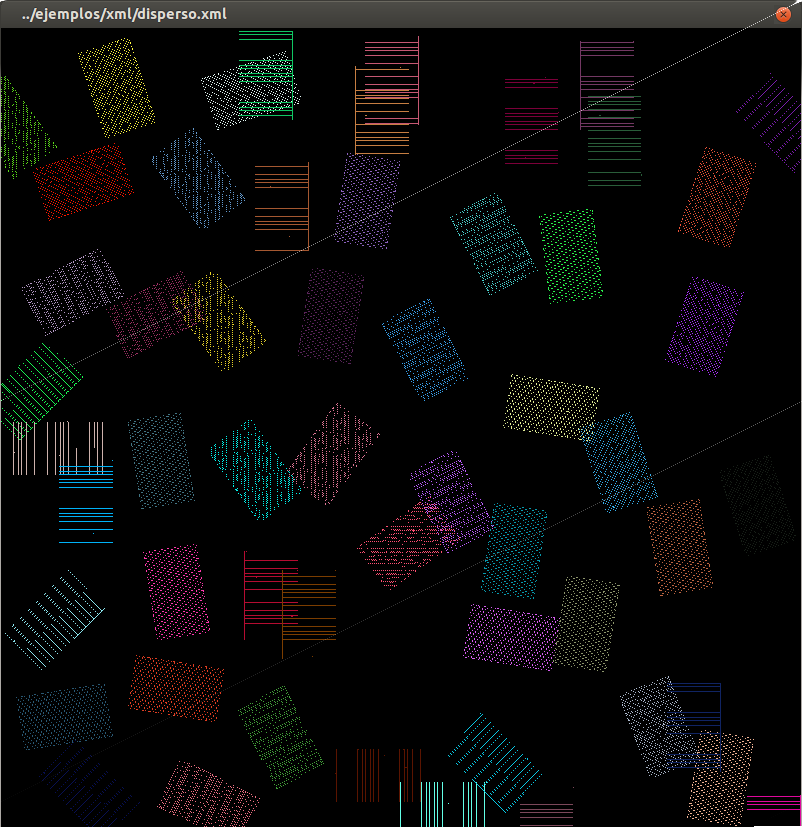
\includegraphics[width=0.5\linewidth]{disperso-out}
\label{fig:disperso-out}}
\caption{Ejemplo \texttt{disperso.xml}. 200 objetos distribuidos en un campo de un grado cuadrado}
\end{figure}
%%%%%%%%%%%%%%%%%%%%%%%%%%%%%%%%%%%%%%%%%%%%%%%%%%%%%%%%%%%%%%

\begin{table*}[!ht]
\centering
\begin{tabular}{||l||c|c||}
\hline
\hline
RESULTADOS & Apuntados & Tiempo \\
\hline
\hline
Sin opciones & 55 & 2.20'' \\
\hline
Sin bordes & 55& 2.16'' \\
\hline
Beam Switching & 61 & 2.66'' \\
\hline
Sin bordes + Beam S. & 67& 2.85'' \\
\hline
\hline
\end{tabular}
\caption{Resultados del ejemplo \texttt{disperso.xml}}
\end{table*}

El número de apuntados obtenido presenta una media de unos 4 objetos por
apuntado, significativamente inferior a su capacidad de 55 objetos, como cabe esperar 
de la baja densidad del ejemplo.

\subsection {Ejemplo: \texttt{clusters.xml}}
Para este ejemplo se han generado tres nubes de objetos separadas entre
si, cuyos objetos están dispuestos aleatoriamente, impidiendo conocer a priori
el resultado óptimo. El número total de objetos es de 146.
El objetivo de esta prueba era comprobar que la función
que reduce las colisiones no trataba apuntados o elementos que estuvieran
separados.
%%%%%%%%%%%%%%%%%%%% Fig. %%%%%%%%%%%%%%%%%%%%%%%%%%%%%%%%%%%
\begin{figure}[!htb]
\centering
\subfloat[Entrada]{
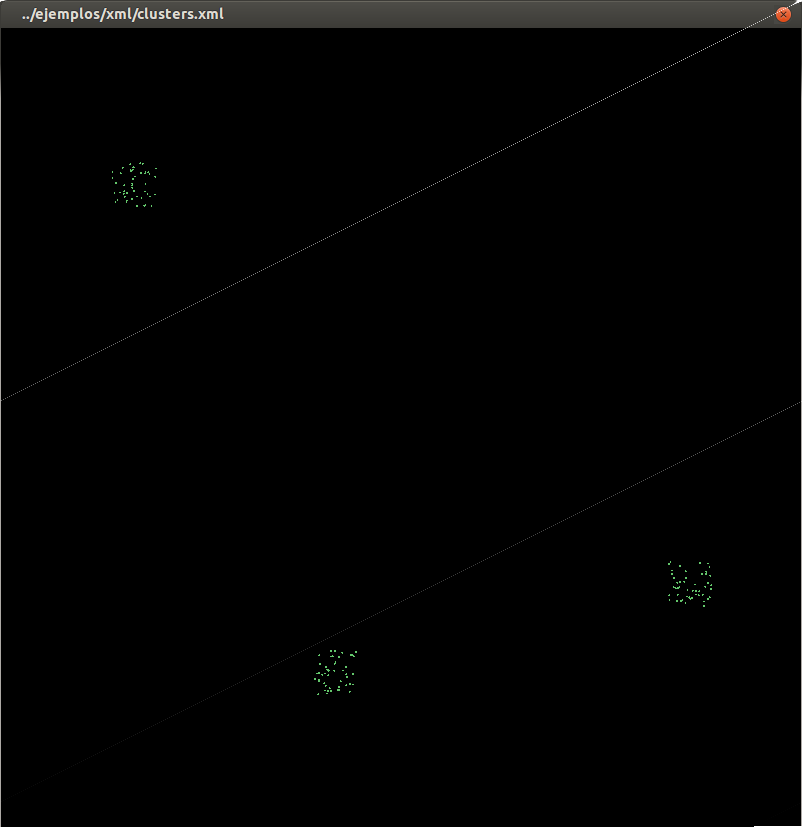
\includegraphics[width=0.5\linewidth]{clusters-in} 
\label{fig:clusters-in}}
\subfloat[Salida del \CSUO{}]{
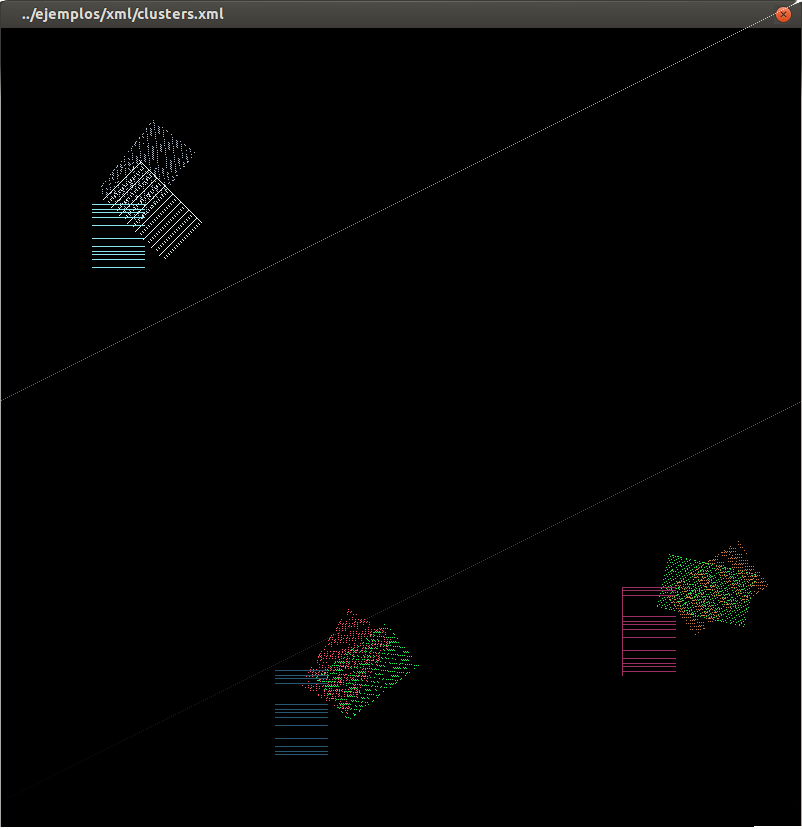
\includegraphics[width=0.5\linewidth]{clusters-out}
\label{fig:clusters-out}}
\caption{Ejemplo \texttt{clusters.xml}. Pequeño grupo de objetos agrupados en tres clústers independientes}
\end{figure}
%%%%%%%%%%%%%%%%%%%%%%%%%%%%%%%%%%%%%%%%%%%%%%%%%%%%%%%%%%%%%%

\begin{table*}[!ht]
\centering
\begin{tabular}{||l||c|c||}
\hline
\hline
RESULTADOS & Apuntados & Tiempo \\
\hline
\hline
Sin opciones & 9 & 2.79'' \\
\hline
Sin bordes &9 & 2.69'' \\
\hline
Beam Switching & 12 & 5.18'' \\
\hline
Sin bordes + Beam S. & 15& 5.43'' \\
\hline
\hline
\end{tabular}
\caption{Resultados del ejemplo \texttt{clusters.xml}}
\end{table*}

\section{Ejemplos reales}
En esta sección se presentan ejemplos que no han sido generados de manera
sintética como los anteriores, sino que han sido aportados por el responsable del
proyecto EMIR para comprobar el funcionamiento de la aplicación ante distribuciones de
objetos reales (o al menos más realistas).

\subsection {Ejemplo: \texttt{real1.xml}}
Este ejemplo ha sido clave para comprobar la calidad de los resultados
obtenidos, puesto que se conoce a priori el número óptimo de apuntados
necesarios para resolverlo, siendo este valor de 65 apuntados. El ejemplo
consta de un conjunto de aproximadamente 2000 objetos dispersos en un campo de un
grado cuadrado, esto es, 3600$\times$3600 arcosegundos.

%%%%%%%%%%%%%%%%%%%% Fig. %%%%%%%%%%%%%%%%%%%%%%%%%%%%%%%%%%%
\begin{figure}[!htb]
\centering
\subfloat[Entrada]{
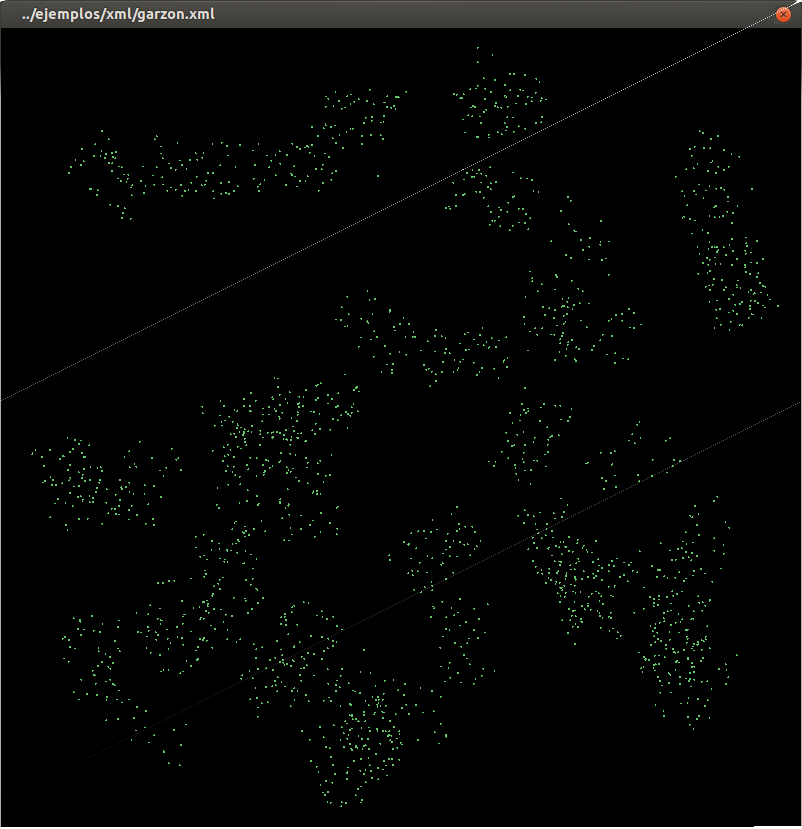
\includegraphics[width=0.5\linewidth]{real1-in} 
\label{fig:real1-in}}
\subfloat[Salida del \CSUO{}]{
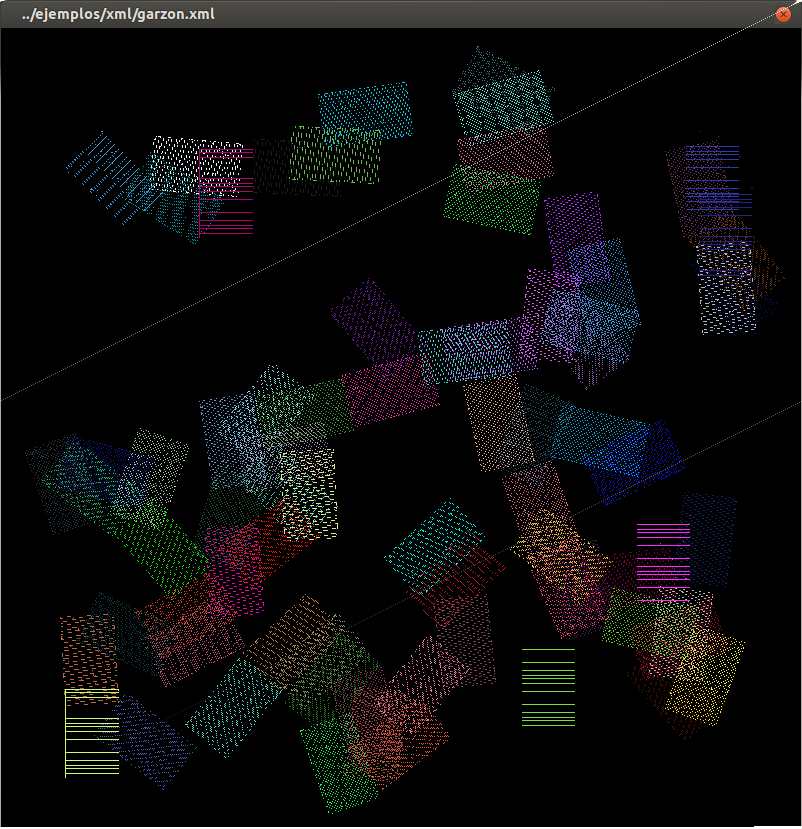
\includegraphics[width=0.5\linewidth]{real1-out}
\label{fig:real1-out}}
\caption{Ejemplo \texttt{real1.xml}. Caso real de 2000 objetos que siguen una distribución uniforme}
\end{figure}
%%%%%%%%%%%%%%%%%%%%%%%%%%%%%%%%%%%%%%%%%%%%%%%%%%%%%%%%%%%%%%

\begin{table*}[!ht]
\centering
\begin{tabular}{||l||c|c||}
\hline
\hline
RESULTADOS & Apuntados & Tiempo \\
\hline
\hline
Sin opciones & 75 & 2' 53.69'' \\
\hline
Sin bordes &91 & 2' 3.21'' \\
\hline
Beam Switching & 142 & 4' 1.28'' \\
\hline
Sin bordes + Beam S. & 181& 5' 33.68'' \\
\hline
\hline
\end{tabular}
\caption{Resultados del ejemplo \texttt{real1.xml}}
\end{table*}

El resultado obtenido se acerca al óptimo, dando 10 apuntados más de
los deseados. Puede verse como una extensión del problema \texttt{4\_2solapes}
analizado anteriormente. Al existir mucho solape entre apuntados, el algoritmo
tarda al intentar reducirlos, aunque no siempre toma la mejor elección
posible de objetos, situando en un apuntado un elemento que iría mejor en otro.
No obstante el resultado es razonablemente bueno, confirmando nuestra hipótesis sobre
el buen funcionamiento del algoritmo.

\subsection {Ejemplo: \texttt{real2.xml}}
El ejemplo que sigue a continuación tiene una cantidad de objetos mucho menor a
la que podríamos esperar de un caso real, puesto que consta solamente de 297
objetos. Se desconoce su resultado óptimo.

%%%%%%%%%%%%%%%%%%%% Fig. %%%%%%%%%%%%%%%%%%%%%%%%%%%%%%%%%%%
\begin{figure}[!htb]
\centering
\subfloat[Entrada]{
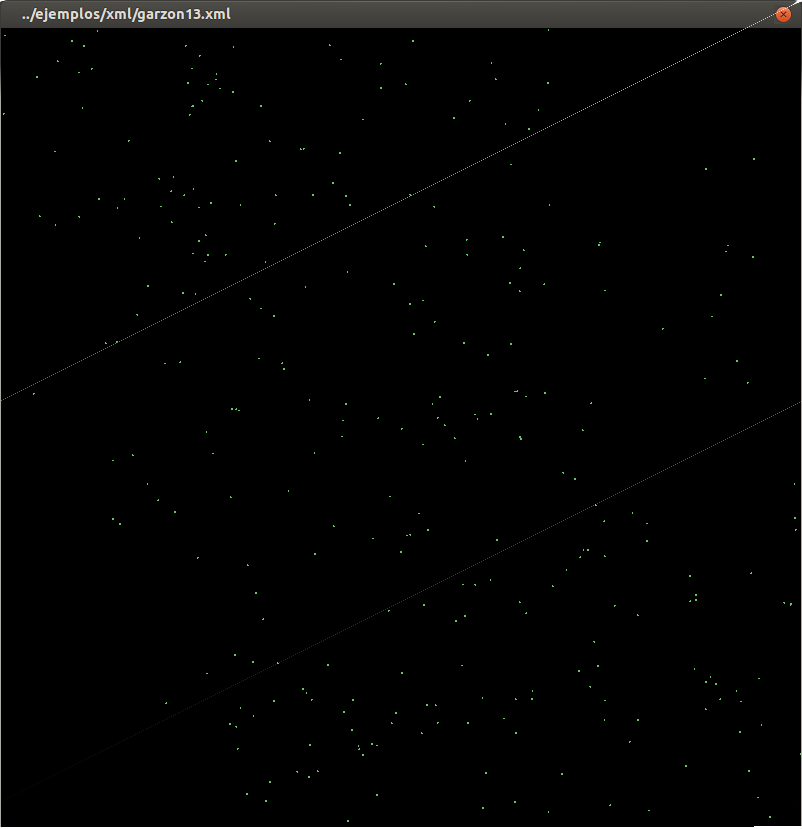
\includegraphics[width=0.5\linewidth]{real2-in} 
\label{fig:real2-in}}
\subfloat[Salida del \CSUO{}]{
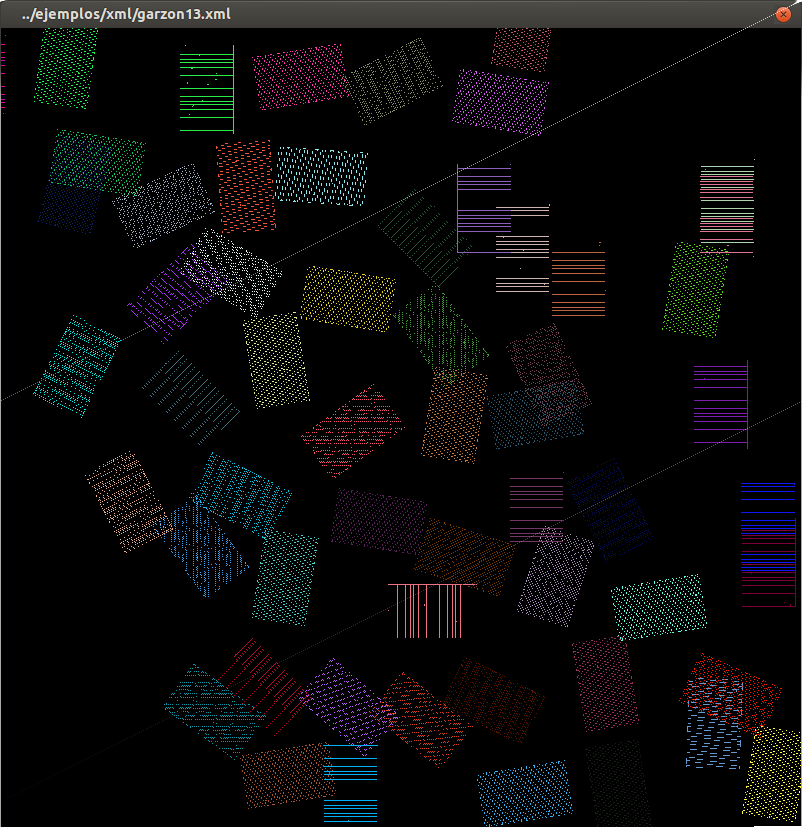
\includegraphics[width=0.5\linewidth]{real2-out}
\label{fig:real2-out}}
\caption{Ejemplo \texttt{real2.xml}. Aproximadamente 300 objetos reales}
\end{figure}
%%%%%%%%%%%%%%%%%%%%%%%%%%%%%%%%%%%%%%%%%%%%%%%%%%%%%%%%%%%%%%

\begin{table*}[!ht]
\centering
\begin{tabular}{||l||c|c||}
\hline
\hline
RESULTADOS & Apuntados & Tiempo \\
\hline
\hline
Sin opciones & 57 & 3.85'' \\
\hline
Sin bordes & 56 & 3.91'' \\
\hline
Beam Switching & 70 & 6.24'' \\
\hline
Sin bordes + Beam S. & 79& 7.08'' \\
\hline
\hline
\end{tabular}
\caption{Resultados del ejemplo \texttt{real2.xml}}
\end{table*}

En el segundo caso, en el cual se ejecuta la opción de quitar un mínimo espacio
a los bordes, obtenemos un mejor resultado. Esto se debe, como podemos intuir,
a que al obligar que los objetos se sitúen en un espacio más reducido, es
posible que la forma en la que se coloquen evite que un elemento que
antiguamente nos producía un mal intercambio de puntos entre a formar parte del
apuntado.

\subsection {Ejemplo: \texttt{cluster1.xml}}
El siguiente ejemplo es un caso real con 1398 objetos situados formando un
círculo alrededor del centro de un espacio de 4187 arcosegundos de ancho por
4183 arcosegundos de alto.

%%%%%%%%%%%%%%%%%%%% Fig. %%%%%%%%%%%%%%%%%%%%%%%%%%%%%%%%%%%
\begin{figure}[!htb]
\centering
\subfloat[Entrada]{
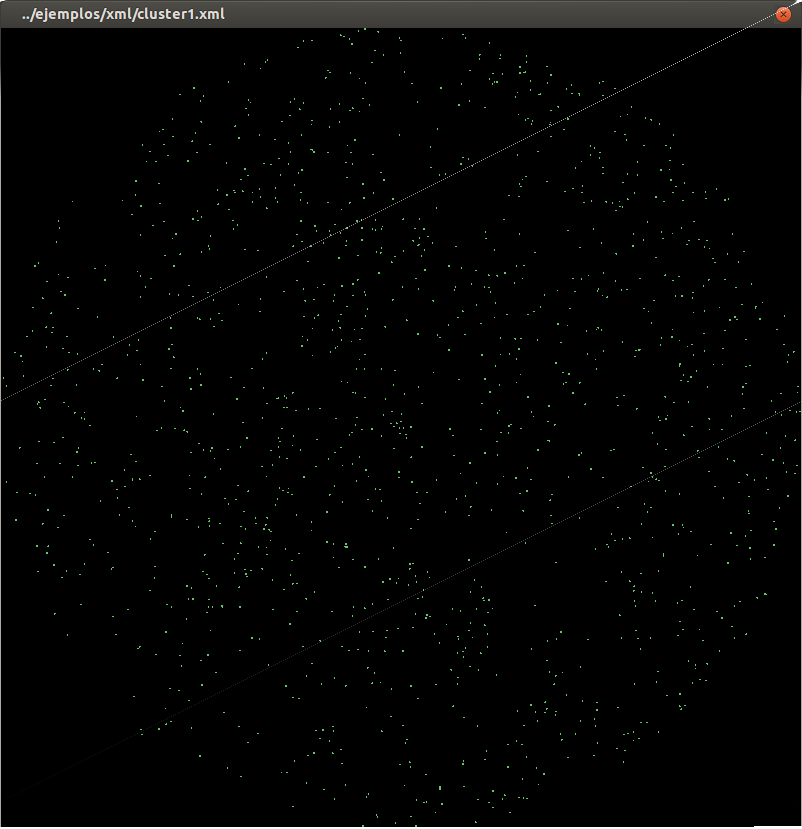
\includegraphics[width=0.5\linewidth]{cluster1-in} 
\label{fig:cluster1-in}}
\subfloat[Salida del \CSUO{}]{
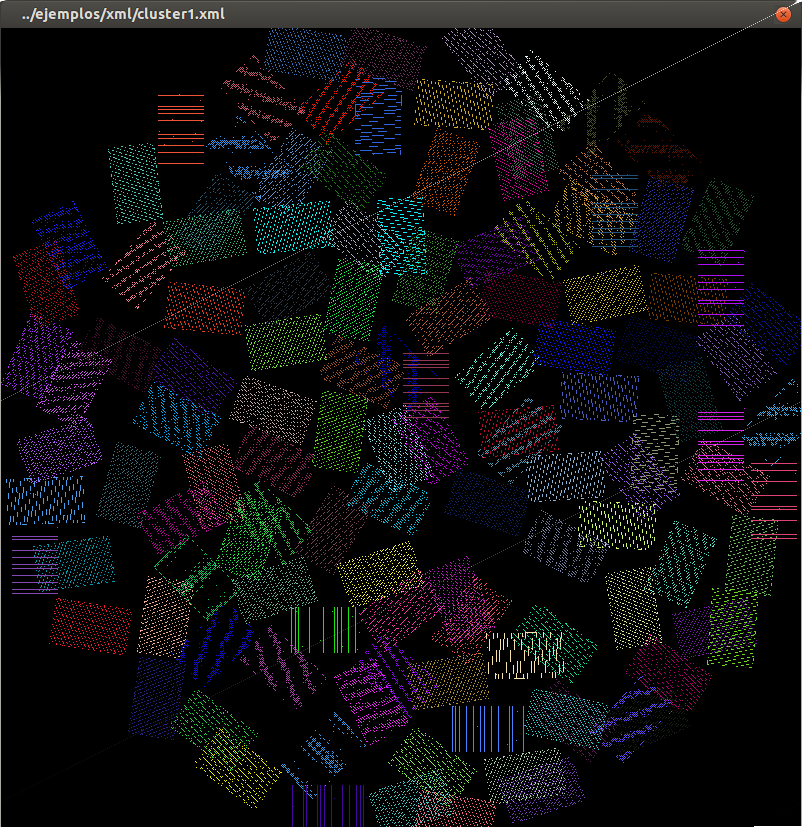
\includegraphics[width=0.5\linewidth]{cluster1-out}
\label{fig:cluster1-out}}
\caption{Ejemplo \texttt{cluster1.xml}. Caso real cuyos objetos muestran una distribución concéntrica.}
\end{figure}
%%%%%%%%%%%%%%%%%%%%%%%%%%%%%%%%%%%%%%%%%%%%%%%%%%%%%%%%%%%%%%

\begin{table*}[!ht]
\centering
\begin{tabular}{||l||c|c||}
\hline
\hline
RESULTADOS & Apuntados & Tiempo \\
\hline
\hline
Sin opciones & 123 & 45.04'' \\
\hline
Sin bordes &138 & 45.05'' \\
\hline
Beam Switching & 180 & 1' 29.35'' \\
\hline
Sin bordes + Beam S. & 218 & 1' 59.17'' \\
\hline
\hline
\end{tabular}
\caption{Resultados del ejemplo \texttt{cluster1.xml}}
\end{table*}

\subsection {Ejemplo: \texttt{cluster2.xml}}
Este caso es similar al anterior, consta de 1842 elementos, aproximadamente 400
objetos más que antes, por lo que podríamos suponer un aumento considerable en
los tiempos de ejecución. Sin embargo, como ya hemos comentado anteriormente, el
tiempo depende más de la disposición de los elementos que de su número, aunque, 
debido a la semejanza entre los ejemplos, asumimos que son condiciones iguales
con un mayor número de puntos y esperamos tiempos mayores.

%%%%%%%%%%%%%%%%%%%% Fig. %%%%%%%%%%%%%%%%%%%%%%%%%%%%%%%%%%%
\begin{figure}[!htb]
\centering
\subfloat[Entrada]{
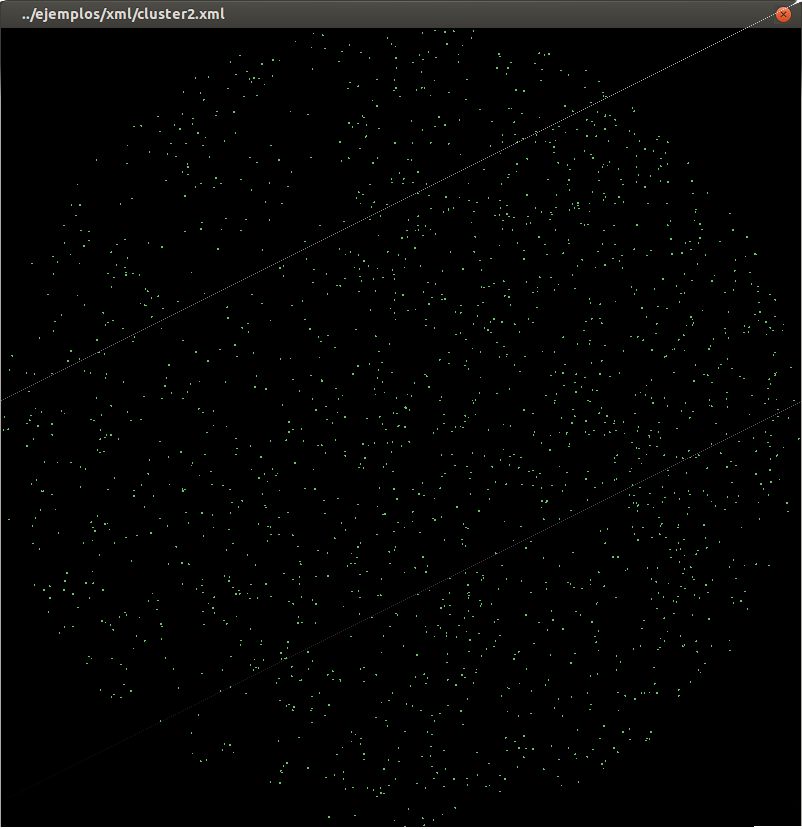
\includegraphics[width=0.5\linewidth]{cluster2-in} 
\label{fig:cluster2-in}}
\subfloat[Salida del \CSUO{}]{
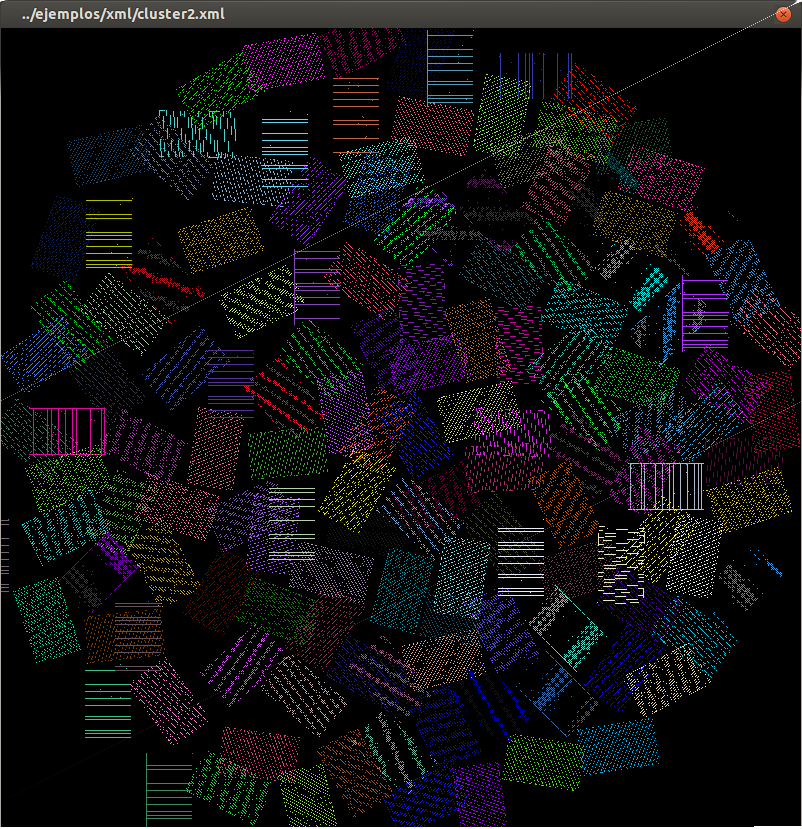
\includegraphics[width=0.5\linewidth]{cluster2-out}
\label{fig:cluster2-out}}
\caption{Ejemplo \texttt{cluster2.xml}. Segundo ejemplo cuyos objetos muestran una distribución concéntrica.}
\end{figure}
%%%%%%%%%%%%%%%%%%%%%%%%%%%%%%%%%%%%%%%%%%%%%%%%%%%%%%%%%%%%%%

\begin{table*}[!ht]
\centering
\begin{tabular}{||l||c|c||}
\hline
\hline
RESULTADOS & Apuntados & Tiempo \\
\hline
\hline
Sin opciones & 138 & 1' 57.42'' \\
\hline
Sin bordes & 152& 2' 1.68'' \\
\hline
Beam Switching & 213 & 2' 19.05'' \\
\hline
Sin bordes + Beam S. & 263 & 4' 19.05'' \\
\hline
\hline
\end{tabular}
\caption{Resultados del ejemplo \texttt{cluster2.xml}}
\end{table*}

Como se observa en los resultados obtenidos, a pesar de que el número de
apuntados necesarios para recoger todos los objetos no es mucho mayor (una
diferencia de 15 apuntados), sí lo es el tiempo que tarda, pasando de
aproximadamente dos minutos a algo más de cuatro minutos y medio. No obstante,
si nos fijamos en el tercer caso, en el que se usa la técnica del beam
switching, vemos que con una diferencia de 33 apuntados, apenas aumenta 1 minuto
el tiempo.

\subsection {Ejemplo: \texttt{cluster3.xml}}
Este ejemplo es igual que los dos anteriores, es decir, tiene una disposición
circular y consta de 1074 objetos. Igual que en el anterior esperábamos tiempos
mayores debido a que era el ejemplo de mayor tamaño, en este esperamos mejores
tiempos al ser el que presenta menor número de elementos.

%%%%%%%%%%%%%%%%%%%% Fig. %%%%%%%%%%%%%%%%%%%%%%%%%%%%%%%%%%%
\begin{figure}[!htb]
\centering
\subfloat[Entrada]{
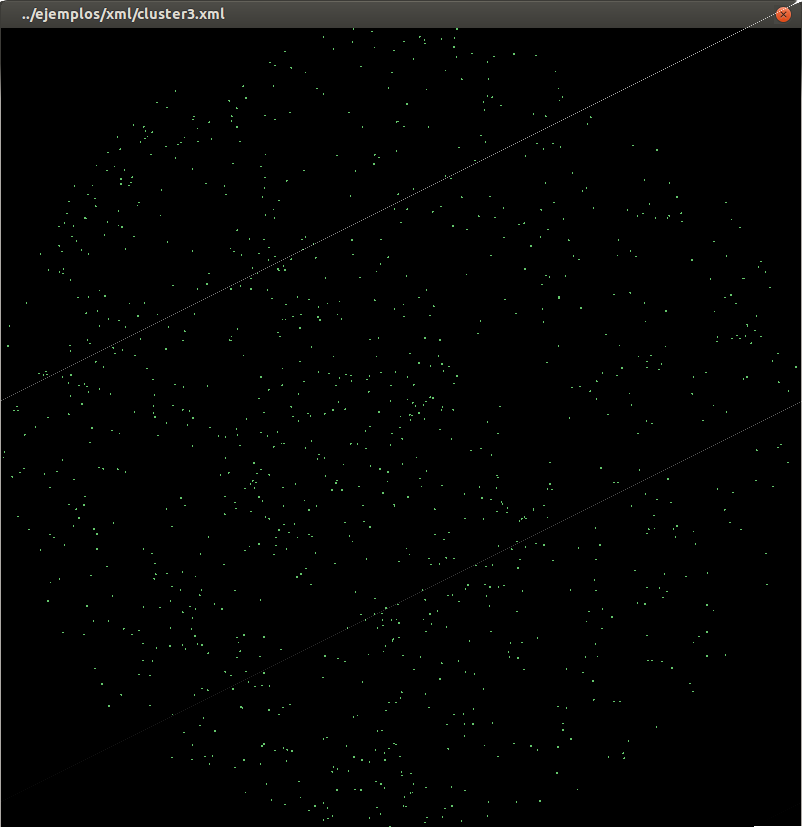
\includegraphics[width=0.5\linewidth]{cluster3-in} 
\label{fig:cluster3-in}}
\subfloat[Salida del \CSUO{}]{
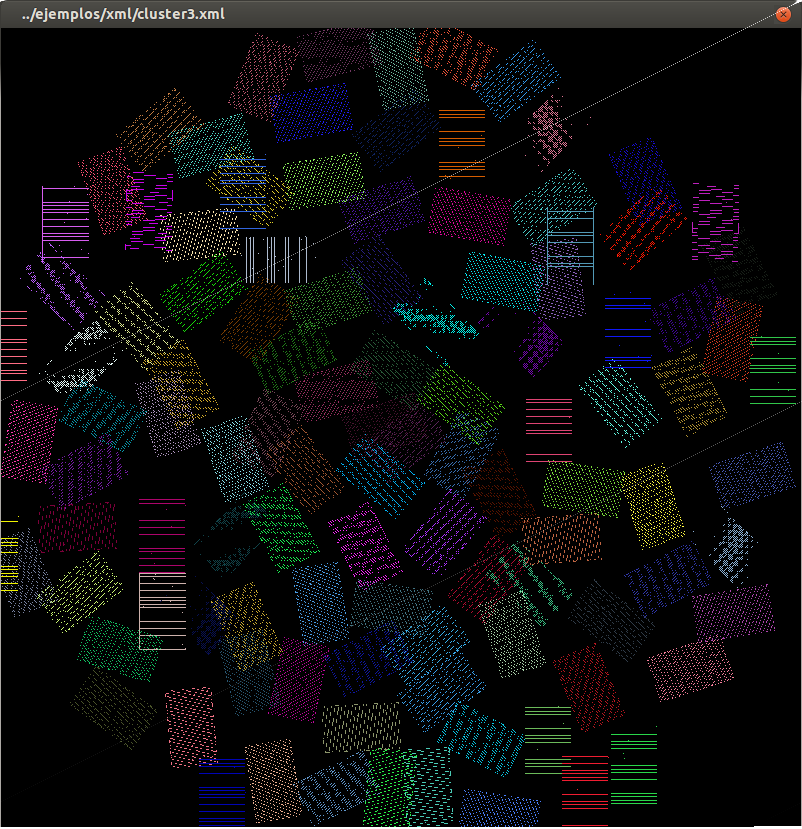
\includegraphics[width=0.5\linewidth]{cluster3-out}
\label{fig:cluster3-out}}
\caption{Ejemplo \texttt{cluster3.xml}. Tercer caso real cuyos objetos muestran una distribución concéntrica.}
\end{figure}
%%%%%%%%%%%%%%%%%%%%%%%%%%%%%%%%%%%%%%%%%%%%%%%%%%%%%%%%%%%%%%

\begin{table*}[!ht]
\centering
\begin{tabular}{||l||c|c||}
\hline
\hline
RESULTADOS & Apuntados & Tiempo \\
\hline
\hline
Sin opciones & 109 & 31.09'' \\
\hline
Sin bordes & 117 & 38.57'' \\
\hline
Beam Switching & 153 & 1' 4.49'' \\
\hline
Sin bordes + Beam S. & 180 & 1' 16.68'' \\
\hline
\hline
\end{tabular}
\caption{Resultados del ejemplo \texttt{cluster3.xml}}
\end{table*}

Los resultados obtenidos son similares a los del primer ejemplo, y no distan
tanto entre sí como los dos primeros a pesar de tener más o menos la misma
diferencia de objetos.

%
% ---------------------------------------------------
%
% Proyecto Final de Carrera: EMIR
% Autor: Pedro Hernández Martín <alu3679@etsii.ull.es>
% Capítulo: Detalles del problema
% Fichero: Cap_conclusiones.tex
%
% ----------------------------------------------------
%

\chapter{Conclusiones y Trabajos Futuros} \label{chap:conclusions}
En este PFC, se ha abordado la resolución del problema de minimización del número de apuntados
del telescopio GTC necesarios para observar mediante el instumento EMIR un conjunto de objetos
de interés astronómico.
Se trata de un problema real que tienen los investigadores del proyecto EMIR y ello ha supuesto para
el autor un acicate en nuestro esfuerzo para acreditar que somos capaces de resolver eficientemente
problemas de ingeniería.

El resultado más tangible del PFC es la aplicación \CSUO{}. 
Se trata de una pequeña aplicación escrita en C++ siguiendo el paradigma orientado a objetos de unas
3300 líneas de código.
No obstante quisiéramos destacar desde el punto de vista académico que el PFC, como no puede ser de otro modo, 
ha representado un escenario real de trabajo en el que el autor ha
podido desplegar de forma práctica técnicas, metodologías, herramientas y conceptos estudiados en los años de discencia en la ETSI Informática.

Las mayores dificultades halladas en el desarrollo del proyecto han sido:
\begin{itemize}
\item El estudio y selección de algoritmos que resuelvan el problema planteado.
\item La comprensión precisa de las características intrínsecas al problema.
\item La adaptación del lenguaje de la astronomía al campo que nos es propio de la computación.
\item La mejora de la calidad de las soluciones obtenidas por la aplicación.
\item La reducción de los tiempos de ejecución del algoritmo que finalmente se ha implementado.
\end{itemize}
Queremos destacar la importancia del trabajo de depuración y optimización del código que
compone el \CSUO{} para obtener una versión que resuelve satisfactoriamente el problema propuesto.
Asimismo es destacable el trabajo realizado por el autor para lograr elaborar un producto listo para usar 
por parte de usuarios ajenos a la informática, poniendo a su disposición esta memoria del PFC, que constituye
al mismo tiempo la mejor documentación disponible para la propia aplicación desarrollada.
Importante ha sido en el desarrollo el trabajo con las
herramientas de versionado y gestión de repositorio, sin las cuales las tareas de
depuración y publicación de \textit{release} hubieran sido mucho más tediosas.

En este documento se han revisado los logros conseguidos en la ejecución del proyecto. 
Relacionándolos directamente con los objetivos planteados inicialmente, podemos
señalar como más significativos los siguientes logros:

\begin{itemize}
\item Se ha realizado una investigación sobre posibles métodos para resolver el problema propuesto.
\item Se ha desarrollado una aplicación plenamente operativa que resuelve el problema de optimización de
      los apuntados de forma que consideramos satisfactoria.
\item El software que se entrega como resultado ha sido desarrollado teniendo en mente que posiblemente sea
      tomado como punto de partida para desarrollos ulteriores que, utilizando esta implementación como base,
			la doten de funcionalidades adicionales, particularmente en el área de interfaz de usuario.
			Este punto de vista ha obligado al autor a un trabajo concienzudo de documentación y estructuración
			razonada del código.
\item Se aporta el presente documento que constituye la documentación técnica de la aplicación desarrollada (Capítulo \ref{chap:aplication}).
      Este documento será de gran ayuda para cualquier ingeniero que tenga que hacerse cargo posterior de este desarrollo
			tanto a efectos de mejora, depuración u optimización.
\end{itemize}

Consideramos por otra parte que el problema propuesto por el equipo investigador del proyecto EMIR no queda cerrado con la
conclusión de este PFC.
Debido a las limitaciones temporales que afectan a un PFC en Informática hay diversos aspectos del trabajo realizado que
claramente cabe mejorar.
Algunas mejoras que hubieran tenido cabida en el marco del PFC no entrañan gran dificultad. 
Si no han sido desarrolladas, ello se debe a que hasta el último momento, los esfuerzos del trabajo se han centrado exclusivamente
en la mejora de las soluciones encontradas por la aplicación.
Reseñamos a continuación en forma de posibles trabajos futuros a acometer en el marco del Proyecto EMIR algunas de estas mejoras:
\begin{itemize}
\item Un estudio más concienzudo de la calidad de las soluciones que se obtienen con el \CSUO{} respecto a las soluciones óptimas
      ha quedado fuera del trabajo realizado.
\item Hay margen de mejora en cuanto a los tiempos de respuesta del \CSUO{}. 
      Aunque se encuentran dentro de los márgenes inicialmente establecidos en la especificación de requisitos, pensamos que no es un aspecto
			difícil de mejorar.
			Un análisis preliminar mediante profiling de la aplicación nos hace ser conocedores de las funciones que habría que optimizar y
			una tecnología de paralelización utilizando OpenMP se nos ocurre como la solución a implementar inicialmente.
\item La interfaz de usuario es otro aspecto que claramente merece atención en cuanto a necesidades de desarrollo.
      A pesar de que los usuarios del \CSUO{} pertenecen al ámbito científico-tecnológico, en el que hay una mayor permisividad respecto
			a las limitaciones en cuanto a interfaz de usuario de una aplicación, pensamos que estos usuarios se beneficiarían de una
			pasarela que permitiera una selección cómoda de los objetos a observar.
			En este sentido, hemos optado por elegir XML como formato de entrada de datos a la aplicación, lo cual flexibiliza la conexión con una
			futura GUI.
\end{itemize}

% ==========================================================
% ----------              Apendices                ---------
% ----------   Estan en el directorio apendices/   ---------
\appendix
%\markboth{Ejemplos de \llc{}}{Ejemplos de \llc{}}
%
% ---------------------------------------------------
%
% Proyecto Final de Carrera: EMIR
% Autor: Pedro Hernández Martín <alu3679@etsii.ull.es>
% Capítulo: Añadidos a la memoria
% Fichero: Apendices.tex
%
% ----------------------------------------------------
%
\chapter{Códigos}
\section{\texttt{colisiones}} \label{app:colis}

\begin{lstlisting}[language=C++, numbers=none,basicstyle=\ttfamily\footnotesize,
                   caption={Código de la función que reduce las colisiones
                   aleatorias},]
set<CSU> colisiones (set<CSU> lista_ini, const int &total_puntos) {
  static int finalizar;
  finalizar = 0;
  static set<Element> puntos, p_parcial;
  static set<Element>::iterator p;
  sort(lista_ini, TAMPUN);
  static set<CSU>::iterator jt, it;
  static set<CSU> porcion, no_coli;
  set<CSU> lista_fin;
  no_coli.clear();
  while (finalizar != (lista_ini.size()+no_coli.size())) {
    lista_fin.clear();
    finalizar = lista_ini.size();
    set<Element> eliminados;
    eliminados.clear();
    it = lista_ini.begin();
    while (it != lista_ini.end()){
      static bool quitable;
      quitable = true;
      jt = lista_ini.begin();
      while (jt != lista_ini.end() && quitable){
        if (it != jt && (it->colision(*jt) || jt->colision(*it))) //Si colisiona, no lo podemos quitar
          quitable = false;
        jt++;
      }
      if (quitable) {
        lista_fin.insert(*it);
        p_parcial = it->getPoints();
        for (p = p_parcial.begin(); p != p_parcial.end(); p++) 
          eliminados.insert(*p);
        static set<CSU>::iterator borrar;
        borrar = it; //Guardamos la posicion que se va a elimimar
        it++; //pasamos a mirar la siguiente
        lista_ini.erase(borrar); //    
      }                                
      else                             
        it++;                          
    }                                  
    while (eliminados.size() != total_puntos) { //mientras queden puntos por mirar
      puntos.clear();
      p_parcial.clear();
      porcion.clear();
      it = lista_ini.begin(); //it es el principio de la lista de CSUs
		  // Cogemos los puntos del primero y los colocamos en la lista de mejora 
      p_parcial = it->getPoints(); //p_parcial son todos los puntos de la primera CSU
      for (p = p_parcial.begin(); p != p_parcial.end(); p++)
        puntos.insert(*p); //insertamos todos los puntos de la primera CSU en los totales
      porcion.insert(*it); //Ponemos esa CSU en el grupo que se va a mirar
      CSU ini = *it; //Almacenamos la primera CSU
      lista_ini.erase(it); //Borramos la CSU de la lista total
      jt = lista_ini.begin(); //jt es el principio de la lista de CSUs
      // Seleccionamos todos aquellos que colisionan con el anteriormente seleccionado
      while(!lista_ini.empty() && jt != lista_ini.end()) { //comprobamos cada uno con el primero de la lista
        if (ini.colision(*jt) || jt->colision(ini)) {
          porcion.insert(*jt); //Ponemos esa CSU en el grupo que se va a mirar
          p_parcial = jt->getPoints(); //p_parcial son los puntos de esa CSU
          for (p = p_parcial.begin(); p != p_parcial.end(); p++) 
            puntos.insert(*p); //Aniadimos los puntos al total
          static set<CSU>::iterator borrar;
          borrar = jt; //Guardamos la posicion que se va a elimimar
          jt++; //pasamos a mirar la siguiente
          lista_ini.erase(borrar); //
        }
        else {
          jt++;
        }
      }
      static bool continuar;
      continuar = true;
      // Si la colision no es necesaria teoricamente, se intenta reducir
      if (puntos.size()/NUM_BARRAS < porcion.size()) {
        static bool izq_menor;
        static CSU final;
        static set<CSU>::iterator fin;
        fin = porcion.end();
        fin--;
        final = *fin;
        izq_menor = (ini.gety() < final.gety())? true : false;
        set<CSU> nuevos = sacar_apuntados(puntos);
        sort(nuevos, TAMPUN);
        //Si se ha conseguido mejorar, volvemos a insertarlos para remirarlos
        if ((nuevos.size() < porcion.size()) || (nuevos.size() == porcion.size() && nuevos.begin()->size() > porcion.begin()->size())) {
          continuar = false;
          porcion = nuevos;
          for (it = porcion.begin(); it != porcion.end(); it++)
            lista_ini.insert(*it);
        }
      }
      // Si no se ha conseguido mejorar o la colision en necesaria, quitamos la primera CSU
      if (continuar) {
        it = porcion.begin();
        lista_fin.insert(*it);
        p_parcial = it->getPoints();
        for (p = p_parcial.begin(); p != p_parcial.end(); p++) {
          eliminados.insert(*p);
        }
        porcion.erase(it);
        for (it = porcion.begin(); it != porcion.end(); it++)
          lista_ini.insert(*it);
      }
    }
    lista_ini = lista_fin;
  }
  return lista_fin;
}

\end{lstlisting}

\section{\texttt{grasp}} \label{app:grasp}

\begin{lstlisting}[language=C++, numbers=none,basicstyle=\ttfamily\footnotesize,
                   caption={Método heurístico GRASP},]
set<CSU> grasp (set<CSU> resultado, set<Element> puntos) {
  int num_sol = 5;
  int tam_entrada = resultado.size();
  sort(resultado, TAMPUN);
  set<CSU> posibles, lista[num_sol], final;
  static set<CSU>::iterator it, jt, borrar;
  set<Element> p_finales;
  //PASO 1: generar N soluciones
  for (int i = 0; i < num_sol; i++)
    lista[i] = apuntadosRandom(puntos, i);
  //PASO 2: buscar mejor solucion
  for (int i = 0; i < num_sol; i++)
    if (lista[i].size() < resultado.size())
      resultado = lista[i];
  set<CSU> resultado_previo = resultado;
  //inicializar la solucion final
  it = resultado.begin();
  while (it != resultado.end()) {
      progreso();
    jt = it;
    jt ++;
    static bool col;
    col = false;
    while (jt != resultado.end() && !col) {
      progreso();
      if (it->colision(*jt) || jt->colision(*it))
        col = true;
      jt++;
    }
    if (!col) {
      final.insert(*it);
      static set<Element> contar;
      contar = it->getPoints();
      for (set<Element>::iterator cc = contar.begin(); cc != contar.end(); cc++)
        p_finales.insert(*cc);
      borrar = it;
      it++;
      resultado.erase(borrar);
    }
    else
      it++;
  }
  //PASO 3: Aniadir los restantes de S1 a la RCL
  for (it = resultado.begin(); it != resultado.end(); it++)
    posibles.insert(*it);
  for (int i = 0; i < num_sol; i++)
    for(it = lista[i].begin(); it != lista[i].end(); it++)
      posibles.insert(*it);
  //PASO 4: Seleccionar elementos de la RCL hasta que se cubran todos los puntos
  while (p_finales.size() != puntos.size()) {
    progreso();
    static int tam_point_max, limite;
    it = jt = posibles.begin();
    tam_point_max = it->size();
    limite = 0;
    it++;
    while (it->size() == tam_point_max) {
      it++;
      limite++;
    }
    if (limite != 0)
      limite = rand() % limite;
    for (int i = 0;  i < limite; i++)
      jt++;
    final.insert(*jt);
    static set<Element> contar;
    contar = it->getPoints();
    for (set<Element>::iterator cc = contar.begin(); cc != contar.end(); cc++)
      p_finales.insert(*cc);
    posibles.erase(jt);
  }}
  //PASO 5: Intentar mejorar el resultado obtenido.
  posibles.clear();
  posibles = final;
  posibles = colisiones(posibles, puntos.size());
  if (posibles.size() < resultado_previo.size()) {
    cout << "Mejorado con " << posibles.size() << endl;
    return posibles;
  }
  else {
    cout << "GRASP inutil" << endl;
    return resultado_previo;
  }
}

\end{lstlisting}

\section{Salida \texttt{exacto.xml}} \label{app:exacto.xml}

\begin{lstlisting}[language=XML, basicstyle=\ttfamily\footnotesize]
<Apuntado>
	<X>479.1</X>
	<Y>598.787</Y>
	<PA>0</PA>
	<Configuracion>
		<Barra>93.9</Barra>
		<Barra>115.9</Barra>
		<Barra>-21.1</Barra>
		<Barra>-70.1</Barra>
		<Barra>119.9</Barra>
		<Barra>-76.1</Barra>
		<Barra>94.9</Barra>
		<Barra>55.9</Barra>
		<Barra>-52.1</Barra>
		<Barra>-17.1</Barra>
		<Barra>65.9</Barra>
		<Barra>72.9</Barra>
		<Barra>-25.1</Barra>
		<Barra>-71.1</Barra>
		<Barra>89.9</Barra>
		<Barra>83.9</Barra>
		<Barra>98.9</Barra>
		<Barra>-23.1</Barra>
		<Barra>112.9</Barra>
		<Barra>-27.1</Barra>
		<Barra>7.9</Barra>
		<Barra>35.9</Barra>
		<Barra>-67.1</Barra>
		<Barra>29.9</Barra>
		<Barra>46.9</Barra>
		<Barra>109.9</Barra>
		<Barra>-42.1</Barra>
		<Barra>30.9</Barra>
		<Barra>-25.1</Barra>
		<Barra>-30.1</Barra>
		<Barra>-37.1</Barra>
		<Barra>-58.1</Barra>
		<Barra>-3.1</Barra>
		<Barra>6.9</Barra>
		<Barra>24.9</Barra>
		<Barra>8.9</Barra>
		<Barra>-59.1</Barra>
		<Barra>68.9</Barra>
		<Barra>75.9</Barra>
		<Barra>51.9</Barra>
		<Barra>-60.1</Barra>
		<Barra>11.9</Barra>
		<Barra>21.9</Barra>
		<Barra>-28.1</Barra>
		<Barra>102.9</Barra>
		<Barra>35.9</Barra>
		<Barra>107.9</Barra>
		<Barra>52.9</Barra>
		<Barra>-36.1</Barra>
		<Barra>-20.1</Barra>
		<Barra>112.9</Barra>
		<Barra>-9.1</Barra>
		<Barra>117.9</Barra>
		<Barra>86.9</Barra>
		<Barra>-70.1</Barra>
	</Configuracion>
</Apuntado>
\end{lstlisting}


%\include{apendices/ap_ejemplos}
%\include{apendices/ap_TrabEjemplos}
%\include{apendices/ap_correoActualizacion}
%\include{apendices/serverCfg}
%\chapter{Ficheros \textit{Makefile}}
%\lstset{language=ksh, basicstyle=\footnotesize}
%\markboth{Ficheros \textit{Makefile}}{Ficheros \textit{Makefile}}
% ==========================================================
% ---------          Bibliografia               ------------
% --------- Estan en el directorio bibliografia/------------
\pagestyle{fancy}
\markboth{Bibliography}{Bibliography}
\addcontentsline{toc}{chapter}{Bibliography}
%\chapter*{Bibliografía}
% ELEGIR un estilo que te guste de bibliografía
%\bibliographystyle{amsplain}
%\bibliographystyle{abbrv}         % 
\bibliographystyle{bmc_article}    % Este estilo mete las URLs de la bibliografía entre brackets
% 
% Diferentes ejemplos de estilos para bibliografía:
% http://amath.colorado.edu/documentation/LaTeX/reference/faq/bibstyles.html
%
\bibliography{bibliografia/bibliografia}

% ==========================================================
% ---------                Índices              ------------
% ==========================================================
\newpage 
\markboth{Índice de figuras}{Índice de figuras}
\addcontentsline{toc}{chapter}{Índice de figuras}  % Para incluirlo en el índice  
\listoffigures

\newpage 
\markboth{Índice de tablas}{Índice de tablas}
\renewcommand{\listtablename}{Índice de tablas}   %  Para que no aparezca Índice de cuadros
\addcontentsline{toc}{chapter}{Índice de tablas}  % Para incluirlo en el índice  
\listoftables

\newpage 
\markboth{Índice de listados}{Índice de listados}
\renewcommand{\lstlistlistingname}{Índice de listados} %  Para que no aparezca Listings
\addcontentsline{toc}{chapter}{Índice de listados}     % Para incluirlo en el índice     
\lstlistoflistings
\end{document}
